\documentclass[a4paper, 11pt]{article}
\pdfoutput=1 % if your are submitting a pdflatex (i.e. if you have
             % images in pdf, png or jpg format)

\usepackage{jcappub} % for details on the use of the package, please
                     % see the JCAP-author-manual

\usepackage[T1]{fontenc} % if needed

\usepackage{array}
\usepackage{enumitem}
\usepackage{graphicx}
\usepackage{epstopdf, epsfig}
\usepackage{subcaption}
\usepackage{tikz}
\usetikzlibrary{intersections}
\usepackage{pgfplots}
\usepackage{ environ}
\usepackage{framed}
\usepackage{bm}
\usepackage[us,12hr]{datetime}
\usepackage{algorithmic}
\usepackage[ruled]{algorithm2e}
\usepackage[british]{babel}

\title{Caustic skeleton of the cosmic web: non-linear constraint realizations of structural components; the 2D case}

\author[a,b]{Job Feldbrugge}
\author[c]{Rien van de Weygaert}

\affiliation[a]{Higgs Centre for Theoretical Physics, University of Edinburgh, Edinburgh, Scotland, EH8 9YL}
\affiliation[b]{Physics department, Carnegie Mellon University, Pittsburgh, United States}
\affiliation[c]{Kapteyn Astronomical Institute, University of Groningen, Groningen, The Netherlands}

\emailAdd{Job.Feldbrugge@ed.ac.uk}

\newcommand{\aap}{Astron. Astrophys.}
\newcommand{\mnras}{Mon. Not. R. Astron. Soc.}
\newcommand{\apj}{Astrophys. J.}
\newcommand{\jcap}{Journal of Cosmology and Astroparticle Physics}
\newcommand{\nat}{Nature}
\newcommand{\apjs}{Astrophysical Journal, Supplement}
\newcommand{\apjl}{Astrophysical Journal, Letters}
\newcommand{\aj}{Astronomical Journal}
\newcommand{\prd}{Physical Review D}

\newcommand{\Remark}[1]      {{\small {\textcolor{red}{  \sf{[[{#1}]]}}}}} 

\newtheorem{thr}{Theorem:}
\newtheorem{lemma}{Lemma}
\newtheorem{corollary}{Corollary}

\abstract{
\noindent 
The cosmic web consists of a complex configuration of voids, walls, filaments, and clusters, which formed under the gravitational collapse of Gaussian fluctuations. Understanding under what conditions these different structures emerge from simple initial conditions, and how different cosmological models influence their evolution, is central to the study of the large-scale structure. Here, we present a general formalism for setting up Gaussian random initial conditions satisfying non-linear constraints for specialized $N$-body simulations. These allow us to link the non-linear conditions on the eigenvalue and eigenvector fields of the deformation tensor, as specified by caustic skeleton theory, to the current-day cosmic web. By extending constraint Gaussian random field theory, and the corresponding Hoffman-Ribak algorithm, to non-linear constraints, we can probe the statistical properties of the progenitors of the walls, filaments, and clusters of the cosmic web. Applied to cosmological $N$-body simulations, the proposed techniques pave the way towards a systematic investigation of the evolution of the progenitors of the present-day walls, filaments, and clusters, and the embedded galaxies, putting flesh on the bones of the caustic skeleton. The developed non-linear constraint random field theory is valid for generic cosmological conditions. For ease of visualization, the case study presented here probes the two-dimensional caustic skeleton.

% Last compiled on: {\color{red} \currenttime\ at \today}
}

\graphicspath{
{./figures/}}

\begin{document}
%\pagecolor{yellow!30!orange}
\maketitle

%%%%%%%%%%%%%%%%%%%%%%%%%%%%%%%%%%%%%%%%%%%%%%%%%%%%%%%%%%%%%%%%
\section{Introduction}
In this study, we extend and elaborate our analytical model for the formation of the cosmic web \cite{Zeldovich:1970,Bond:1996,Weygaert:2008}, and its complex multiscale network of filaments and sheets, by the Caustic Skeleton model \cite{Feldbrugge:2018}. The formalism, expressions, and details were introduced and extensively described in \cite{Feldbrugge:2018}. It entails an exact and computationally practical set of expressions for inferring the full two- or three-dimensional skeleton of the cosmic web\footnote{The caustic conditions underlying the model that are derived in \cite{Feldbrugge:2018} are applicable for any $N$-dimensional space} emerging from any cosmological primordial field of linear density and velocity perturbations. It extends the early studies by the Soviet mathematician Arnold and collaborators \cite{Arnold:1982a,Arnold:1982b}, that studied the caustic structure predicted by the Zel'dovich formalism \cite{Zeldovich:1970}.

While the Caustic Skeleton details the structural outline of the nodes, filamentary branches, and sheetlike membranes that constitute the skeleton of the cosmic web, in the present study we develop the formalism to detail the mass distribution in and around the caustic skeleton. To be able to predict the mass distribution in and around filaments and walls, including the density profiles along as well as perpendicular to the filamentary ridges and sheetlike membranes, we develop a fully nonlinear constrained field formalism. It is an extension and elaboration of the linear constrained field formalism introduced by \cite{Bertschinger:1987}, and further developed in \cite{Hoffman:1991} and \cite{Weygaert:1996}.

We subsequently implement the (nonlinear) caustic conditions for the various structural features of the cosmic web. It allows us to explore in detail, and to great depth, the processes in and around the evolving features of the cosmic web and the hierarchical buildup of the connections between the various components of the cosmic web. The present study is the first in a series detailing the evolution of the mass distribution in and around the cosmic web. For reasons of presentation and clarity, the present study is limited to the two-dimensional universe. 

%%%%%%%%%%%%%%%%%%%%%%%%%%%%%%%%%%%%%%%%%%%%%%%%%%%%%%%%%%%%%%%%
\subsection{The cosmic web} 
The cosmic web is the largest complex structural pattern known in nature and is the fundamental spatial organization of matter, gas, and galaxies on scales of a few up to a hundred Megaparsec \cite{Shandarin:1989,Bond:1996,Weygaert:2008}. Galaxies, intergalactic gas, and dark matter exist in a wispy weblike arrangement of dense compact clusters, elongated filaments, and sheetlike membranes surrounding
near-empty void regions. The prominent elongated filamentary features form the dense boundaries around the large tenuous walls and define a network pervading the entire universe. The filaments connect up at massive, compact clusters located at the nodes of the network, and together with the walls, they surround the vast, underdense, and near-empty voids. Around 50\% of dark matter and 50\% of galaxies, is residing in filaments \cite[see e.g.][]{Cautun:2014,Ganeshaiah:2019}. The complex connectivity and intrinsic multiscale character reflect the primordial conditions out of which the wealthy structure and variety of objects in the Universe have emerged through gravitational evolution.

Cosmological observations are producing ever more detailed maps of the spatial galaxy distribution, while a range of observational data is accessing the neutral and ionized gas distribution in the \textit{cosmic web}, and even that of the dark matter distribution \cite{Hossen:2022, Kovacs:2022}. In the coming years a large array of major observational redshift surveys, in particular, those of Euclid, DESI, the Vera Rubin observatory, and SKA -- will map the weblike organization of galaxies over unprecedented large cosmic volumes. Given this wealth of data, it is of crucial importance to prepare for the systematic scientific exploration of the cosmic web and study its dependence on the cosmological setting in which it forms.  As the structure, dynamics, and connectivity of the cosmic web depend sensitively on the underlying cosmology, these new methods will exploit the geometry and topology of the cosmic web to infer constraints on the underlying physics and cosmological parameters. 

The evolution of the complex multiscale structure of the cosmic web is the product of the interplay of a range of nonlinear processes. $N$-body simulations, numerically simulating cosmological structure formation, are very useful to obtain a good impression of the resulting structure. However, even though several up-to-date projects provide a large number of simulations that offer a good representation of many aspects of the structure formation process \cite{ABACUSSUMMIT:2021, Quijote:2020}, they are usually demanding, expensive, and do not have the flexibility to infer the required information on all relevant cosmological structure formation aspects. A full understanding of the outcome makes it necessary to invoke complementary analytical models and descriptions for the interpretation of the results. This will provide substantially more profound and versatile insight into the physical processes driving the formation and evolution of the cosmic web.

Given the importance of basing the analysis of cosmic web observations on a good analytical model for its nonlinear evolution, the present study involves the further development of the Caustic Skeleton model of the cosmic web that we introduced in \cite{Feldbrugge:2018}. 

%%%%%%%%%%%%%%%%%%%%%%%%%%%%%%%%%%%%%%%%%%%%%%%%%%%%%%%%%%%%%%%%
\subsection{Phase-space evolution}
The process of the formation and evolution of structure in the Universe is driven by the gravitational growth of tiny primordial density and velocity perturbations. Inhomogeneities in the gravitational force field lead to the displacement of mass out of the lower-density areas towards higher-density regions. Complex structures arise at the locations where different mass streams meet up, along which gravitational collapse sets in. While reaching this stage the matter distribution starts to develop nonlinearities,
and we see the emergence of complex structural patterns, the Cosmic Web.  In the current universe, we see this happening at Megaparsec scales. 

Of key importance for understanding the emergence of nonlinear structure in the Universe is an insight into the structure of the mass flows accompanying the structure formation process. The first recognizable features to emerge in the cosmic matter distribution are the flattened wall-like and elongated filamentary features, along with the large underdense void regions that assume most of the cosmic volume between these features. Ultimately these merge into a pervasive weblike network. Their formation is the result of the accumulation of different mass streams at specific locations, with walls and filaments forming at locations where various mass streams meet up.  Insight into the process and the formation of the cosmic web is therefore attained by assessing the multi-stream nature of the mass flows. To analyze the multi-stream structure of the mass distribution, we turn to the Lagrangian description of structure growth. It takes into
account its full six-dimensional phase-space structure \cite[see][for key contributions on this.]{Shandarin:2010,Shandarin:2011,Shandarin:2012,Abel:2012,Falck:2012}. 

The first stages of cosmic structure formation are remarkably accurately described by the analytical framework of the Zel'dovich approximation \cite{Zeldovich:1970}. Its first-order Lagrangian description has proven to work extremely well until nonlinear gravitational evolution induces contraction and collapse, and the appearance of multi-stream regions. This goes along with the emergence of the first nontrivial wall-like and elongated features in the cosmic matter distribution. It not only represents a remarkably accurate description of the evolving mass distribution up to the appearance of multi-stream regions, but it also suggests the morphology of cellular or weblike arrangement of matter in the universe and hence predicted the later detection of the weblike organization of galaxies and gas in the Universe \cite{ einasto1977, lapparent1986,Colless:2003,Huchra:2012, Granett:2012}. 

%%%%%%%%%%%%%%%%%%%%%%%%%%%%%%%%%%%%%%%%%%%%%%%%%%%%%%%%%%%%%%%%
\subsection{Multistreams \& caustics}
Further insight into the nonlinear evolution of the mass distribution after the emergence of multi-stream regions is obtained by concentrating on the features that form at the locations where the different gravitationally directed mass streams meet up. These form the structural spine around which matter subsequently assembles and virializes into recognizable physical objects. In terms of six-dimensional phase-space, it corresponds to the local folding of the phase-space sheet along which matter -- in particular the gravitationally dominant dark matter component -- has distributed itself. As seen from the six-dimensional phase-space perspective, the features in the cosmic web are the projections of a three-dimensional mass sheet in six-dimensional phase-space onto the spatial (Eulerian) volume. There where different mass streams cross at a particular location, the sheet is folded and the projection of these folds are seen as a structural feature in the cosmic web.

The Caustic Skeleton model tracks the evolution of the dark matter sheet in six-dimen\-sional \textit{phase}-\textit{space} and marks the locations where the fluid forms caustics, and structural singularities in the evolving mass distribution. We derived the complete set of analytical expressions for where and which class of singularities would appear \cite{Feldbrugge:2018}. These nonlinear {\it caustic conditions} are fully characterized by the eigenvalues and the eigenvector fields of the deformation tensor. Dynamically, this is related to the instrumental role of the tidal forces shaping the anisotropic features in the cosmic web \cite[see e.g.][]{Weygaert:2008}. Indeed, one may trace the major aspects of the spatial outline of the cosmic web in the primordial tidal field structure, specifically that of its eigenvalues (see figure~\ref{fig:Initial_Conditions}).

Crucial for the spatial pattern outlined by the caustic features, and their subsequent hierarchical evolution is that not only the spatial structure of the {\it eigenvalue} fields but also that of the {\it eigenvector} fields are of decisive importance \cite{Feldbrugge:2018}. Conventionally, the key role of the latter has almost been entirely ignored. It is the incorporation of the eigenvector fields that has enabled us to develop a fully analytical theory of the Cosmic Web. 

The Caustic Skeleton model highlights the place and time where gravitational collapse turns non-linear, and where and when walls, filaments, and clusters emerge. Moreover, these caustic mark the locations where these structures merge to form the interconnected structure which we observe today. For the application of the \textit{Caustic Skeleton}, we need to augment it with a model for large-scale structure formation, specifically in the form of a (primordial) deformation field. The prime example of this is the Zel'dovich approximation. The inferred caustic features define the \textit{caustic skeleton}. It marks the location and spatial outline of the caustic features in the initial (Lagrangian) field. The skeleton of the cosmic web in Eulerian space using the Lagrangian map $\bm{x}_t$ to Eulerian space. Following the identification of the various caustic varieties and caustic points in Lagrangian space, the application of the map $\bm{x}_t$ will produce the corresponding weblike structure in Eulerian space. 

\bigskip
Surprisingly, these caustics are intimately related to the occurrence of degenerate critical points, which were in the last century classified by catastrophe theory. Thom famously classified the stable critical points of families of functions into a finite set \cite{Thom:1975}, popularized by Zeeman \cite{Zeeman:1972,Zeeman:1976}. Arnold extended catastrophe theory to the classification of caustics and connected them to the ADE Coxeter groups classification (also famously occurring in the classification of semi-simple Lie algebras) \cite{Arnold:1972,Arnold:1976,Arnold:1984}. In the three-dimensional setting, these are the $A$ varieties $A_2,A_3,A_4,$ and $A_5$, the $D$ umbilic varieties $D_4$ and $D_5$. The $E$ variety only occurs stably in higher-dimensional settings.

By considering the morphological and dynamical nature of the various ADE singularities, one may directly see that each of the caustic classes can be identified with morphological/structural features in the cosmic web \cite{Feldbrugge:2018}. That is, in three dimensions, the $A_3$ caustics can be identified with the walls, the $A_4$ ones with the filaments, and the $A_5$ with the nodes. A highly interesting finding is that also $D_4$ umbilic singularties are to be identified with filamentary structures, implying there to be two classes of filaments \cite{Feldbrugge:2018}. The locations of the caustic singularities trace out a Lagrangian skeleton of the emerging cosmic web and establish their connectivity (see the discussion in \cite{Hidding:2014}). Important is also to realize that this analytical framework allows us to establish a complete analytical framework for studying their connectivity, defining the weaving of the cosmic web \cite{Zeldovich:1970,Bond:1996,Weygaert:1996,Aragon:2010a,Aragon:2010b,Cautun:2014}.

%%%%%%%%%%%%%%%%%%%%%%%%%%%%%%%%%%%%%%%%%%%%%%%%%%%%%%%%%%%%%%%%
\subsection{Caustic skeleton \& nonlinear constraints}
Caustic skeleton theory models the cosmic web in terms of a skeleton consisting of several singular features (sheets, curves, and points). However, redshift surveys and lensing surveys show the large-scale structure in terms of the spatial distribution of galaxies and the underlying dark matter.

The central issue and task of the present study are to bridge this gap by extending the Caustic Skeleton formalism with the possibility to model the mass distribution around the various caustic features of the cosmic web. It entails the development of a formalism that generates a realization of the implied mass distribution given the constraint of the presence and location of one (or even more) of the caustic singularities. The complication is that it involves constraints on the deformation tensor, in terms of the corresponding eigenvalues and eigenvectors. Even for the primordial perturbation field, these are non-Gaussian, let alone for the more generic nonlinear stages that our Caustic Skeleton model seeks to model.

The purpose of the present study is to develop a nonlinear constraint formalism that allows us to generate realizations of the initial density, velocity, and potential field around various specified caustic singularities. This will allow us to infer the analytic properties of the initial density perturbation and gravitational potential in the vicinity of the progenitors of the walls, filaments, and clusters of the cosmic web. In a sense, it allows us to put flesh on the bones of the caustic skeleton by running a set of $N$-body simulations on these initial conditions. In turn, this will allow us to infer the formation histories and present-day properties of the various elements of
the caustic skeleton. 

In the present study, we concentrate on the development and exposition of the formal -- mathematical -- method to generate nonlinear constraint realizations. The formalism is an extension of the one defined for linear constraints on Gaussian initial conditions, as defined in the Gaussian random field theory of \cite{Bertschinger:1987} and \cite{Hoffman:1991}. In particular, it follows the application of this formalism to generate constrained realizations implied by conditions imposed on the initial density, velocity, gravity, and/or tidal fields, as outlined by \cite{Weygaert:1996} \cite[also see][]{Haarlem:1993}.

For the illustration of the potential and performance of our nonlinear constraint formalism, here we limit ourselves to case studies of the two-dimensional caustic skeleton. The principal purpose of the case study illustrations is to elucidate the workings of formalism and its possible and potential applications. For this, $2$D case studies are usually more transparent. It paves the path toward a systematic study of the different features of the three-dimensional cosmic web, the subject of a range of upcoming contributions \cite{Feldbrugge:2022}.

\bigskip
Within the context of the caustic skeleton model, and its extension with nonlinear constrained field theory, we may observe that the study of the cosmic web has a remarkable correspondence to statistical field theory for the study of phase transition in thermodynamics. Both theories describe the emergent behavior of a large number of particles described by a Euclidean path integral \cite{Feynman:1965}. We are hopeful that the well-established path integral techniques will be also beneficial to the further systematic and analytic exploration of the intricate cosmic web.

%%%%%%%%%%%%%%%%%%%%%%%%%%%%%%%%%%%%%%%%%%%%%%%%%%%%%%%%%%%%%%%%
\subsection{Outline} 
First, in section \ref{sec:Eulerian_space} we provide a visual justification of the caustic skeleton by illustrating the evolution of the skeleton using a dark matter-only two-dimensional $N$-body simulation. In particular, we show that the skeleton based the Zel'dovich approximation applies to the current cosmic web, where the Zel'dovich approximation itself breaks down. The Caustic Skeleton formalism is rooted in Lagrangian fluid dynamics, for which section \ref{sec:Caustic_Skeleton_Theory} provides a concise summary. We subsequently extend constraint random field theory to include non-linear constraints in section \ref{sec:GRF}. Using this formalism, we implement the caustic conditions and evaluate the mean field of the different elements of the two-dimensional caustic skeleton in section \ref{sec:caustic_skeleton_constraints}. In section \ref{sec:composite_constraints}, we extend non-linear constraint Gaussian random field theory to multiple caustic conditions at different locations. This paves the way for a systematic study of the interplay between the walls, filaments, and clusters of the cosmic web. Finally, in section \ref{sec:conclusion} we summarize the results and discuss possible applications.

\begin{figure}
\centering
\begin{subfigure}[b]{0.49\textwidth}
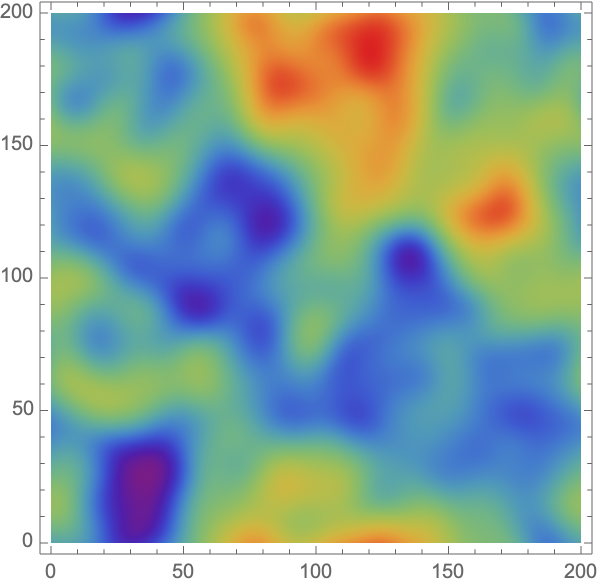
\includegraphics[width=\textwidth]{Psi}
\end{subfigure}~
\begin{subfigure}[b]{0.49\textwidth}
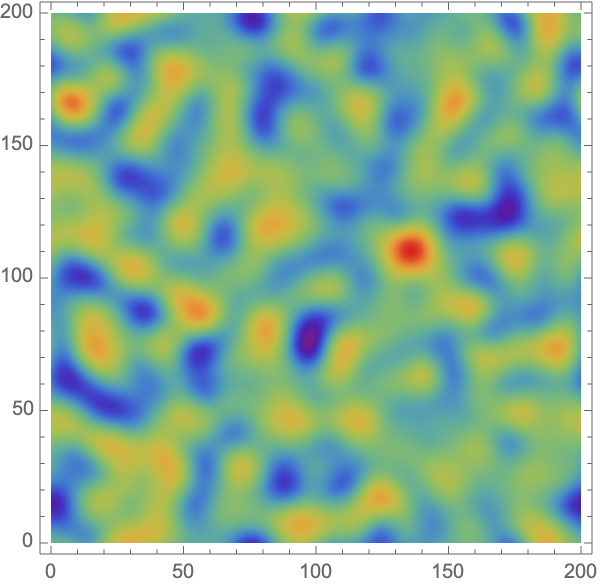
\includegraphics[width=\textwidth]{Rho}
\end{subfigure}\\
\begin{subfigure}[b]{0.49\textwidth}
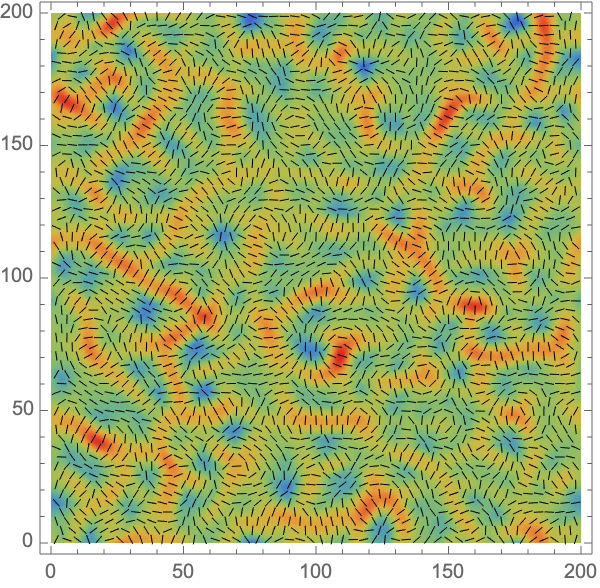
\includegraphics[width=\textwidth]{Lambda_1}
\end{subfigure}~
\begin{subfigure}[b]{0.49\textwidth}
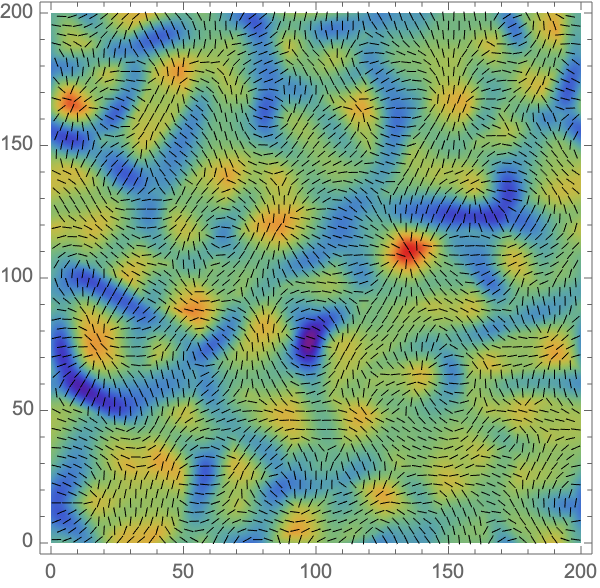
\includegraphics[width=\textwidth]{Lambda_2}
\end{subfigure}
\caption{A Gaussian random field and the corresponding eigenvalue and eigenvector fields. \textit{Upper left:} the initial gravitaitonal potential $\phi_0$. \textit{Upper right:} the corresponding density perturbation field $\delta$. \textit{Lower left:} the first eigenvalue and eigenvector fields $\mu_1,\bm{v}_1$. \textit{Lower right:} the second eigenvalue and eigenvector fields $\mu_2,\bm{v}_2$.}
\label{fig:Initial_Conditions}
\end{figure}

%%%%%%%%%%%%%%%%%%%%%%%%%%%%%%%%%%%%%%%%%%%%%%%%%%%%%%%%%%%%%%%%
\section{The caustic skeleton \& cosmic web illustrated}
\label{sec:Eulerian_space}
In this section, we describe the gravitational collapse of Gaussian fluctuations, the resulting emergence of an intricate cosmic network, known as the cosmic web, and the accurate and profound connection with the formation of caustic singularities in the mass distribution. The cosmic web -- consisting of voids, walls, filaments, and clusters -- is intimately tied to the development of multi-stream regions, which in turn are most naturally described in terms of caustics. These caustics capture the formation histories of the multi-stream regions and trace the spine of the cosmic web. Moreover, we point out a strong correspondence between the geometry of the eigenvalue fields of the initial deformation tensor (governed by the gravitational potential) and the geometry of the web at late times. 

In a first step towards elucidating and appreciating the intimate connection between the cosmic mass distribution in the cosmic web and its analytically predicted spine by the Caustic Skeleton model, we provide a visual impression of the primordial inhomogeneous matter distribution and corresponding inhomogeneous and anisotropic gravitational force field.

The present study limits itself to the treatment of the gravitationally evolving dark matter distribution in a two-dimensional setting. The development of the dark mark distribution in the corresponding four-dimensional phase-space can be seen as that of a gradually deforming two-dimensional {\it dark matter sheet} embedded in 4-D phase-space. For a visually direct assessment of the relation between the structural components of the cosmic web and the caustic singularities arising in the matter distribution, we confine our attention to the patterns observed in Eulerian space. 

The starting point for the emergence of the cosmic web is the primordial field of random Gaussian density and velocity fluctuations. The cosmic web is the product of the subsequent gravitationally propelled evolution. At each cosmic epoch, the mass distribution attains a weblike morphology at the scale at which the matter distribution evolves away from its initial linear evolution and nonlinear features start to appear as mass concentrations decouple from the Hubble expansion and start to contract gravitationally. At this quasi-linear phase, the migration streams involved in the buildup of the structure start to cross, and we see the emergence of multi-stream regions at the locations of the emerging nonlinear features. 

%%%%%%%%%%%%%%%%%%%%%%%%%%%%%%%%%%%%%%%%%%%%%%%%%%%%%%%%%%%%%%%%
\subsection{Caustics in the cosmological matter distribution}
\label{sec:primordial}
The cosmic mass distribution that we discuss in this section concerns the dark matter distribution in a two-dimensional realization in a box of $200 \mbox{Mpc}$ length. The cosmological background is a flat Einstein-de Sitter universe with a dark matter density $\Omega_m=1$ and Hubble constant $H_0=71\text{ Mpc/s/km}$. The structure evolves gravitationally out of a primordial Gaussian random field with a power-law power spectrum. The corresponding gravitational potential $\phi_0$ has a power-law spectrum $P_{\phi}(k) \propto k^{n_s}$, with a high-frequency cutoff at a smoothing scale $R_s$. For the present reference model the power law index $n_s=-1$ and the cutoff scale
$R_s=2.5 \text{ Mpc}$. The primordial field is generated on a $512^2$ grid.

The map of the Gaussian random potential field is shown in the top lefthand frame in figure~\ref{fig:Initial_Conditions}, with the corresponding map of the density field $\delta$ in the top righthand frame of the same figure. We use the Zel'dovich approximation's analytical expression for the deformation tensor to infer on the basis of the caustic conditions the nature of the caustic singularities that will arise in the evolving mass distribution \cite{Feldbrugge:2018}. The caustic conditions refer to the mass distribution in Lagrangian space, and they yield the Lagrangian location and outline of the various caustic singularities present in the generated mass distribution.  Table~\ref{table:caustics-cosmciweb} guides the morphological identity of the various caustic classes, for the two-dimensional situation. The full identification for the two- and three-dimensional situations can be found in \cite{Feldbrugge:2018}.

The primordial mass distribution is evolved to the current epoch ($z=0$). For the purpose of the present study, the evolution is followed in two ways. A two-dimensional dark matter $N$-body simulation \cite{Hidding:2020} is used to follow the fully nonlinear evolution of the mass distribution. This resulting nonlinear structure is discussed in section~\ref{sec:nbody}. In the Zel'dovich approximation, the Eulerian location and environment of these caustic features is obtained by using the corresponding expression for the displacement of a mass element. In the $N$-body simulation, their location follows from the simulation displacement of the corresponding mass elements (see figure~\ref{fig:Eulerian} and figure~\ref{fig:Eulerian_Evolution}).

\begin{table}
\centering
{\scriptsize
\begin{tabular}{ |l | l | l | l |}
  \hline
  \ && \\
\textbf{Caustic Singularity} & \textbf{Symbol} & \textbf{2D cosmic web}\\
\ && \\
\hline
\ && \\
Fold & $A_2$ & shell-crossing \\
Cusp & $A_3$ & filament \\
Swallowtail &$A_4$ &  cluster\\
Elliptic/hyperbolic & $D_4^{\pm}$ & cluster\\
Morse point & $A_3^+$ & creation/annihilation point\\
Morse point & $A_3^-$ & merger point\\
\ && \\
\hline
\end{tabular}
}
\caption{Elements of the two-dimensional caustic skeleton and their caustic conditions.}
\label{table:caustics-cosmciweb}
\end{table}

The direct comparison between the evolving $N$-body particle distribution allows us to assess the position and role of the various caustics within the cosmic mass distribution, and in particular that in the weblike network in which it has organized itself.

%%%%%%%%%%%%%%%%%%%%%%%%%%%%%%%%%%%%%%%%%%%%%%%%%%%%%%%%%%%%%%%%
\subsection{Primordial deformation field and cosmic web}
At the heart of the caustic conditions in \cite{Feldbrugge:2018} is the observation that the caustic singularities that are emerging in the matter distribution, and the structural weblike components surrounding them, are determined by the deformation and tidal field induced by the inhomogeneous mass distribution \cite{Zeldovich:1970,Weygaert:1996,Weygaert:2008,Hidding:2014}.

The key role of the eigenvalues of the deformation tensor in establishing the morphological nature of cosmic structure has been acknowledged since the seminal studies by \cite{Zeldovich:1970} and \cite{Doroshkevich:1970}. It formed the basis for the expectation that the cosmic mass distribution would be organized in a cellular pattern \cite[also see][]{Shandarin:1989,Shandarin:2009,sunyshand2014}. The instrumental role of the corresponding eigenvectors in establishing the overall structural pattern of the cosmic web, and its various components, was hardly acknowledged. The explicit demonstration by \cite{Feldbrugge:2018} revealed their importance in outlining the weblike structure.

The intimate connection between the deformation's eigenvalues and eigenvectors and the subsequent formation of the cosmic web is clearly revealed in the bottom panels of figure~\ref{fig:Initial_Conditions}. The panels provide a telling illustration of the central role of the deformation/tidal field tensor in establishing the spatial structure of the cosmic web that will emerge from these initial conditions as a result of gravitationally driven evolution. The map in the bottom lefthand panel represents the first eigenvalue $\lambda_1$ field and the bottom lefthand panel the second eigenvalue $\lambda_2$ field. The corresponding eigenvectors $\bm{v}_1$ and $\bm{v}_2$ are superimposed by means of black solid bars oriented along the eigenvector direction, depicted at a discrete number of grid locations. With respect to the eigenvector fields, we note that at initial times (\textit{i.e.}, in Lagrangian space), the eigenvector fields are normal, $\bm{v}_{t,1}\cdot \bm{v}_{t,2}=0$, since the deformation tensor is symmetric. The maps reveal that to a considerable extent a pervasive weblike network can already be recognized in the primordial deformation field. The eigenvalue and eigenvector maps are distinctly non-Gaussian fields, marking a highly structured pattern, with a high level of spatial coherence.

\begin{figure}
\centering
\begin{subfigure}[b]{0.49\textwidth}
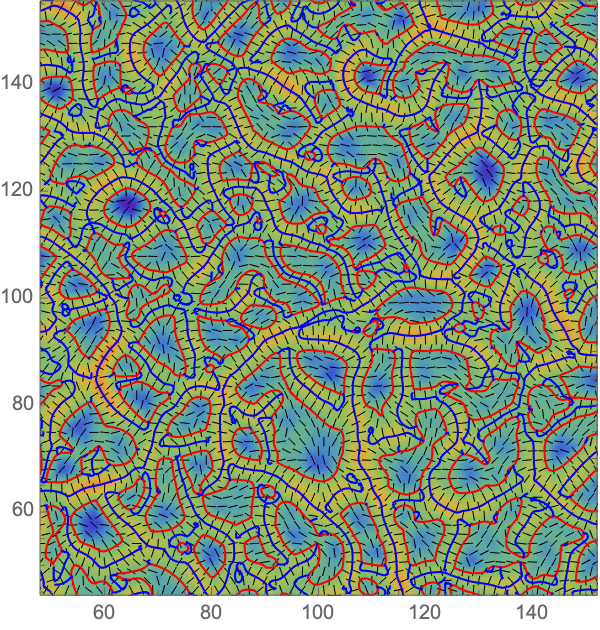
\includegraphics[width=\textwidth]{Eulerian_L}
\caption{$\lambda_1,\bm{v}_1$}
\end{subfigure}
\begin{subfigure}[b]{0.49\textwidth}
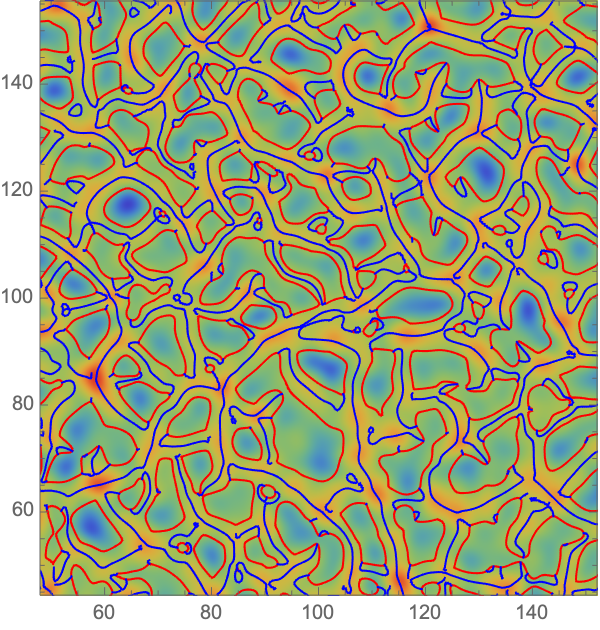
\includegraphics[width=\textwidth]{Eulerian_dens_old}
\caption{$\delta$}
\end{subfigure}\\[0.5cm]
\begin{subfigure}[b]{0.49\textwidth}
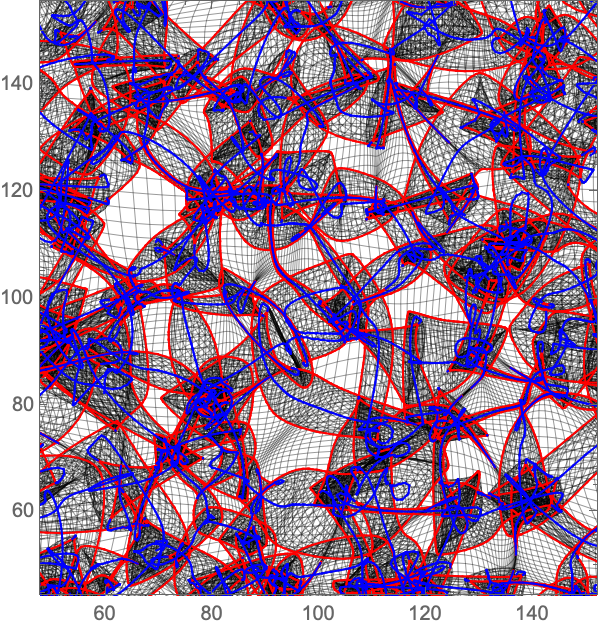
\includegraphics[width=\textwidth]{Eulerian_Z}
\caption{Zel'dovich approximation}
\end{subfigure}~
\begin{subfigure}[b]{0.49\textwidth}
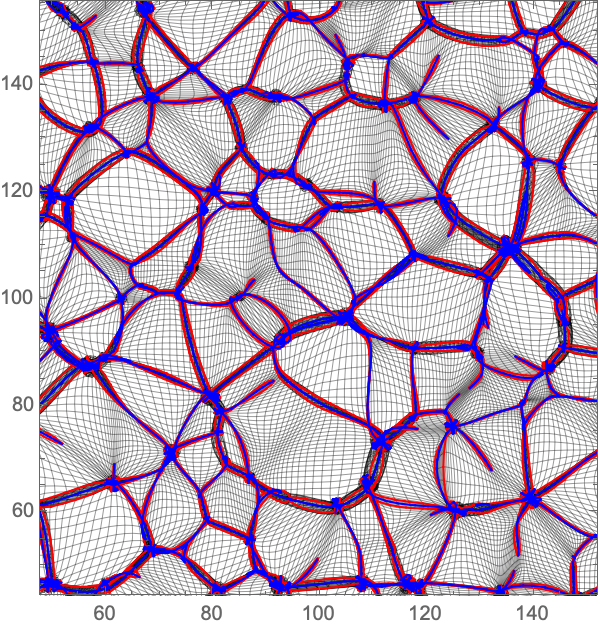
\includegraphics[width=\textwidth]{Eulerian_Nb}
\caption{$N$-body simulation}
\end{subfigure}
\caption{The caustic skeleton consisting of the $A_2$ fold curves (red) and $A_3$ cusp curve (blue) in Lagrangian and Eulerian space. \textit{Upper left (Lagrangian space):} the initial eigenvalue field $\lambda_1$ with the caustic skeleton. \textit{Upper right (Lagrangian space):} the initial density perturbation field, with the caustic skeleton superimposed. \textit{Lower left (Eulerian space):} the Zel'dovich approximation with the caustic skeleton at scale factor $a=1$ (Eulerian space). \textit{Lower right (Eulerian space):}  the $N$-body simulation with the caustic skeleton at scale factor $a=1$.}
\label{fig:Eulerian}
\end{figure}

%%%%%%%%%%%%%%%%%%%%%%%%%%%%%%%%%%%%%%%%%%%%%%%%%%%%%%%%%%%%%%%%
\subsection{Multistream regions and caustic skeleton}
Induced by the matter streams set into motion by the primordial inhomogeneous force field, spatially steered and directed by the corresponding deformation tensor orientation, matter starts to aggregate at locations where multiple streams meet up. The outline of these locations can already be recognized by the typically cellular patterns in the spatial primordial deformation eigenvalue distribution. Dependent on the precise nature and geometry of these multi-stream regions, \textit{i.e.}, the way in which the cosmic matter phase-space sheet is folded, we observe the formation and evolution of different characteristics components of the cosmic web. The nature of the complex spatial folding of the phase-space sheet in and around the flow field singularities determines the identity of the structural component of the cosmic web that arises in the spatial matter distribution.

The caustic conditions \cite{Feldbrugge:2018} allow us to infer exactly the location of the singularities in the matter distribution, the caustics. These conditions pertain to the nature and location of singularities in Lagrangian space. It means that at any cosmic epoch, the caustic conditions identify the mass elements that are included in a caustic singularity, for any of the possible caustic classes. Locating these mass elements at any subsequent cosmic epoch, by projecting them to their Eulerian position, yields the spatial outline of the spine of the cosmic web at that epoch. This spine is the assembly of the caustic membranes, ridges, and nodes around which matter organizes itself into the cosmic web. In other words, the set of analytical expressions for the caustic conditions represents a fully analytical description of the caustic skeleton of the cosmic web, and hence of its formation and evolution. Around this, a fully analytical theory of cosmic web formation can be formulated. The present study entails a major step in this program. 

\bigskip
The top panels of figure~\ref{fig:Eulerian} present a telling illustration of the intimate connection between the eigenvalue and eigenvector fields of the deformation tensor and the spatial outline of the various caustic singularities. The eigenvector field is represented by black directional bars along the direction of eigenvectors, depicted at a discrete number of grid locations. The top lefthand panel of figure~\ref{fig:Eulerian} captures the geometry of the first eigenvalue $\lambda_1$ field, along with the corresponding eigenvector $\bm{v}_1$ field.   Also interesting for our discussion is the observation that the eigenvector fields exhibit an interesting correlation with the eigenvalue fields. Roughly speaking, the eigenvector fields are normal to the ridges of the corresponding eigenvalue fields.

Both the $A_2$ fold (red) and $A_3$ cusp caustic curves (blue) are superimposed on the eigenvalue and eigenvector maps in figure~\ref{fig:Eulerian}. The red fold curves provide a reasonable approximation of the boundaries of multi-stream regions, which they enclose. Particularly interesting for understanding the connectivity of the cosmic web is the stringy network of (blue) cusp curves. At late times, they outline an interconnected network that bisects the multi-stream regions and forms knots at the clusters of the cosmic web. In other words, the ridges outlined by the cusp curves define the filamentary spine of the cosmic web. In addition, we see how blue (Lagrangian) regions bounded by the red fold curves are the progenitors of the voids: they delineate the mass elements that will remain in mono-stream regions. 

\begin{figure}
\centering
\begin{subfigure}[b]{0.49\textwidth}
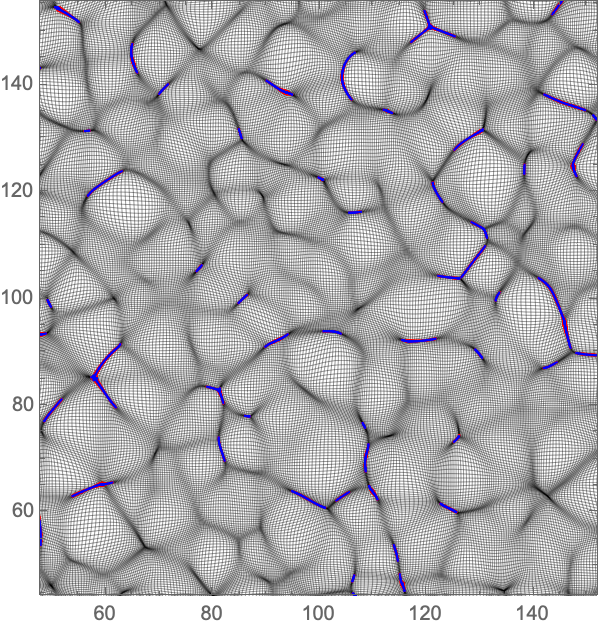
\includegraphics[width=\textwidth]{Evolution_020}
\caption{$a=0.2$}
\end{subfigure}~
\begin{subfigure}[b]{0.49\textwidth}
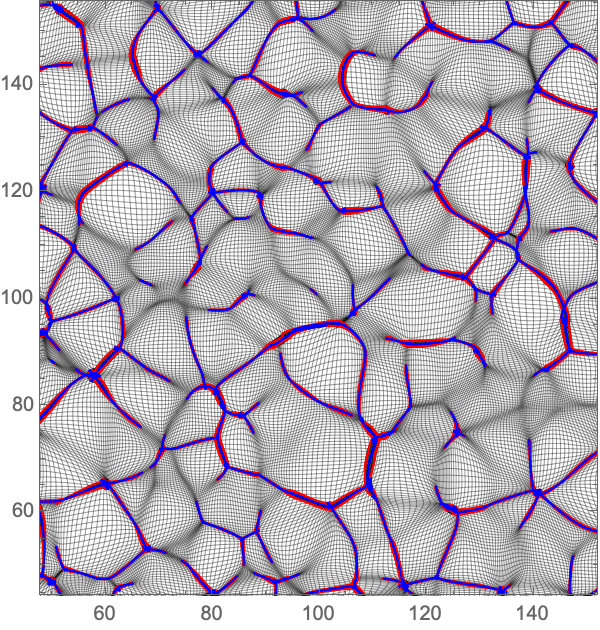
\includegraphics[width=\textwidth]{Evolution_040}
\caption{$a=0.4$}
\end{subfigure}\\[0.5cm]
\begin{subfigure}[b]{0.49\textwidth}
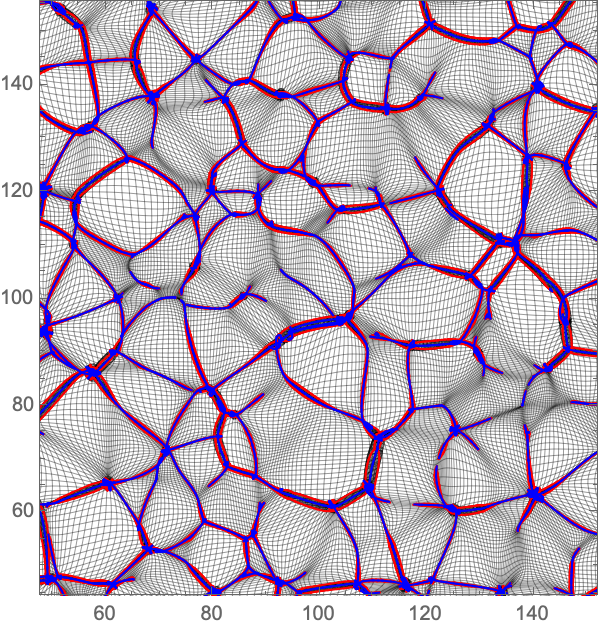
\includegraphics[width=\textwidth]{Evolution_060}
\caption{$a=0.6$}
\end{subfigure}~
\begin{subfigure}[b]{0.49\textwidth}
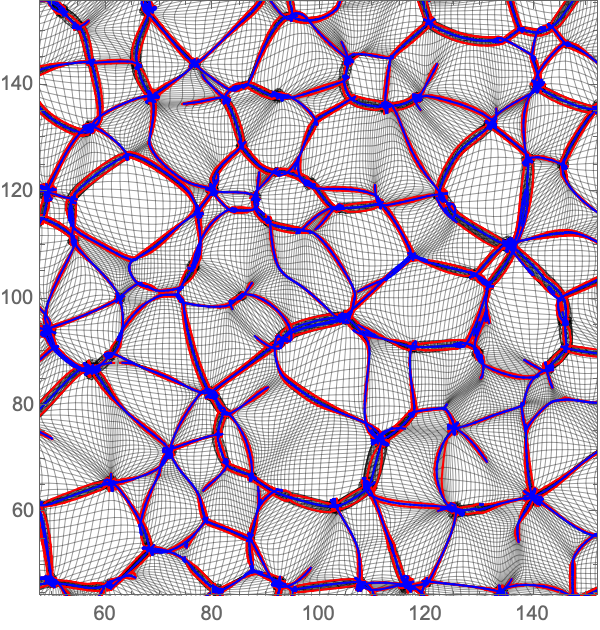
\includegraphics[width=\textwidth]{Evolution_080}
\caption{$a=0.8$}
\end{subfigure}
%\begin{subfigure}[b]{0.48\textwidth}
%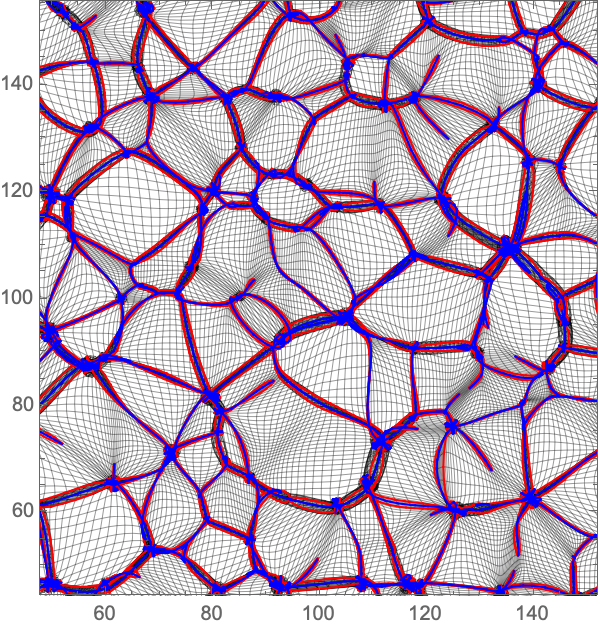
\includegraphics[width=\textwidth]{Evolution_100}
%\end{subfigure}
\caption{The evolution of the caustic skeleton consisting of the fold curves (red) and cusp curve (blue) in an $N$-body simulation in an Einstein-de Sitter universe. The skeleton for scale factor $a=1$ can be seen in the lower right panel of figure \ref{fig:Eulerian}.}
\label{fig:Eulerian_Evolution}
\end{figure}

\bigskip
The top righthand panel of figure~\ref{fig:Eulerian} compares the primordial density field with the caustic skeleton. At large scales, the eigenvalue field closely resembles the initial density perturbation $\delta_0 \propto \nabla^2\phi_0$. At these scales, the caustic skeleton follows the geometry of the super-level sets of the density perturbation. However, on intermediate to small scales, noticeable and significant qualitative differences appear. 

The red overdense regions in the primordial density field experience an inflow of matter. These lead to the emergence of the first caustics in and around these locations. Meanwhile, in and around the underdense blue regions we see the outflow of matter and the appearance of the first voids. When comparing the primoridal density field with the primordial second eigenvalue field, we observe that the peaks and troughs in both fields largely coincide. However, significant differences and deviations between the density and eigenvalue field occur at the medium field levels. The eigenvalue fields emphasize line-like features that connect the high-density regions. These elongated features in the first eigenvalue field are the progenitors of the most prominent components of the cosmic web, the filaments. 

Within the context of Lagrangian fluid dynamics, we may appreciate the central role of the deformation field in establishing the weblike pattern of the cosmic web. Lagrangian fluid dynamics emphasizes the role of gradients $\nabla \bm{s}_t$ in the displacement field $\bm{s}_t$, whose eigenvalues describe the compression and dilation along the principal axes of mass elements. At early times, the deformation tensor $\nabla \bm{s}_t$ is proportional to the Hessian of the gravitational potential, $\nabla \bm{s}_t \propto \mathcal{H}\phi_0$. From the eigenequation, it follows that the eigenvalue fields are the quadratic (or cubic) roots of a polynomial whose coefficients depend on the first-order gradients of the displacement field. As a result, the eigenvalue fields are distinctly nonlinear. In fact, this nonlinearity captures part of the nonlinear dynamics of the corresponding gravitational evolution and collapse. It also translates into the distinct non-Gaussian stochastic character of the eigenvalue fields (and corresponding eigenvector fields), in turn, a reflection of the distinctly non-Gaussian weblike pattern that we already find back in the primordial eigenvalue fields (see figure~\ref{fig:Initial_Conditions}, bottom panels).

%%%%%%%%%%%%%%%%%%%%%%%%%%%%%%%%%%%%%%%%%%%%%%%%%%%%%%%%%%%%%%%%
\subsection{The Eulerian caustic skeleton}
\label{sec:nbody}
To develop a visual appreciation of the roles of the different caustics in the observed large-scale structure of the Universe, the most direct assessment is that based on the implied structure in Eulerian space. In the current study, the evolution is followed in two ways. The Zel'dovich approximation offers a -- first-order -- analytical expression for the displacement of all mass elements. By displacing the mass elements accordingly, we obtain the Eulerian location and outline of the various caustic features present in the evolved matter distribution.  A two-dimensional dark matter $N$-body simulation \cite{Hidding:2020} is used to follow the fully nonlinear evolution of the mass distribution. In the $N$-body simulation, their location follows from the simulation displacement of the corresponding mass elements. The bottom panels of figure~\ref{fig:Eulerian} show the implied Eulerian structure of two descriptions for the nonlinear evolution of structure. The bottom lefthand panel shows the structure implied by the Zel'dovich approximation, at the current cosmic epoch $z=0$, while the bottom righthand panel shows the structure
obtained through an $N$-body simulation. 

Both the Zel'dovich modeling as well as the $N$-body simulation involve a $512^2$ particle simulation, in a box of size $200 \mbox{Mpc}$, and evolve the primordial mass distribution specified in section~\ref{sec:primordial}. 

The bottom lefthand panel of figure~\ref{fig:Eulerian} illustrates immediately the failure of the Zel'dovich approximation to represent the evolving cosmic mass distribution. The approximation linearly extrapolates the initial flow of the mass elements and ignores any further change in the gravitational interactions. As a result, it leads to overshooting after shell-crossing. Nonetheless, even though the Zel'dovich approximation does not accurately predict the location of the multi-stream regions and density fields at advanced evolutionary stages, it does manage to accurately predict the locations and times at which mass elements undergo shell-crossing and form caustics in Lagrangian space at these late times.

The comparison with the resulting weblike matter distribution of the $N$-body simulation, in the bottom righthand panel, however, reveals the high level of accuracy with which the predicted caustic skeleton delineates the mass distribution. The fold curves ($A_2$, red) provide a reasonable approximation of the boundaries of the multi-stream regions. Meanwhile, the cusp curves ($A_3$, blue) neatly bisect the multi-stream regions and form knots in the clusters of the cosmic web. With respect to the latter, we should appreciate that a cluster rarely consists of a single cluster caustic. Instead, the related caustics are correlated and combine to form at the knots an intertwined and intricate set of multi-stream curves. Filaments, on the other hand, experience a more organized development. As a result, they are usually associated with a single and unique cusp curve. 

%%%%%%%%%%%%%%%%%%%%%%%%%%%%%%%%%%%%%%%%%%%%%%%%%%%%%%%%%%%%%%%%
\subsection{The evolving caustic skeleton}
The evolving structure of the cosmic web, and its diverse structural components, can be followed systematically by following the corresponding development of the different caustic features through cosmic time. Figure \ref{fig:Eulerian_Evolution} provides a timeline for the resulting development of the $A_2$ fold curves and the $A_3$ filamentary cusp curves of the cosmic web at 4 cosmic epochs ($a=0.2$, $a=0.4$, $a=0.6$ and $a=0.8$). On the mass distribution followed by an $N$-body simulation (black), we find superimposed the red fold lines, indicating the location of the mass elements entering a multi-stream region, and the blue cusp lines, indicating the filamentary spine of the cosmic web. 

The multi-stream regions of the cosmic web, and the corresponding caustic features, form and evolve gradually. At early times, the {\it dark matter sheet} consists of a single single-stream region. As the mass elements undergo gravitational contraction and collapse, we observe the formation of several Zel'dovich pancakes corresponding to the maxima of the eigenvalue field $\lambda_1$ (see also figure~\ref{fig:Eulerian}, upper left panel). These multi-stream regions grow and connect at the saddle points of the eigenvalue fields to form the web-like structure we observe in redshift surveys (see the upper right and lower panels).

From the evolutionary sequence in figure~\ref{fig:Eulerian_Evolution} we observed that fully contracted filaments move coherently, while the large voids expand and the smaller voids contract. The latter is a key aspect of the hierarchical buildup of the void population \cite[see][]{Sheth:2004}. Also, the filamentary ridge of the cosmic web builds up hierarchically, with several filaments merging while forming more massive filaments. By concentrating on the evolution of the (blue) cusp curves, we can follow this process in detail. Filaments merge at $A_4$ swallowtail junctions, revealing the details of the process in which the connectivity of the various cosmic web elements is established. Because of the explicit analytical expressions for this process in terms of the corresponding caustic condition for $A_4$ caustics, we are handed a full and explicit analytical description of the hierarchical establishment of the complex connectivity of the cosmic web.

%%%%%%%%%%%%%%%%%%%%%%%%%%%%%%%%%%%%%%%%%%%%%%%%%%%%%%%%%%
\section{The caustic skeleton in Lagangian space}\label{sec:Caustic_Skeleton_Theory}
While a Lagrangian fluid evolves, it may develop singular features known as caustics. These caustic are fully classified by Lagrangian catastrophe theory and play an important role in the development of the cosmic web. In this section, we give an elementary description of Lagrangian fluid dynamics and summarize the highlights of caustic skeleton theory in two dimensions. In the present section, we develop the mathematical formalism underlying the Caustic Skeleton. It summarizes the extensive -- Lagrangian -- formalism outlined in \cite{Feldbrugge:2018}. Here we present the specific formulation of the caustic conditions in terms of the 2D eigenvalues and eigenvectors of the deformation tensor, providing the language for the development of the nonlinear constraint formalism for the various caustic classes.

The gravitational evolution, contraction, and collapse of density fluctuations in an expanding universe may be described from various perspectives. Most treatments follow the Eulerian perspective. The evolution of density, velocity, and gravitational potential of the matter fluid are considered in terms of a localized description of these quantities. The -- local mean -- density, velocity, and potential, evolve as described by the equation for the conservation of mass, the equation of motion through the Euler equation, and the Poisson equation for the potential corresponding to the density distribution. The Eulerian formalism is concise and leads to a reasonably accurate description of the mean flow in a large fraction of space.

Because the Eulerian description concerns local mean quantities, it is not able to describe the multi-stream nature of cosmic flow fields. To be able to describe cosmic flow fields consisting of several mass streams, each with its own distinct mass content and velocity, a Lagrangian formalism offers a powerful and natural alternative for the description of the dynamics of the evolving cosmic matter distribution. 

%%%%%%%%%%%%%%%%%%%%%%%%%%%%%%%%%%%%%%%%%%%%%%%%%%%%%%%%%%%%%%%%
\subsection{Lagrangian fluid dynamics}
The Lagrangian formalism models the matter fluid in terms of a collection of mass elements uniformly filling space at the initial time. Subsequently, it follows the path and evolving physical properties of the individual mass elements. Identifying each mass element by its initial -- Lagrangian -- position $\bm{q}$, its path is specified in terms of its displacement $\bm{s}_t(\bm{q})$. The evolving spatial distribution of mass elements is then captured by the Lagrangian map $\bm{x}_t:\mathcal{L}\to \mathcal{E}$,
\begin{align}
\bm{x}_t(\bm{q}) = \bm{q} + \bm{s}_t(\bm{q})\,.
\end{align}
The Lagrangian map describes the position of a mass element starting from the position $\bm{q}$ in Lagrangian space $\mathcal{L}$ to the final position $\bm{x}_t(\bm{q})$ at time $t$ in Eulerian space $\mathcal{E}$, with the displacement field $\bm{s}_t(\bm{q})= \bm{x}_t(\bm{q}) - \bm{q}$. Each mass element can flow, stretch, and rotate while conserving its mass. The density of a Lagrangian fluid is derived from the Lagrangian map through the conservation of mass, \textit{i.e.},
\begin{align}
\rho_t(\bm{x})
&= \sum_{\bm{q} \in A_t(\bm{x})} \frac{\bar{\rho}}{|\det \nabla \bm{x}_t(\bm{q})|}\nonumber\\
&= \sum_{\bm{q} \in A_t(\bm{x})} \frac{\bar{\rho}}{|1+\mu_{t,1}(\bm{q})||1+\mu_{t,2}(\bm{q})|}\,,
\label{eq:density}
\end{align}
with the mean initial density $\bar{\rho}$, and the eigenvalue fields $\mu_{t,1}$ and $\mu_{t,2}$ of the deformation tensor $\nabla \bm{s}_t$, defined by the eigenequation
\begin{align}
\nabla \bm{s}_t(\bm{q}) \bm{v}_{t,i}(\bm{q}) = \mu_{t,i}(\bm{q}) \bm{v}_{t,i}(\bm{q})\,,
\label{eq:EigenvalueAndEigenvector}
\end{align} 
with the corresponding eigenvector fields $\bm{v}_{t,1}$, and $\bm{v}_{t,2}$. Each stream contributes to the density, as the sum runs over the points that reach $\bm{x}$ in time $t$, \textit{i.e.},
\begin{align}
A_t(\bm{x}') = \{\bm{q}\,|\,\bm{x}_t(\bm{q})=\bm{x}'\}\,.
\end{align} 
Lagrangian fluid dynamics is well-known to be an effective tool to model the cosmic web, as demonstrated by the famous Zel'dovich approximation \cite{Zeldovich:1970}, second-order Lagrangian perturbation theory ($2$LPT) \cite{Buchert:1992, Buchert:1993a, Buchert:1993b, Buchert:1994a, Buchert:1994b, Bouchet:1995}, and $N$-body simulations \cite{Springel:2005, illustris:2014, eagle:2015, ABACUSSUMMIT:2021, Quijote:2020}. 

A two-dimensional Lagrangian fluid forms a two-dimensional sheet $M_t=\{(\bm{q},\bm{x}_t(\bm{q})) \, |\, \bm{q}\in \mathcal{L}\}$ in four-dimensional \textit{phase-space} $\mathcal{L}\times \mathcal{E}$, consisting of the inital and the final positions of the mass elements. Note that there exists a direct correspondence between this definition of phase-space and the more conventional phase-space consisting of the position and momentum of a particle in Hamiltonian mechanics. The cosmic web emerges in the projection of the phase-space sheet $M_t$ onto the final position $\varphi:\mathcal{L}\times \mathcal{E} \to \mathcal{E}$, defined by the map $(\bm{q},\bm{x}) \mapsto\bm{x}$ (see figure \ref{fig:Phase-Space} for an illustration).
\begin{figure}
\centering
\begin{subfigure}[b]{0.49\textwidth}
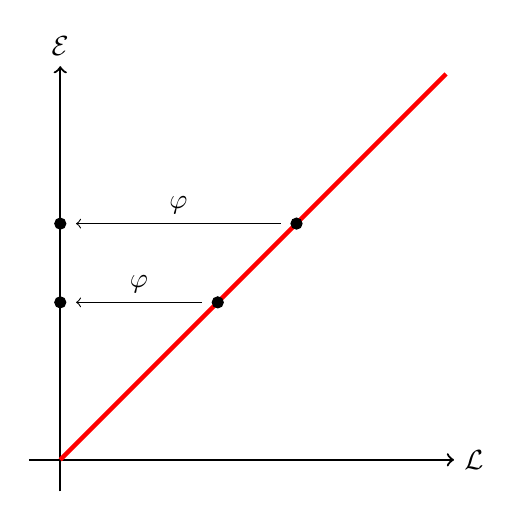
\begin{tikzpicture}
%\draw[help lines, color=gray!30, dashed] (-0.9,-0.9) grid (4.9,4.9);
\draw[->, thick] (-0.4,0)--(5,0) node[right]{$\mathcal{L}$};
\draw[->, thick] (0,-0.4)--(0,5) node[above]{$\mathcal{E}$};
\draw[-,ultra thick, red] (0,0)--(4.9,4.9);
\filldraw[black] (2,2) circle (2pt);
\filldraw[black] (0,2) circle (2pt);
\filldraw[black] (3,3) circle (2pt);
\filldraw[black] (0,3) circle (2pt);
\draw[->] (1.8,2) -- node[above] {$\varphi$} ++ (-1.6,0);
\draw[->] (2.8,3) -- node[above] {$\varphi$} ++ (-2.6,0);
\end{tikzpicture}
\end{subfigure}~
\begin{subfigure}[b]{0.49\textwidth}
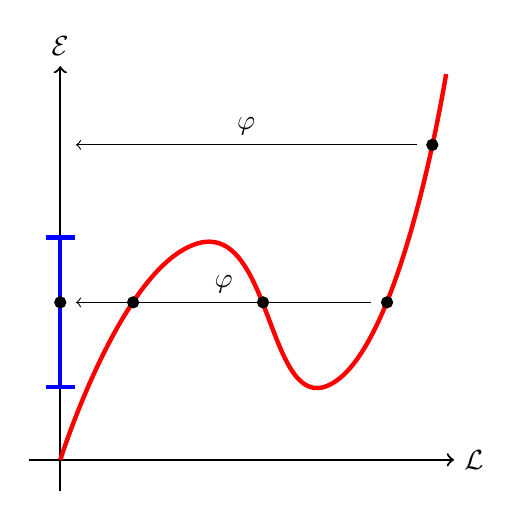
\begin{tikzpicture}
%\draw[help lines, color=gray!30, dashed] (-0.9,-0.9) grid (4.9,4.9);
\draw[->, thick] (-0.4,0)--(5,0) node[right]{$\mathcal{L}$};
\draw[->, thick] (0,-0.4)--(0,5) node[above]{$\mathcal{E}$};
\draw[|-|,ultra thick, blue] (0,0.9)--(0,2.85);
\draw [-, ultra thick, red] plot [smooth, tension=1] coordinates { (0,0) (1.75,2.75)  (3.5,1) (4.9,4.9)};
\filldraw[black] (0,2) circle (2pt);
\filldraw[black] (0.925,2) circle (2pt);
\filldraw[black] (2.575,2) circle (2pt);
\filldraw[black] (4.15,2) circle (2pt);
\filldraw[black] (4.725,4.) circle (2pt);
\draw[->] (3.95,2) -- node[above] {$\varphi$} ++ (-3.75,0);
\draw[->] (4.525,4.) -- node[above] {$\varphi$} ++ (-4.325,0);
\end{tikzpicture}
\end{subfigure}
\caption{Projection of phase-space to Eulerian space. The left panel illustrates the initial dark matter sheet in phase-space. The arrow represents the projection to Eulerian space $\varphi$. \textit{Left:} the initial dark matter sheet for which the mapping $\varphi$ is one-to-one. \textit{Right:} an evolved dark matter sheet consisting of a single- and a triple-stream region (in blue). Each point in the triple-stream region corresponds to three points on the dark matter sheet. The triple-stream region is bounded by a fold caustic at which the mass elements shell-cross.}\label{fig:Phase-Space}
\end{figure}
Initially, the displacement field vanishes, $\bm{s}_0(\bm{q})=\bm{0}$, and the phase-space manifold is diagonal $M_0=\{(\bm{q},\bm{q})\,|\,\bm{q} \in \mathcal{L}\}$. The mapping $\varphi$ is one-to-one, corresponding to a single-stream region (see the left panel of figure\ \ref{fig:Phase-Space}). When the fluid evolves, the phase-space manifold can develop complex configurations at which the mapping $\varphi$ becomes many-to-one, \textit{i.e.}, a final position can be reached from multiple initial positions. A connected region, in Eulerian space, with $n$ possible initial positions is known as an $n$-stream region (see the triple-stream region in the right panel of figure \ref{fig:Phase-Space}). In these multi-stream regions, gravitational collapse becomes non-linear and viralized structures start to form. The multi-stream regions partition the universe into regions with distinct formation histories, based on the dynamics of gravitational collapse. The fold caustic bound the multi-stream regions. At a fold, the orientation of the mass elements flips in a process known as \textit{shell-crossing}. In this process, the deformation tensor is singular, $\det \nabla \bm{x}_t = 0$, and the density \eqref{eq:density} spikes to infinity. As we will show in the next section, higher-order caustics in multi-stream regions can be associated with the membranes, filaments, and clusters of the cosmic web. The single-stream regions correspond colloquially to the voids, where the evolution of the cosmic web is well described by Eulerian fluid dynamics. For recent investigations on the phase-space structure of the cosmic web and the identification of multi-stream regions in $N$-body simulations see \cite{Hahn:2007, Abel:2012, Shandarin:2012,  Feldbrugge:2014b, Ramachandra:2015, Ramachandra:2017, Shandarin:2019, Shandarin:2021}.

%%%%%%%%%%%%%%%%%%%%%%%%%%%%%%%%%%%%%%%%%%%%%%%%%%%%%%%%%%%%%%%%
\subsection{Caustics in Lagrangian fluids}
The study of the cosmic web in terms of multi-stream regions and Lagrangian catastrophe theory has a rich history, predating the developments of $N$-body simulations. Amazingly, by analyzing the geometry of the caustics emerging in Lagrangian fluid dynamics, Y.\ Zel'dovich, V.\ Arnol'd and collaborators successfully predicted the qualitative features of the cosmic web \cite{Arnold:1982a, Arnold:1982b, Shandarin:1983, Rozhanskii:1984, Shandarin:1989}. The large-scale structure is described in terms of a network of caustics, analogous to the light patterns emerging on the sea bed or the bottom of a swimming pool \cite{Berry:1977, Berry:1980, Feldbrugge:2019}. 

However, these studies were mainly restricted to two-dimensional models, as several technical problems inhibited the full treatment of the three-dimensional cosmic web. In a recent publication \cite{Feldbrugge:2018}, we solved these problems by formulating the \textit{shell-crossing condition} describing how a submanifold in $\mathcal{L}$ can develop a non-differentiable feature under the mapping $\bm{x}_t$. Given a submanifold $L \subset \mathcal{L}$, the mapping $\bm{x}_t(L)$ develops a non-differentiable point at time $t$ in $\bm{q}_c$ when there exists a non-zero vector tangent vector $\bm{T}$ in the tangent space of $L$ at $\bm{q}_c$ for which 
\begin{align}
(1+\mu_{t,i}(\bm{q}_c))\bm{v}_{t,i}^*(\bm{q}_c) \cdot \bm{T}=0
\label{eq:shellCrossingCondition}
\end{align}
for all $i=1,2$, with $\bm{v}_{i,t}^*$ the dual eigenvector field defined by the relation $\bm{v}_{t,i}\cdot \bm{v}_{t,j}^* = \delta_{ij}$. The shell-crossing condition indicates the key role of the eigenvalue $\mu_{t,i}$ and eigenvector fields $\bm{v}_{t,i}$ of the deformation tensor $\nabla \bm{s}_t$ over the density field in the development of multi-stream regions. Note that even at early times, the eigenvalue fields are non-Gaussian and show the web-like structure of the late-time multi-stream regions and mass distribution (see figure \ref{fig:Initial_Conditions}). Furthermore note that not only the eigenvalue fields but also the, often ignored, eigenvector fields (see for example \cite{Forero:2009}) play a central role in the shell-crossing condition and the definition of the higher-order caustics, tracing the filaments and clusters of the cosmic web.

The shell-crossing condition leads to a set of \textit{caustic conditions} describing the properties of the displacement field in the vicinity of the caustic that stably occur in nature (for a derivation of Lagrangian catastrophe theory see \cite{Arnold:1972, Arnold:1976, Poston:1978, Gilmore:1981, Kravtsov:1983, Arnold:1984, Arnold:2012a, Arnold:2012b}). When applying the shell-crossing condition to Lagrangian space, $L=\mathcal{L}$, we obtain the condition for the fold caustic $A_2$,
\begin{align}
1+\mu_{t,i}(\bm{q}_c)=0
\end{align}
for $i=1$ or $2$, marking the shell-crossing region at which the density spikes. The fold curve is independent of the eigenvector fields. The fold curve bounds the different multi-stream regions (see the red curves in figure \ref{fig:caustics_Examples_Big}).

The fold curve develops non-differentiable points in the cusp caustic $A_3$, when the fold curve in Lagrangian space is parallel to the corresponding eigenvector field, \textit{i.e.}, 
\begin{align}
1+\mu_{t,i}(\bm{q}_c)=0\,,\\
\bm{v}_{t,i}(\bm{q}_c) \cdot \nabla \mu_{t,i}(\bm{q}_c)=0\,,\label{eq:cuspCondition}
\end{align}
See the intersection of the red and blue curves in figure \ref{fig:caustics_Examples_Big}, where the tangent vector of the red line is parallel to the eigenvector field. The term $\bm{v}_{t,i} \cdot \nabla \mu_{t,i}$ arises in the shell-crossing condition \eqref{eq:shellCrossingCondition} with $L=A_2$, from the observation that the tangent vector of the fold curve $\bm{T}$ is normal to the gradient of the eigenvalue field $\nabla \mu_{t,i}$. Over time, the cusp point defines the cusp curve which is associated with the filaments of the cosmic web. See the blue curve in the first row of figure \ref{fig:caustics_Examples_Big} for an example of a fold curve and its relation to the filaments of the cosmic web. 

In turn, the cusp curve develops a non-differentiable point known as a swallowtail caustic $A_4$ when the cusp curve in Lagrangian space is parallel to the eigenvector field, \textit{i.e.},
\begin{align}
1+\mu_{t,i}(\bm{q}_c)=0\,,\\
\bm{v}_{t,i}(\bm{q}_c) \cdot \nabla \mu_{t,i}(\bm{q}_c)=0\,,\\
\bm{v}_{t,i}(\bm{q}_c) \cdot \nabla (\bm{v}_{t,i}(\bm{q}_c) \cdot \nabla \mu_{t,i}(\bm{q}_c)) = 0\,.
\end{align}
The swallowtail caustic only exists for an instance in time and marks the location of a cluster, highlighting the location where different cusp curves join (see the second row of figure \ref{fig:caustics_Examples_Big}). 

In addition to the swallowtail caustic, the Lagrangian fluid also develops point-like caustics when both eigenvalue fields lead to a spike in the density field. The points for which
\begin{align}
1+\mu_{t,1}(\bm{q}_c) =0\,,\\
1+\mu_{t,2}(\bm{q}_c) = 0\,,
\end{align}
are known as the umbilic caustics $D_4^\pm$. The umbilic caustics consist of the elliptic $D_4^+$ and hyperbolic caustics $D_4^-$, both related to the clusters of the cosmic web. The umbilic caustics mark the locations where the cusp curves corresponding to the first and the second eigenvalue fields join (see the third and fourth rows of figure \ref{fig:caustics_Examples_Big}). 


\begin{figure}
\centering
\begin{subfigure}[b]{0.28\textwidth}
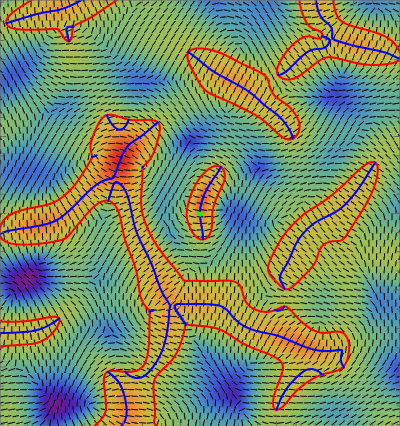
\includegraphics[width=\textwidth]{Cusp_L}
\end{subfigure}~
\begin{subfigure}[b]{0.28\textwidth}
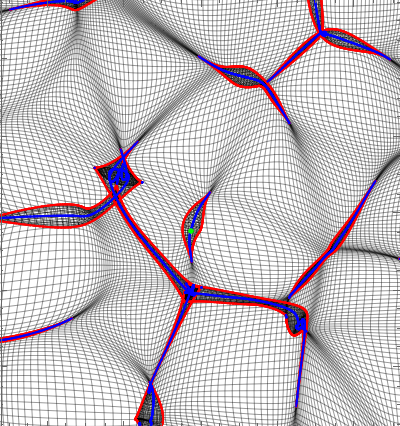
\includegraphics[width=\textwidth]{Cusp_Z}
\end{subfigure}~
\begin{subfigure}[b]{0.28\textwidth}
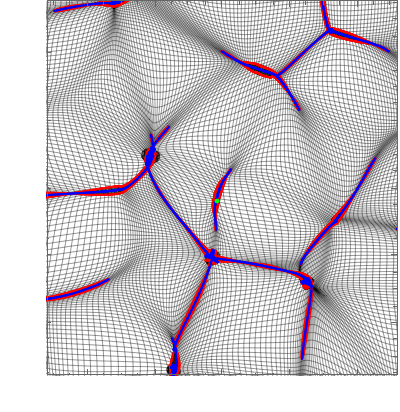
\includegraphics[width=\textwidth]{Cusp_Nb}
\end{subfigure}\\ \vspace{0.2\baselineskip}
%%%%%%%%%%
%%%%%%%%%%
\begin{subfigure}[b]{0.28\textwidth}
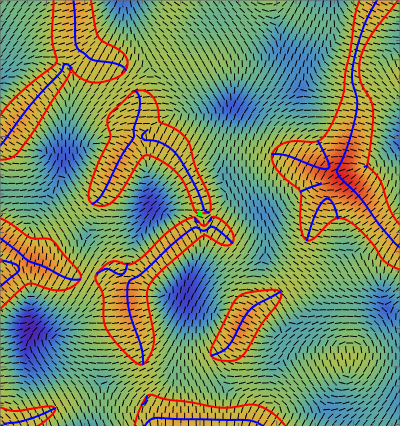
\includegraphics[width=\textwidth]{Swallowtail_L}
\end{subfigure}~
\begin{subfigure}[b]{0.28\textwidth}
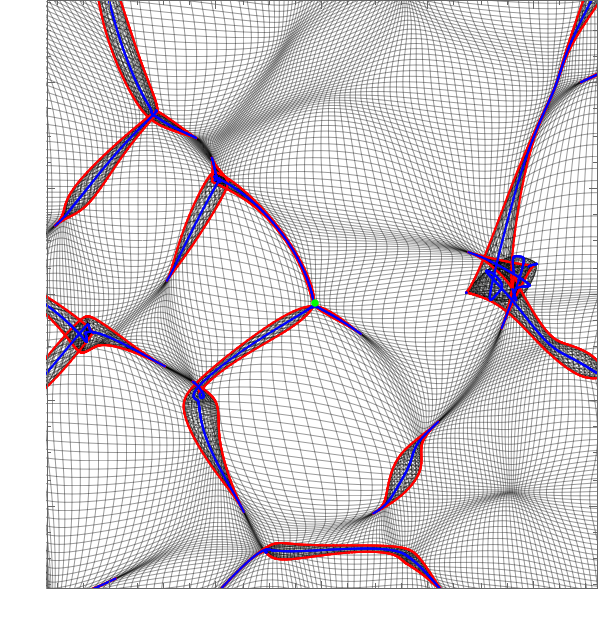
\includegraphics[width=\textwidth]{Swallowtail_Z}
\end{subfigure}~
\begin{subfigure}[b]{0.28\textwidth}
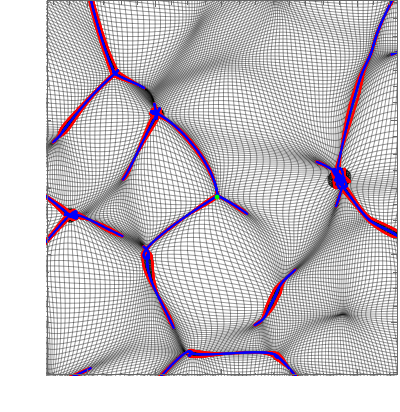
\includegraphics[width=\textwidth]{Swallowtail_Nb}
\end{subfigure}\\ \vspace{0.2\baselineskip}
%%%%%%%%%%
%%%%%%%%%%
\begin{subfigure}[b]{0.28\textwidth}
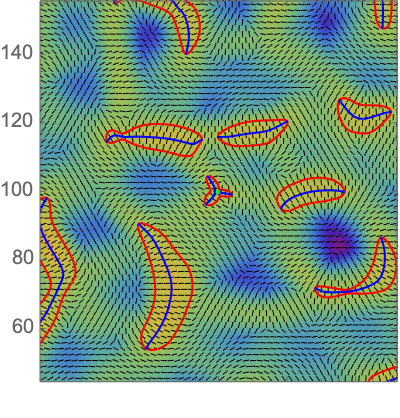
\includegraphics[width=\textwidth]{Elliptic_L}
\end{subfigure}~
\begin{subfigure}[b]{0.28\textwidth}
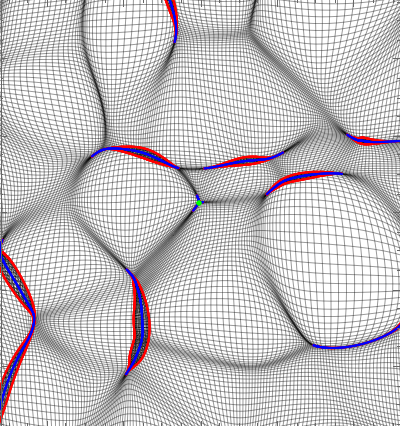
\includegraphics[width=\textwidth]{Elliptic_Z}
\end{subfigure}~
\begin{subfigure}[b]{0.28\textwidth}
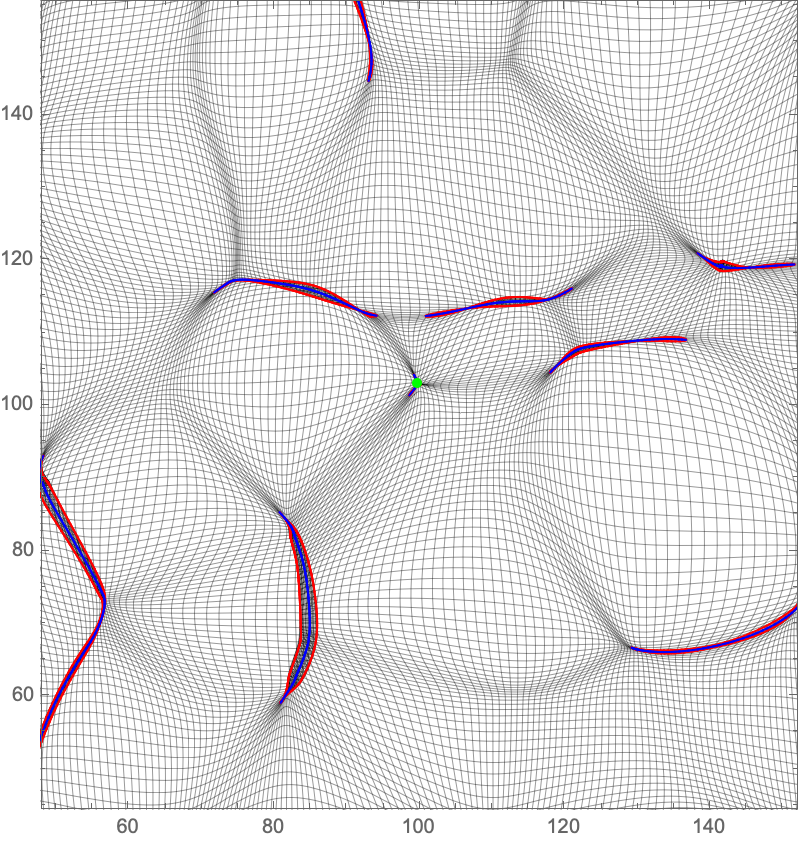
\includegraphics[width=\textwidth]{Elliptic_Nb}
\end{subfigure}\\ \vspace{0.2\baselineskip}
%%%%%%%%%%
%%%%%%%%%%
\begin{subfigure}[b]{0.28\textwidth}
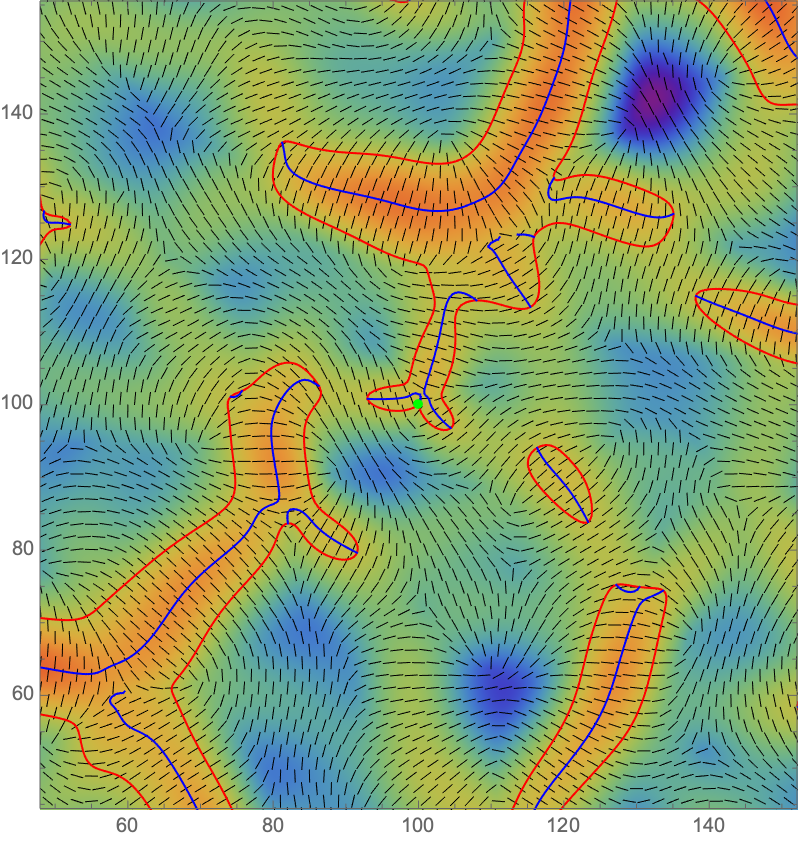
\includegraphics[width=\textwidth]{Hyperbolic_L}
\end{subfigure}~
\begin{subfigure}[b]{0.28\textwidth}
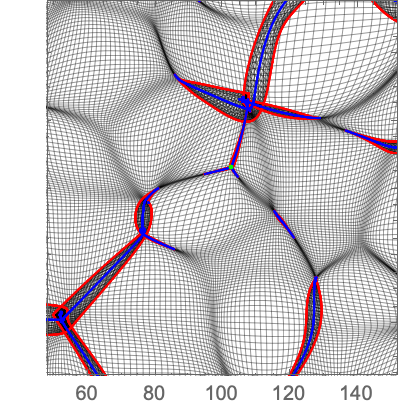
\includegraphics[width=\textwidth]{Hyperbolic_Z}
\end{subfigure}~
\begin{subfigure}[b]{0.28\textwidth}
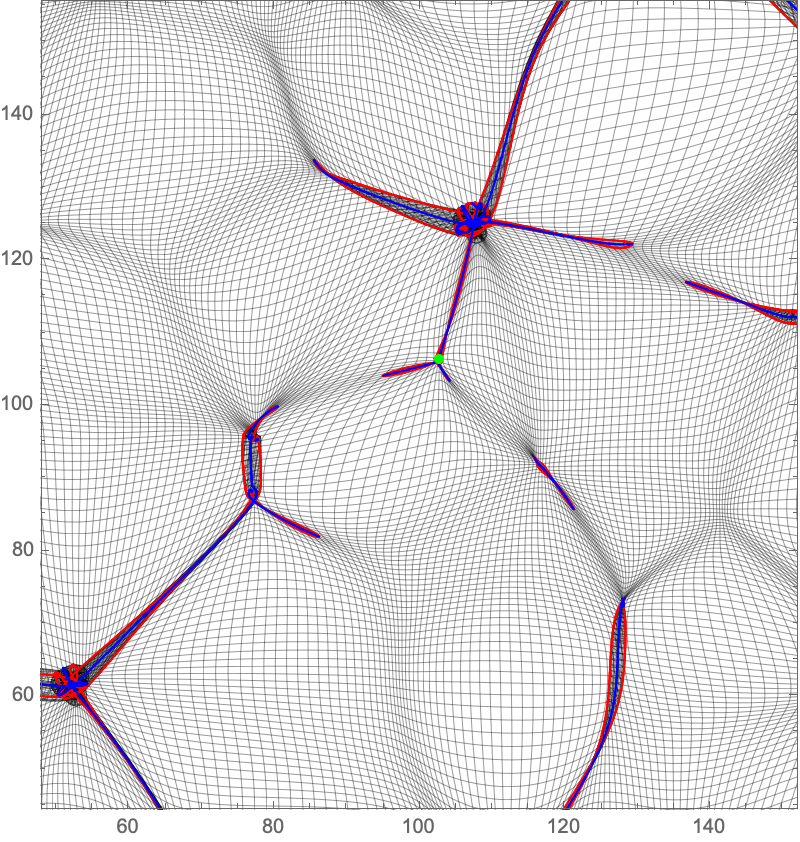
\includegraphics[width=\textwidth]{Hyperbolic_Nb}
\end{subfigure}
\caption{Elements of the caustic skeleton consisting of the fold curves (red) and cusp curve (blue) in Lagrangian and Eulerian space in a $[50\text{ Mpc}, 150 \text{ Mpc}]^2$ box. \textit{From top to bottom:} the cusp, the swallowtail, the elliptic, and the hyperbolic caustic. \textit{Left:} the caustic skeleton in Lagrangian space. \textit{Centre:} the Zel'dovich approximation. \textit{Right:} the corresponding $N$-body simulation \cite{Hidding:2020}.}\label{fig:caustics_Examples_Big}
\end{figure}




\begin{figure}
\centering
\begin{subfigure}[b]{0.24\textwidth}
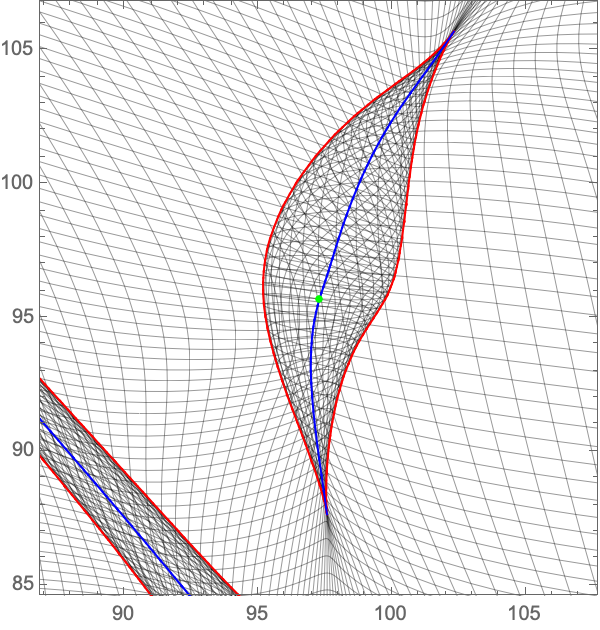
\includegraphics[width=\textwidth]{Cusp_Z_Zoom}
\end{subfigure}~
\begin{subfigure}[b]{0.24\textwidth}
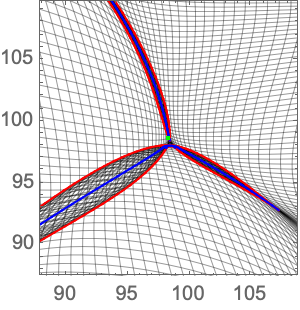
\includegraphics[width=\textwidth]{Swallowtail_Z_Zoom}
\end{subfigure}~
\begin{subfigure}[b]{0.24\textwidth}
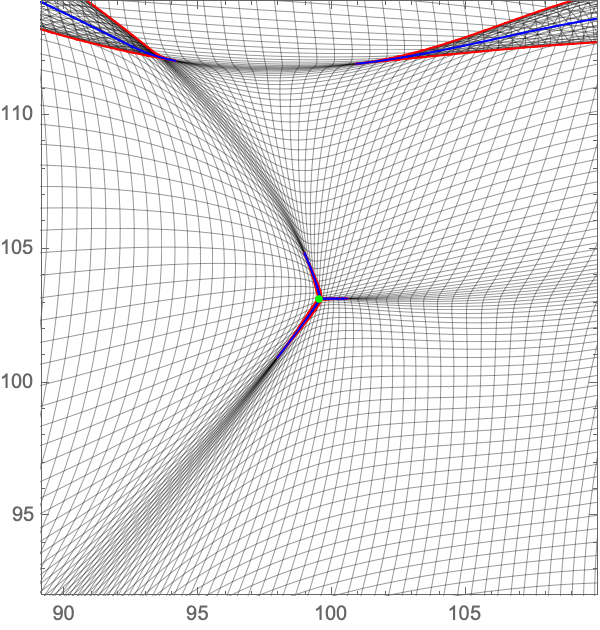
\includegraphics[width=\textwidth]{Elliptic_Z_Zoom}
\end{subfigure}~
\begin{subfigure}[b]{0.24\textwidth}
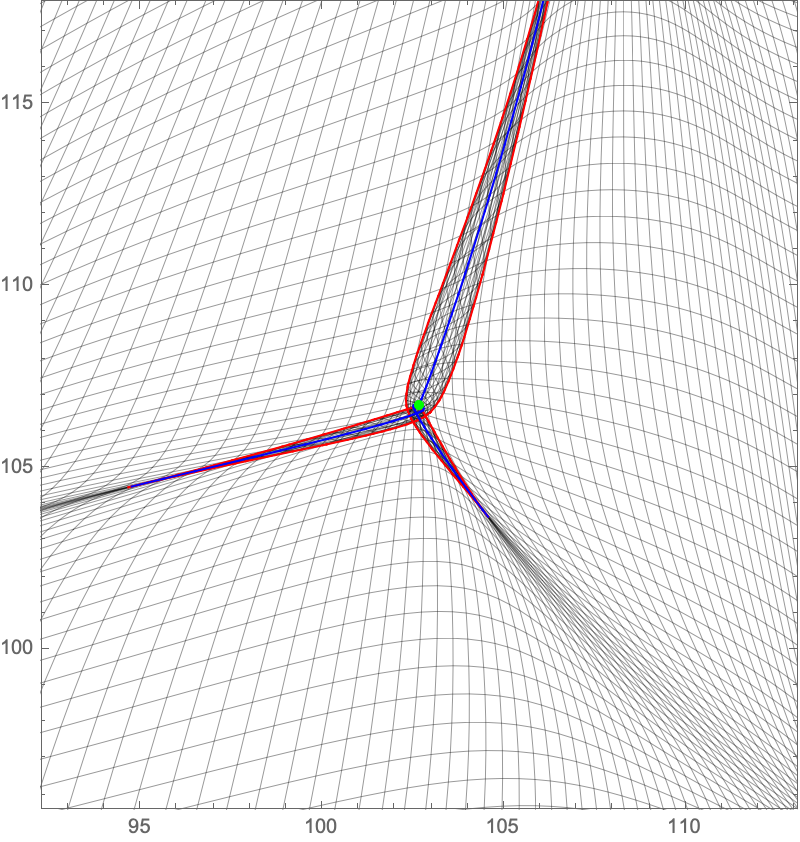
\includegraphics[width=\textwidth]{Hyperbolic_Z_Zoom}
\end{subfigure}\\
\begin{subfigure}[b]{0.24\textwidth}
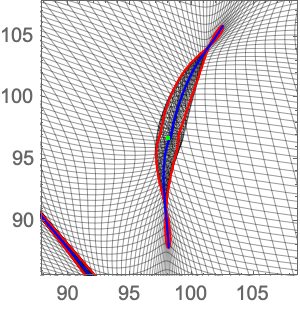
\includegraphics[width=\textwidth]{Cusp_Nb_Zoom}
\end{subfigure}~
\begin{subfigure}[b]{0.24\textwidth}
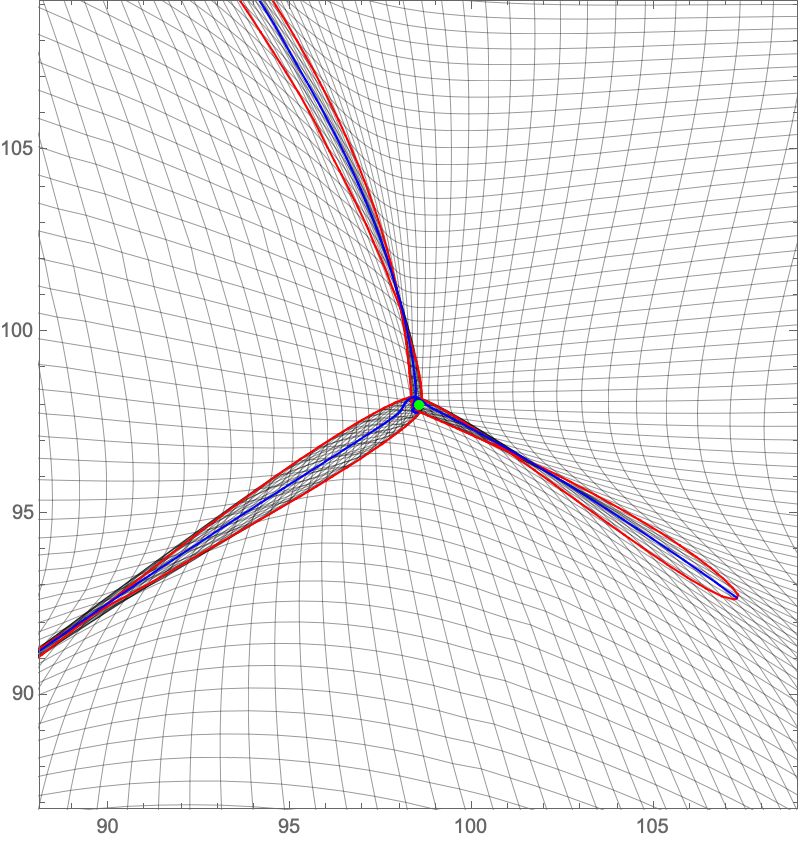
\includegraphics[width=\textwidth]{Swallowtail_Nb_Zoom}
\end{subfigure}~
\begin{subfigure}[b]{0.24\textwidth}
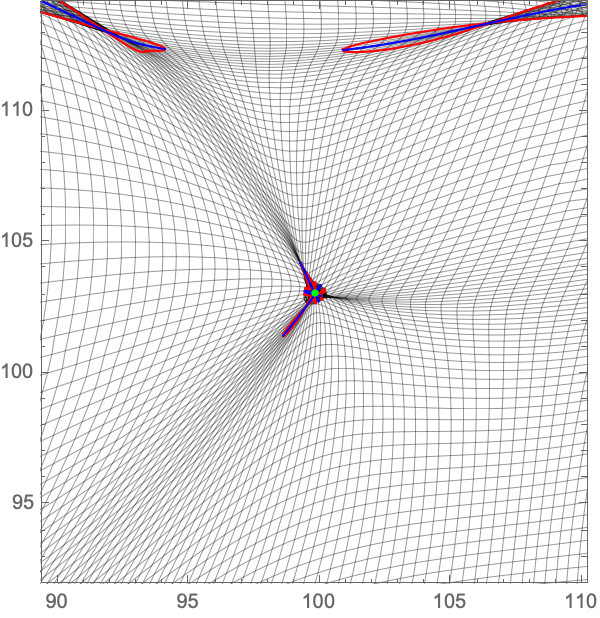
\includegraphics[width=\textwidth]{Elliptic_Nb_Zoom}
\end{subfigure}~
\begin{subfigure}[b]{0.24\textwidth}
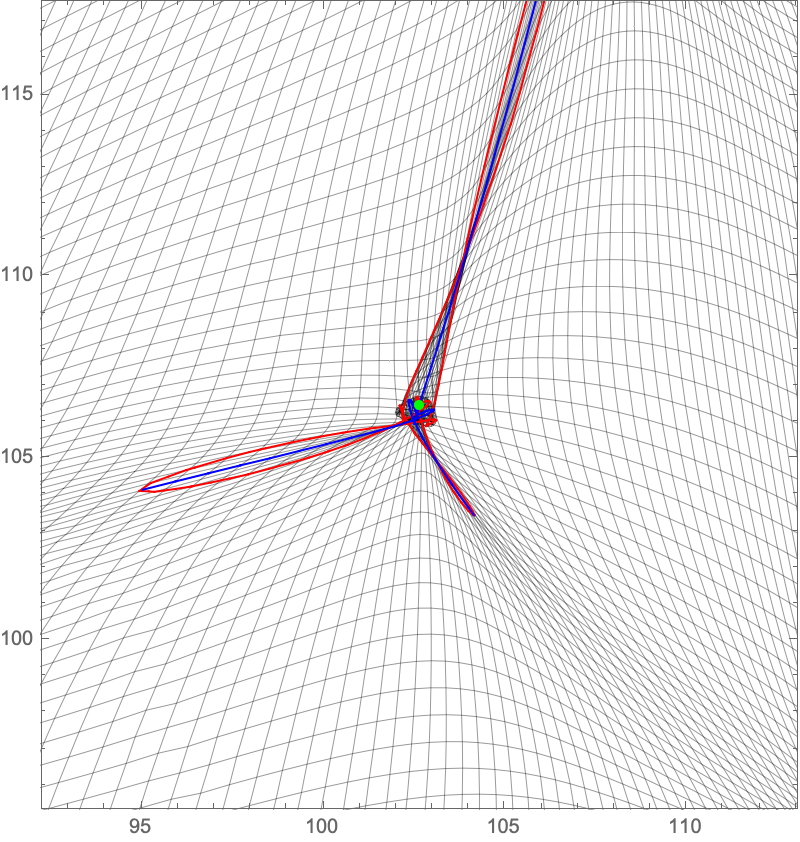
\includegraphics[width=\textwidth]{Hyperbolic_Nb_Zoom}
\end{subfigure}
\caption{Zoom in with a $(20 \text{ Mpc})^2$ box centered around the caustic, with the fold curve (red) and the cusp curve (blue). From left to right, we see the cusp, the swallowtail, the elliptic umbilic, and the hyperbolic umbilic caustics. The upper and lower panels display the Zel'dovich approximation and the $N$-body simulation \cite{Hidding:2020}.}\label{fig:caustics_Examples_Small}
\end{figure}

\begin{table}
\centering
{\scriptsize
\begin{tabular}{ |l | l | l | l | l|}
\hline
\textbf{Name} & \textbf{Symbol} & \textbf{2D cosmic web} & \textbf{Caustic conditions}\\
\hline
Fold & $A_2$ & shall-crossing & $1+ \mu_{t,i} = 0$ \\
\hline
Cusp & $A_3$ & filament & $1+ \mu_{t,i} = 0$, $\bm{v}_i \cdot \nabla \mu_{t,i} = 0$\\
\hline
Swallowtail &$A_4$ &  cluster & $1+ \mu_{t,i} = 0$, $\bm{v}_i \cdot \nabla \mu_{t,i} = 0,$ $\bm{v}_i \cdot \nabla(\bm{v}_i \cdot \nabla \mu_{i,t}) = 0$\\
\hline
Elliptic/hyperbolic & $D_4^{\pm}$ & cluster & $1+ \mu_{t,1} = 1+ \mu_{t,2} = 0$\\
\hline
Morse point & $A_3^+$ & creation/annihilation point& maximum/minimum of the eigenvalue field $\lambda_i$\\
\hline
Morse point & $A_3^-$ & merger point & saddle point of the eigenvalue field $\lambda_i$\\
\hline
\end{tabular}
}
\caption{Elements of the two-dimensional caustic skeleton and their caustic conditions.}
\label{table:caustics}
\end{table}



Finally, caustic skeleton theory includes a set of Morse points, at which the multi-stream regions emerge, vanish, and merge, changing the topology and connectivity of the cosmic web. The Morse points are defined as the critical points of the eigenvalue fields, satisfying the condition
\begin{align}
\nabla \mu_{t,i}(\bm{q}_c)=\bm{0}\,.
\end{align}
A critical point that undergoes shell-crossing always lies on a cusp curve, as a point with a vanishing gradient automatically satisfies equation \eqref{eq:cuspCondition}. The maxima and minima of the eigenvalue field $\mu_i$, known as $A_3^+$ points, mark the locations and times at which a multi-stream region forms or vanishes. The saddle point of the eigenvalue field $\mu_{t,i}$, known as $A_3^-$ points, mark the location and time at which two multi-stream regions merge to form a larger structure. The Morse points $A_3^-$ determine the connectivity of the cosmic web. We summarize the different elements of the caustic skeleton in table \ref{table:caustics}. For a complete contemporary description of caustic skeleton theory, we refer to \cite{Hidding:2014, Feldbrugge:2018}. 

See figure \ref{fig:caustics_Examples_Small} for a zoom-in of the various caustics in the Zel'dovich approximation and the $N$-body simulation. The fold line nicely bounds the multi-stream regions. The cusp curve bisects the multi-stream regions tracing the filaments. The swallowtail caustic and the umbilic caustics mark the knots where the filaments merge. Note that the caustic skeleton is evaluated for the Zel'dovich approximation and pushed to Eulerian space with either the Zel'dovich approximation or the $N$-body simulation. It is for this reason not surprising that the fold curve does not exactly match the shell-crossing region of the $N$-body simulation. Nevertheless, the caustics of the Zel'dovich approximation are very close to the caustics emerging in the fully non-linear model. Finally, note that the cluster caustics are in practice rarely isolated. The caustics cluster and together form a more intricate multi-stream structure. This way, a cluster can connect more than three filaments, even though the swallowtail and umbilic caustics individually connect only three filament regions.




\bigskip
Note that the study of the Morse points of the caustic skeleton has a direct connection to the DisPerSE and the Felix classification schemes \cite{Pogosyan:2009, Sousbie:2011a, Sousbie:2011b, Shivashankar:2016}, which apply Morse-Smale theory to the density field. In this scheme, the critical points of the density field connect the maxima via integral lines, which are associated with the filaments of the cosmic web. However, the caustic skeleton differs from Morse-Smale theory in several respects. Firstly, in this paper, we focus on the deformation tensor instead of the density field. The eigenvalue fields are non-Gaussian and tie into the dynamics of gravitational collapse. See figure \ref{fig:critical} for a comparison of the critical point densities of the initial density perturbation and the eigenvalue fields in the Zel'dovich approximation (see section \ref{sec:Zeldovich} for details). Secondly, the threshold of the caustic skeleton is determined by cosmic time (the growing mode for the Zel'dovich approximation). Finally, rather than connecting saddle points and maxima via integral lines satisfying a differential equation, the caustic skeleton connects the critical points using the simpler level sets \eqref{eq:cuspCondition} corresponding to the cusp caustic.



\begin{figure}
\centering
\begin{subfigure}[b]{0.32\textwidth}
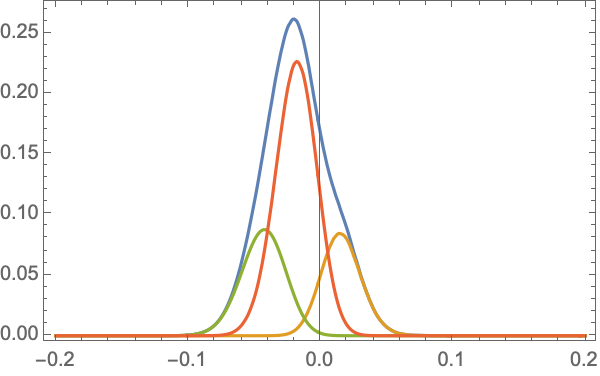
\includegraphics[width=\textwidth]{Critical_lambda_2}
\caption{The eigenvalue field $\mu_1$}
\end{subfigure}~
\begin{subfigure}[b]{0.32\textwidth}
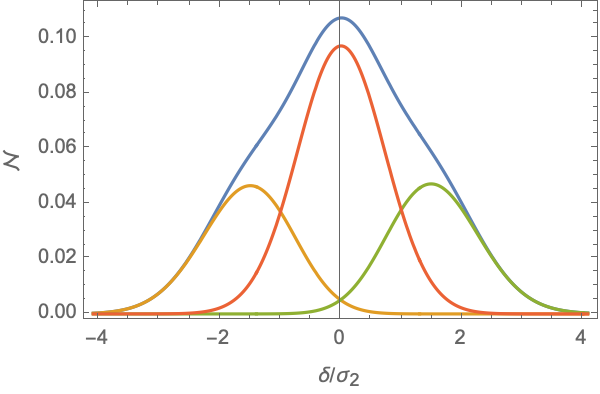
\includegraphics[width=\textwidth]{Critical_dens}
\caption{The density perturbation $\delta$}
\end{subfigure}~
\begin{subfigure}[b]{0.32\textwidth}
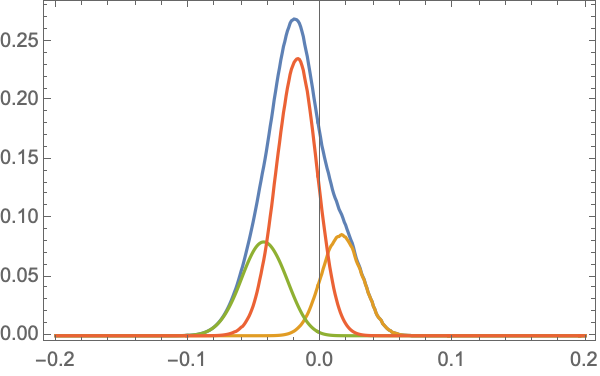
\includegraphics[width=\textwidth]{Critical_lambda_1}
\caption{The eigenvalue field $\mu_2$}
\end{subfigure}
\caption{The critical point densities of the density pertubation and the eigenvalue fields. The total critical point density (blue), the density of maxima (green), saddle points (red), and minima (orange).}\label{fig:critical}
\end{figure}
%%%%%%%%%%%%%%%%%%%%%%%%%%%%%%%%%%%%%%%%%%%%%%%%%%%%%%%%%%%%%%%%
\subsection{The Zel'dovich approximation}\label{sec:Zeldovich}
In this paper we define the caustic skeleton using the Zel'dovich approximation \cite{Zeldovich:1970} and study the resulting structures using a dark matter $N$-body simulation \cite{Hidding:2020}. The Zel'dovich approximation is the first-order approximation in Lagrangian fluid dynamics, for which the displacement field factorizes into a spatial and a temporal part
\begin{align}
\bm{s}_t(\bm{q}) = - b_+(t) \nabla_{\bm{q}} \Psi(\bm{q})\,.
\end{align}
The growing mode $b_+(t)$ is a natural time parameter, increasing monotonically, satisfying the differential equation
\begin{align}
\frac{\mathrm{d}^2 b_+(t)}{\mathrm{d}t^2} + 2 \frac{\dot{a}(t)}{a(t)} \frac{\mathrm{d} b_+(t)}{\mathrm{d}t} = 4 \pi G \rho_u(t) b_+(t)\,,
\end{align}
in terms of the scale factor $a$, the mean density $\rho_u = \langle \rho \rangle$, and Newton's gravitaitonal constant $G$. The displacement potential $\Psi$ captures the geometry of the cosmic web
\begin{align}
\Psi(\bm{q}) &=\frac{1}{4 \pi G a^2 \rho_0}\phi_0(\bm{q})%\\
%&= \frac{2}{3\Omega_0 H_0^2}\phi_0(\bm{q})
\,,
\end{align}
expressed in terms of the current total energy density %$\Omega_0$ and
$\rho_0$,
%the current Hubble parameter $H_0$,
and the linearly extrapolated gravitational potential $\phi_0$. The Poisson equation relates the primordial gravitational potential to the primordial density perturbation
\begin{align}
\nabla ^2 \phi_0 &= 4 \pi G a^2 \rho_u \delta_0\,,%\\
%&= \frac{3}{2} \Omega H^2 a^2 \delta\,,
\end{align}
with the dimensionless density contrast
\begin{align}
\delta(\bm{q}) = \frac{\rho(\bm{q})}{\rho_u} -1\,.
\end{align}
When working with the Zel'dovich approximation, it is convenient to work in terms of the Hessian of the displacement potential,
\begin{align}
\bm{\psi}=\mathcal{H}\Psi\,,
\end{align}
and the corresponding eigenvalue $\lambda_i$ and $\bm{v}_i$
\begin{align}
\bm{\psi}\bm{v}_i = \lambda_i \bm{v}_i\,,
\end{align} 
at early times satisfying the relation $\lambda_1 =-\mu_2/b_+,\lambda_2 =-\mu_1/b_+$. For convenience, we will assume the ordering $\lambda_1(\bm{q}) \geq \lambda_2(\bm{q})$ such that the first collapse corresponds to the first eigenvalue field $\lambda_1$. In terms of the eigenvalue fields $\lambda_i$, the density takes the form 
\begin{align}
\rho_t(\bm{x})
&= \sum_{\bm{q} \in A_t(\bm{x})} \frac{\bar{\rho}}{|1-b_+(t) \lambda_1(\bm{q})||1-b_+(t) \lambda_2(\bm{q})|}\,.
\end{align}
Initially, the growing mode $b_+$ vanishes and the universe consists of a single-stream region. As the fluid collapses under self-gravity, the growing mode $b_+$ increases. The fold caustics form at the level sets of the eigenvalue field $\{\bm{q}\,|\,\lambda_i(\bm{q})=1/b_+(t)\}$. From this picture, we observe the direct connection between the critical points of the eigenvalue fields and the connectivity of the cosmic web through Morse theory.

As described in the previous section, the eigenvalue fields of the deformation tensor are non-Gaussian. From the Poisson equation, it follows that the sum of the eigenvalue fields is proportional to the initial density contrast $\lambda_1+\lambda_2 \propto \delta_0$ and the joint probability distribution is given by the two-dimensional Doroshkevich formula \cite{Doroshkevich:1970, Feldbrugge:2014}
\begin{align}
p(\lambda_1,\lambda_2) = \frac{2\sqrt{2}}{\sqrt{\pi} \sigma_2^3} e^{-\frac{3(\lambda_1+\lambda_2)^2-8\lambda_1 \lambda_2}{2 \sigma_2^2}}|\lambda_1-\lambda_2|\,,
\end{align}
(see figure \ref{fig:eigen_stats}), with $\sigma_2$ the generalized moment defined in section \ref{sec:GRF}.


The Zel'dovich approximation describes the evolution of mass elements in terms of ballistic motion. The mass elements follow linear trajectories determined by the primordial gravitational potential. The approximation accurately describes single-stream regions at early times but fails at late times in multi-stream regions when gravitational backreaction of the mass elements becomes important (see the lower left panel of \ref{fig:Eulerian}). Even though the distribution of the mass elements is not accurately described at late times, we find that the approximation does reliably describe the formation of caustics in the non-linear evolution of the cosmic web. In this paper, we will always work with the caustic skeleton of the Zeld'dovich approximation in Lagrangian space. We subsequently move the skeleton to Eulerian space with either the Zel'dovich approximation or an $N$-body simulation. For this reason, the skeleton does not absolutely match the shell-crossing regions in the $N$-body simulations. However, it turns out to be a good first approximation (see for example figure \ref{fig:caustics_Examples_Small}).

\begin{figure}
\centering
\begin{subfigure}[b]{0.45\textwidth}
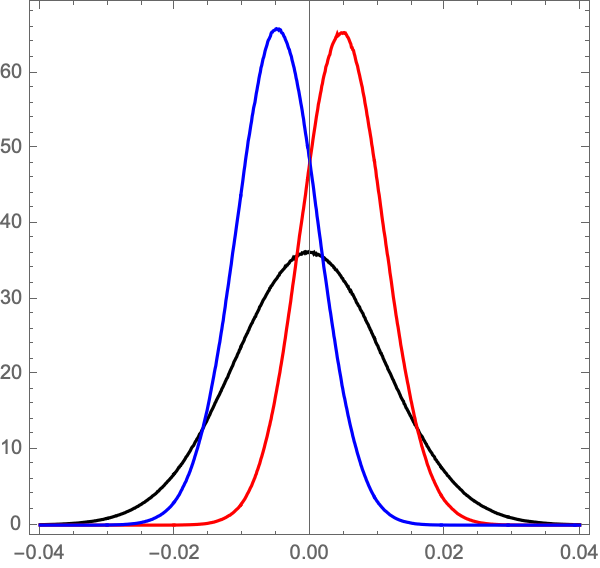
\includegraphics[width=\textwidth]{eigen_dens}
\end{subfigure}~
\begin{subfigure}[b]{0.45\textwidth}
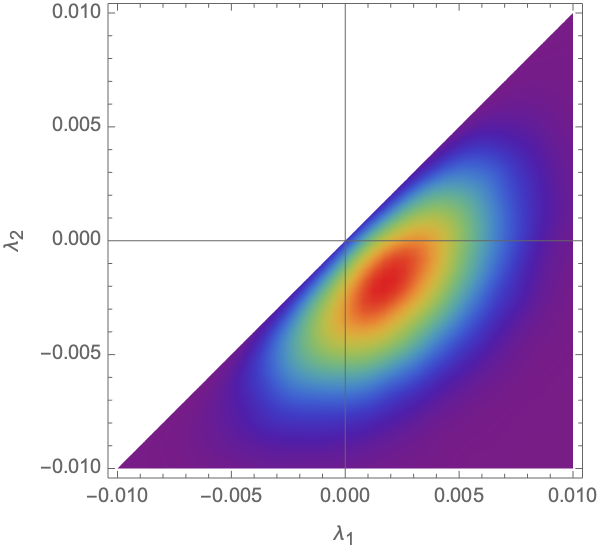
\includegraphics[width=\textwidth]{joint_eigen}
\end{subfigure}
\caption{The distirubtion of the eigenvalue fields. \textit{Left:} the PDF of the initial density perturbation $\delta$ (black) and the initial eigenvalue fields $\mu_{i,t}$ (red and blue). \textit{Right:} the joint distribution of the eigenvalue fields.}\label{fig:eigen_stats}
\end{figure}


%%%%%%%%%%%%%%%%%%%%%%%%%%%%%%%%%%%%%%%%%%%%%%%%%%%%%%%%%%%%%%%%
\section{Constrained random field theory}\label{sec:GRF}
One of the most startling realizations in modern cosmology is that the intricate cosmic web, observed in several cosmological redshift surveys, originated from extremely simple initial conditions. At the moment of recombination, when the baryons and electrons form neutral elements and decouple from the photons, the energy density in our universe, was extremely homogeneous with only tiny density fluctuations. The imprints of these fluctuations have over the last decades been measured with increasing accuracy in the temperature maps of the Cosmic Microwave Background field (CMB) \cite{WMAP:2003, Planck:2016}. Several contemporary paradigms for the big bang, such as inflation theory, envisage these fluctuations to have a quantum origin and interpret them as a realization of a Gaussian random field with only small non-Gaussian deviations. This is in accordance with the most recent statistical analyses of the CMB \cite {Creminelli:2006, Planck:2020} and forms the underpinning of the study of the cosmic web. In this section, we will give a concise definition of Gaussian random field theory. We discuss the implementation of linear constraint Gaussian random field theory, following the notation presented in \cite{Weygaert:1996}, and extend these conditions to non-linear constraints. This will allow us to efficiently implement the caustic conditions and study the properties of the emerging structures.

%%%%%%%%%%%%%%%%%%%%%%%%%%%%%%%%%%%%%%%%%%%%%%%%%%%%%%%%%%%%%%%%
\subsection{Gaussian random fields}
A two-dimensional Gaussian random field $f:\mathbb{R}^2\to \mathbb{R}$ is a generalization of a multi-dimensional normal distribution to the continuum, defined by the probability density
\begin{align}
p(f) = \mathcal{N} e^{- S[f]}\,, \label{eq:functional_Distribution}
\end{align}
with the normalization constant $\mathcal{N}$ and the `action' (in analogy with the Euclidean path integral \cite{Feynman:1965})
\begin{align}
S[f]\equiv \frac{1}{2} \iint [f(\bm{q}_1) - \bar{f}(\bm{q}_1)] K(\bm{q}_1,\bm{q}_2) [f(\bm{q}_2) -\bar{f}(\bm{q}_2)]\mathrm{d}\bm{q}_1 \mathrm{d}\bm{q}_2,\label{eq:action}
\end{align}
defined in terms of the mean field $\bar{f}(\bm{q})$ and the kernel $K(\bm{q}_1,\bm{q}_2)$ \cite{Longuet-Higgins:1957, Adler:1981, bbks:1986}. The probability that the random field $f$ is included in a set of functions $\mathcal{S}$ is defined by the path integral
\begin{align}
P[f \in \mathcal{S}] = \mathcal{N} \int \bm{1}_\mathcal{S}(f) e^{-S[f]}\,\mathcal{D}f\,,
\end{align}
with $\bm{1}_\mathcal{S}$ the identity function\footnote{Defined by $\bm{1}_\mathcal{S}(x)=1$ when $x \in \mathcal{S}$ and $\bm{1}_\mathcal{S}(x)=0$ when $x \notin \mathcal{S}$.} and $\mathcal{D}f$ the path integral measure. The expectation value of a functional $Q[f]$ is given by
\begin{align}
\left\langle Q[f] \right\rangle = \mathcal{N}\int Q[f]\, e^{-S[f]}\,\mathcal{D}f\,,
\end{align}
analogous to the Euclidean path integrals in statistical field theory. It can be shown that the expectation value of the Gaussian random field is given by the mean field
\begin{align}
\langle f(\bm{q})\rangle &= \bar{f}(\bm{q})\,,
\end{align}
and that the two-point correlation function
\begin{align}
\xi(\bm{q}_1, \bm{q}_2) &= \langle (f(\bm{q}_1) - \bar{f}(\bm{q}_1)) (f(\bm{q}_2) - \bar{f}(\bm{q}_2))\rangle\nonumber\\
&= \int (f(\bm{q}_1) - \bar{f}(\bm{q}_1)) (f(\bm{q}_2) - \bar{f}(\bm{q}_2)) e^{-S[f]}\mathcal{D}f
\end{align}
is the inverse of the kernel $K$, \textit{i.e.,}
\begin{align}
\int K(\bm{q}_1,\bm{q}) \xi(\bm{q},\bm{q}_2) \mathrm{d}\bm{q}= \delta_D^{(2)}(\bm{q}_1-\bm{q}_2)\,,\label{eq:defK}
\end{align}
with the two-dimensional Dirac delta function $\delta_D^{(2)}$. The Gaussian random field is thus fully determined by the mean field $\bar{f}$ and the two-point correlation function $\xi$. 

In cosmology, the cosmological principle often leads to the study of statistically homogeneous and isotropic random fields for which the mean field is constant $\bar{f}(\bm{q})=\bar{f}=0$ and the two-point correlation function only depends on the magnitude of the difference of the inserted points, \textit{i.e.}, $\xi(\bm{q}_1,\bm{q}_2)=\xi(\|\bm{q}_1-\bm{q}_2\|)$, and consequently $K(\bm{q}_1,\bm{q}_2)=K(\|\bm{q}_1-\bm{q}_2\|)$. In the present paper, we work with statistically homogeneous and isotropic Gaussian random fields. However, the theory generalizes to generic Gaussian random fields.

The statistical properties of homogeneous and isotropic random fields are most transparently expressed in terms of the Fourier transform of the random field
\begin{align}
\hat{f}(\bm{k}) = \int f(\bm{q})e^{i\bm{k}\cdot \bm{q}}\mathrm{d}\bm{q}\,,
\end{align}
and the inverse transform
\begin{align}
f(\bm{q}) = \int \hat{f}(\bm{k})e^{-i \bm{k} \cdot \bm{q}}\frac{\mathrm{d}\bm{k}}{(2\pi)^2}\,.
\end{align}
The Fourier modes of real-valued Gaussian random fields satisfy the reality condition $\hat{f}(\bm{k}) = \hat{f}^*(-\bm{k})$. Using the double convolution theorem, we express the action \eqref{eq:action} as
\begin{align}
S[f] = \frac{1}{2} \int |\hat{f}(\bm{k})|^2 \hat{K}(\bm{k}) \frac{\mathrm{d}\bm{k}}{(2\pi)^2}\,.
\end{align}
In Fourier space, equation \eqref{eq:defK} takes the form
\begin{align}
\int \hat{K}(\bm{k})\, P(\bm{k})\, e^{i\bm{k}(\bm{q}_1-\bm{q}_2)} \frac{\mathrm{d}\bm{k}}{(2\pi)^2} = \delta_D^{(2)}(\bm{q}_1 - \bm{q}_2)\,,
\end{align}
with the power spectrum defined as the Fourier transform of the two-point correclation function,
\begin{align}
P(\bm{k}) = \int \xi(\bm{q}) \, e^{i\bm{k}\cdot \bm{q}}\mathrm{d}\bm{q}\,,
\end{align}
implying the relation $\hat{K}(\bm{k}) = 1/P(\bm{k})$. For a statistically homogeneous and isotropic random field $P(\bm{k})=P(\|\bm{k}\|)$. The resulting probability density of the Fourier modes is diagonal
\begin{align}
p(\hat{f}) \propto \exp\left[ -\frac{1}{2} \int \frac{|\hat{f}(\bm{k})|^2}{P(\bm{k})} \frac{\mathrm{d}\bm{k}}{(2\pi)^2}\right]\,,
\end{align}
implying the covariance
\begin{align}
\langle \hat{f}(\bm{k}_1)\hat{f}^*(\bm{k}_2) \rangle = (2\pi)^2 \delta_D^{(2)}(\bm{k}_1-\bm{k}_2) P(\bm{k}_1)\,.
\end{align}

% \begin{framed}
% In this paper, we for simplicity always assume the initial gravitational potential to be a realization of a homogeneous and isotropic Gaussian random field with a power-law power spectrum $P(k) \propto k^{n_s}$ smoothed with a Gaussian filter $W(k)=e^{-R_s^2 k^2/2}$ with the spectral index $n_s$ and the smoothing scale $R_s$. The effective power spectrum takes the form 
% \begin{align}
% P_{eff}(k)\propto k^{ns}e^{-R_s^2 k^2}\,.
% \end{align}
% Unless otherwise specified, we use a spectral index $n_s=-1$ and a smoothing length scale $R_s = 5\text{ Mpc}$. 
% \end{framed}


In practice, we often consider realizations of Gaussian random fields on a lattice, or more generally a finite set of linear statistics $\bm{Y}=(Y_1,Y_2,\dots,Y_M)$. In this setting, the functional distribution \eqref{eq:functional_Distribution} reduces to the multi-dimensional Gaussian distribution,
\begin{align}
p(\bm{Y}) = \frac{\exp\left[-\frac{1}{2}  \Delta \bm{Y}^T M^{-1} \Delta \bm{Y}\right]}{[(2\pi)^n \det M]^{1/2}}\,,
\end{align}
with the deviation from the mean $\Delta \bm{Y} = \bm{Y} - \langle \bm{Y}\rangle$ and the covariance matrix
\begin{align}
M = \text{cov}(\bm{Y},\bm{Y}) = \langle \Delta \bm{Y}^T \Delta \bm{Y}\rangle\,.
\end{align}
The distribution of the discrete Fourier modes $\bm{Y}=(\hat{f}(\bm{k}_1),\hat{f}(\bm{k}_2),\dots)$ takes the form 
\begin{align}
p\left(\hat{f}(\bm{k}_1), \hat{f}(\bm{k}_2), \dots\right) = \prod_{i} \frac{1}{\sqrt{2\pi P( \bm{k}_i)}} \exp\left[-\frac{|\hat{f}(\bm{k}_i)|^2}{2P(\bm{k}_i)}\right],
\end{align}
yielding an efficient method to generate realizations (see appendix \ref{ap:GRF}).

The statistical properties of random fields are often conveniently expressed in terms of the moments
\begin{align}
\sigma_i^2 &= \frac{1}{(2\pi)^2} \int \|\bm{k}\|^{2i}P(\bm{k})\mathrm{d}\bm{k}\nonumber\\
&= \frac{1}{2\pi} \int_0^\infty k^{2i+1}P(k)\mathrm{d}k\,,
\end{align}
with the magnitude $k = \|\bm{k}\|$. The power spectrum determines the covariance matrix $M$ through these moments. Whereas the variance of the random field is given by the moment $\sigma_0^2$, \textit{i.e.},
\begin{align}
\langle f(\bm{q})^2 \rangle &= \iint e^{i (\bm{p} - \bm{k})\cdot \bm{q}} \langle \hat{f}(\bm{k})\hat{f}^*(\bm{p})\rangle \frac{\mathrm{d}\bm{k}\mathrm{d}\bm{p}}{(2\pi)^4}\nonumber\\
&=\frac{1}{(2\pi)^2}\int P(\bm{k})\mathrm{d}\bm{k}=\sigma_0^2\,,
\end{align}
the expectation value of the square of the norm of the gradient takes the form
\begin{align}
\langle \|\nabla f(\bm{q})\|^2\rangle &= \langle \partial_1f(\bm{q})^2 + \partial_2 f(\bm{q})^2 \rangle \nonumber \\
&= \iint [(ik_1)(-ip_1)+(ik_2)(-ip_2)] e^{i (\bm{p} - \bm{k})\cdot \bm{q}} \langle \hat{f}(\bm{k})\hat{f}^*(\bm{p})\rangle \frac{\mathrm{d}\bm{k}\mathrm{d}\bm{p}}{(2\pi)^4}\nonumber \\
&=\frac{1}{(2\pi)^2}\int \|\bm{k}\|^2 P(\bm{k})\mathrm{d}\bm{k}=\sigma_1^2\,,
\end{align}
with $\bm{k}=(k_1,k_2)$ and $\bm{p}=(p_1,p_2)$. By statistical isotropy, we obtain the variance of the first-order partial derivatives
\begin{align}
\langle \partial_1 f(\bm{q})^2\rangle =\langle \partial_2 f(\bm{q})^2\rangle =\frac{\sigma_1^2}{2}\,.
\end{align}


%%%%%%%%%%%%%%%%%%%%%%%%%%%%%%%%%%%%%%%%%%%%%%%%%%%%%%%%%%%%%%%%
\subsection{Linear constraints: Gaussian fields}
In this paper, we study how the different geometric features of the cosmic web emerge from different initial conditions. To systematically study these initial conditions we use constrained Gaussian random field theory \cite{Bertschinger:1987, Hoffman:1991, Sheth:1995, Weygaert:1996}. In this section, we develop the theory of linear constraints following the analysis of \cite{Weygaert:1996}. In the next section, we generalize this theory to a large class of non-linear constraints. %We restrict both discussions to statistically homogeneous and isotropic fields with vanishing mean.

For a random field $f$, consider a set of linear constraints
\begin{align}
\Gamma =\{ C_i[f;\bm{q}_i] = c_i,\,\ i=1,\dots,M \}\,,
\end{align}
with the linear functional $C_i[f;\bm{q}]$ assuming the value $c_i$ in $\bm{q}_i$. A linear functional can take the form of the function value at a point
\begin{align}
C[f;\bm{q}'] &= f(\bm{q}')\,,
\end{align}
its derivative at a point
\begin{align}
C[f;\bm{q}'] &= \frac{\partial}{\partial q_i}f(\bm{q}')\,,
\end{align}
or more generally a convolution
\begin{align}
C[f;\bm{q}'] &= \int g(\bm{q}' - \bm{q})f(\bm{q})\mathrm{d}\bm{q}\,,
\end{align}
with the convolution kernel $g$. 

The constraint random field follows the infinite-dimensional distribution
\begin{align}
p(f|\Gamma) = \frac{p(f,\Gamma)}{p(\Gamma)}\,,
\end{align}
where the constraints follow the finite-dimensional Gaussian marginal distribution
\begin{align}
p(\Gamma) = \frac{\exp\left[-\frac{1}{2} \Delta\bm{C}^T Q^{-1} \Delta\bm{C} \right]}{[(2\pi)^M \det Q]^{1/2}}\,,
\end{align}
with the vector $\bm{C}=(C_1[f;\bm{q}_1], \dots, C_M[f;\bm{q}_M])$ and the covariance matrix $Q = \text{cov}(\bm{C}, \bm{C})$. We can write the constraint distribution as the Gaussian probability density
\begin{align}
p(f|\Gamma) \propto  \exp\left[-\frac{1}{2} \left[\iint f(\bm{q}_1) K(\|\bm{q}_1 - \bm{q}_2\|) f(\bm{q}_2)\mathrm{d}\bm{q}_1 \mathrm{d}\bm{q}_2 -\Delta \bm{C}^TQ^{-1}\Delta \bm{C}\right]\right],\label{eq:constraint1}
\end{align}
in the space of functions satisfying the constraints $\Gamma$. In appendix \ref{ap:constraintDensity}, we derive the mean field
\begin{align}
\bar{f}_{\bm{c}}(\bm{q})&=\langle f(\bm{q})|\Gamma\rangle \nonumber \\
&= \bar{f}(\bm{q}) + \sum_{i,j=1}^M\xi_i (\bm{q})\xi_{ij}^{-1}(c_j-\bar{C}_j)\,,
\end{align}
and the covariance
\begin{align}
\text{cov}(f(\bm{q}_1),f(\bm{q}_2)|\Gamma)  = \xi(\bm{q}_1,\bm{q}_2) - \sum_{i,j=1}^M\xi_i(\bm{q}_1)\xi_{ij}^{-1}\xi_j(\bm{q}_2)\,,
\end{align}
with the covariance of the random field and the constraints $\xi_{i}(\bm{q}) = \text{cov}( f(\bm{q}), C_i)$ and the covariance matrix of the constraints $\xi_{ij} = \text{cov}( C_i ,C_j)$. Remarkably, the covariance $\text{cov}(f(\bm{q}_1),f(\bm{q}_2)|\Gamma)$ is independent of the value $\bm{c}$ the constraint $\bm{C}$ assumes. This is a special property of Gaussian distributions and linear constraints. Moreover, the residue with respect to the mean field is normally distributed (see appendix \ref{ap:constraintDensity}). Consequently, the probability density takes the form
\begin{align}
p( f|\Gamma) \propto  \exp\left[-\frac{1}{2} \iint \delta{f}(\bm{q}_1) \tilde{K}(\bm{q}_1,\bm{q}_2) \delta f(\bm{q}_2)\mathrm{d}\bm{q}_1 \mathrm{d}\bm{q}_2 \right]\,,\label{eq:constraint2}
\end{align}
with the residue $\delta f = f-\langle f(\bm{q})|\Gamma\rangle$ and the constrained kernel $\tilde{K}$ defined as the inverse of the constrained two-point correlation function, \textit{i.e.},
\begin{align}
\int \tilde{K}(\bm{q}_1,\bm{q}) \left[\xi(\bm{q},\bm{q}_2) - \sum_{i,j=1}^M\xi_i(\bm{q})\xi_{ij}^{-1}\xi_j(\bm{q}_2)\right]\mathrm{d}\bm{q}= \delta_D^{(2)}(\bm{q}_1-\bm{q}_2)\,.
\end{align}
Note that earlier papers \cite{Bertschinger:1987, Hoffman:1991, Sheth:1995, Weygaert:1996} worked in the space of functions satisfying the constraints $\Gamma$, neglecting the correction $\sum_{i,j=1}^M\xi_i(\bm{q})\xi_{ij}^{-1}\xi_j(\bm{q}_2)$, and using the original kernel $K$ for the residue. In this study, we prefer to work in the space of unrestricted functions, as the correction makes the inhomogeneity and anisotropy of the residue manifest. These properties are most clearly observed in the variance of the residue,
\begin{align}
\langle \delta f(\bm{q})^2|\Gamma \rangle = \sigma_0^2- \sum_{i,j=1}^M\xi_i(\bm{q})\xi_{ij}^{-1}\xi_j(\bm{q})\,,\label{eq:variance_Linear}
\end{align}
which vanishes on the constraints. Away from the constraints, the variance of the residue approaches the variance of the unconstrained field $\text{var}(f)=\sigma_0^2$. Note that this relation implies an analogous relation for the Laplacian of the random field $\nabla^2 f$, \textit{i.e.}, we find the mean
\begin{align}
\langle \nabla^2 f(\bm{q})\,|\,\Gamma\rangle = \nabla^2 f_{\bm{c}}(\bm{q})
\end{align}
and the variance
\begin{align}
\langle \delta (\nabla^2f(\bm{q}_1))^2\,|\,\Gamma \rangle = \sigma_2^2- \sum_{i,j=1}^M\nabla^2\xi_i(\bm{q})\xi_{ij}^{-1}\nabla^2\xi_j(\bm{q})\,.\label{eq:variance_Linear_Laplace}
\end{align}


The Hoffman-Ribak method cleverly uses the property that the statistics of the residue $\delta f$ are independent of $\bm{c}$, to generate realizations of the constraint Gaussian random field \cite{Hoffman:1991, Weygaert:1996}. Firstly, generate a realization $g$ of the unconstraint Gaussian random field with the required power spectrum. Secondly, evaluate the constraints for this realization $C_i[g;\bm{q}'_i]=d_i$ and the corresponding mean field $\bar{g}$. The statistical properties of the residue with respect to this mean field $\delta g = g-\bar{g}$ are independent of the value the constraints assume and thus identical to the properties of the residue $\delta f$. We can thus identify the residue $\delta g$ of the field $g$ with the residue $\delta f$ of the constrained field $f$. By adding the residue of the unconstraint field to the mean field with the required constraints, we obtain the realization of the constrained Gaussian random field. For more details see appendix \ref{ap:GRF}.

To judge the relevance of a particular set of constraints, it is useful to evaluate the $\chi^2$ of the set of values $c_i$,
\begin{align}
\chi^2 = \sum_{i,j=1}^M (c_i-\bar{C}_i)\, \xi_{ij}^{-1}(c_j-\bar{C}_j)\,,
\end{align}
which follows the chi-squared distribution with $M$ degrees of freedom. This is the Mahalanobis distance. The probability that one obtains a $\chi^2$ higher than this value in an unconstrained Gaussian random field, with the same power spectrum, is given by $\Gamma\left(\frac{M}{2}, \frac{\chi^2}{2}\right)/\Gamma\left(\frac{M}{2}\right)$, with the gamma function $\Gamma(x)$ and the upper incomoplete gamma function $\Gamma(s,x)$.

%%%%%%%%%%%%%%%%%%%%%%%%%%%%%%%%%%%%%%%%%%%%%%%%%%%%%%%%%%%%%%%%
\subsection{Non-linear constraints: formalism}
For the systematic investigation of the caustic skeleton, we extend constraint Gaussian random field theory to include non-linear constraints. More specifically, we extend the theory of linear constraints to the large class of non-linear constraints expressed in terms of a finite number of linear statistics.

Consider the set of linear functionals $C_i[f,\bm{q}_i]$ with $i=1,\dots,M$ and the space of values $\bm{c}=(c_1,\dots,c_M)$ the linear functionals can assume $\mathbb{R}^M$. On this space, we define a set of functions $\mathcal{C}_i:\mathbb{R}^M \to \mathbb{R}$ with $i=1,\dots,N$ and $N\leq M$, and the non-linear constraint $\Gamma = \{\mathcal{C}_i(\bm{C}) = 0\}_{i=1}^N$. We can visualize this geometrically by considering the $(M-N)$-dimensional constraint manifold $\mathcal{M}_\mathcal{C}$ in the space of the $M$ linear constraints
\begin{align}
\mathcal{M}_{\mathcal{C}} = 
\{\bm{c}\, |\, \mathcal{C}_i(\bm{c}) = 0 \text{ for all } i=1,\dots,N\}.
\end{align}
See figure \ref{fig:constraintManifold} for a sketch of this constraint manifold. On the manifold $\mathcal{M}_\mathcal{C}$, the constraint probability density is proportional to the original Gaussian distribution
\begin{framed}
\begin{align}
p(\bm{c}\,|\,\bm{c}\in \mathcal{M}_{\mathcal{C}})  = \frac{p(\bm{c})}{\int_{\mathcal{M}_\mathcal{C}} p(\bm{c})\, \mathrm{d}\bm{c}}\,.
\end{align}
\end{framed}
Note that the curvature of $\mathcal{M}_\mathcal{C}$ generally makes the induced density $p(\bm{c}\,|\,\bm{c}\in \mathcal{M}_{\mathcal{C}})$ non-Gaussian. We extend constraint Gaussian random field theory to include non-linear constraints by studying the finite-dimensional probability density $p(\bm{c}\,|\,\bm{c}\in \mathcal{M}_{\mathcal{C}})$:



\begin{figure}
\centering
\begin{subfigure}[b]{0.49\textwidth}
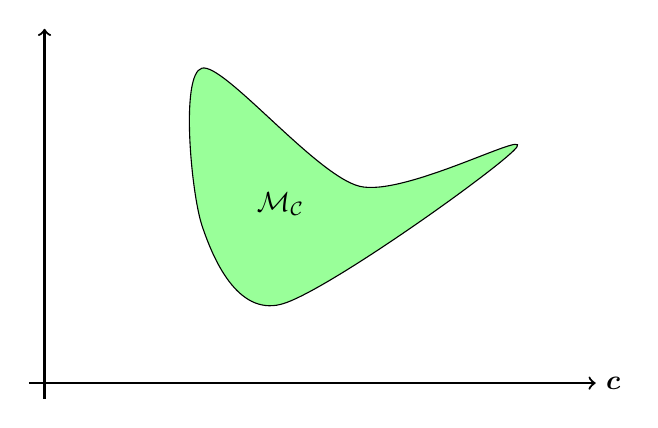
\begin{tikzpicture}
%\draw[draw=black] (0,0) rectangle ++(7,5);
\draw[->, thick] (-0.2,0)--(7,0) node[right]{$\bm{c}$};
\draw[->, thick] (0,-0.2)--(0,4.5);
%\draw [fill=blue!80] plot [mark=none, smooth cycle] coordinates {(2,2) (3,1) (6,3) (4,2.5) (2,4)};
\draw [fill=green!40] plot [mark=none, smooth cycle] coordinates {(2,2) (3,1) (6,3) (4,2.5) (2,4)};
%\draw [fill=lime!70] plot [mark=none, smooth cycle] coordinates {(2,2) (3,1) (6,3) (4,2.5) (2,4)};
\node[above] at (3,2) {$\mathcal{M}_\mathcal{C}$};
\end{tikzpicture}
\end{subfigure}
\caption{The constraint manifold $\mathcal{M}_\mathcal{C}$ in the space of linear constraint values.}\label{fig:constraintManifold}
\end{figure}


\begin{itemize}
\item
The problem of generating realizations of the more general constraints fields is reduced to sampling realizations of the distribution $p(\bm{c}|\bm{c}\in \mathcal{M}_\mathcal{C})$. Given a sample $\bm{c}$, we use the Hoffman-Ribak method to generate the realization.


\begin{framed}
\item
The mean field of the constrained field assumes the surprisingly suggestive form 
\begin{align}
\bar{f}_{\mathcal{C}}(\bm{q}) =\bar{f}_{\bar{\bm{c}}}(\bm{q})\,,
\end{align}
with the mean constraint
\begin{align}
\bar{\bm{c}} &\equiv \langle \bm{c} \,|\, \Gamma\rangle = \int_{\bm{c} \in \mathcal{M}_{\mathcal{C}}}  \bm{c}\, p(\bm{c}\,|\,\bm{c}\in \mathcal{M}_{\mathcal{C}}) \mathrm{d}\bm{c}\,,
\end{align}
\end{framed}
following from the realization  
\begin{align}
\bar{f}_{\mathcal{C}}(\bm{q}) 
&=\left\langle f(\bm{q})\,|\,\Gamma\right \rangle \nonumber\\
&= \int_{\bm{c} \in \mathcal{M}_{\mathcal{C}}} \bar{f}_{\bm{c}}(\bm{q})\, p(\bm{c}|\bm{c}\in \mathcal{M}_{\mathcal{C}}) \mathrm{d}\bm{c}\nonumber\\
&= \sum_{i,j=1}^M\xi_i(\bm{q}) \xi_{ij}^{-1}\int_{\bm{c} \in \mathcal{M}_{\mathcal{C}}}  (c_j-\bar{C}_j)\, p(\bm{c}\,|\,\bm{c}\in \mathcal{M}_{\mathcal{C}}) \mathrm{d}\bm{c}\nonumber\\
&= \sum_{i,j=1}^M \xi_i(\bm{q}) \xi_{ij}^{-1} (\bar{c}_j-\bar{C}_j)\nonumber\\
&= \bar{f}_{\bar{\bm{c}}}(\bm{q})\,.
\end{align}

\begin{framed}
\item
The residue $\delta f = f - \bar{f}_{\mathcal{C}}$ is generically no longer a Gaussian random field. The variance of the residue yields
\begin{align}
\left \langle \delta f (\bm{q})^2\,|\,\Gamma\right\rangle =
\sigma_0^2 - \sum_{i,j=1}^M\xi_i(\bm{q}) \zeta_{ij}^{-1} \xi_j(\bm{q}) 
\,,\label{eq:variance_Nonlinear}
\end{align}
with the coefficients
\begin{align}
\zeta_{ij}^{-1}= \xi_{ij}^{-1}-\sum_{k,l=1}^M\xi_{ik}^{-1}\text{cov}(c_k, c_l\,|\,\bm{c}\in\mathcal{M}_\mathcal{C})\xi_{lj}^{-1}\,,
\end{align}
\end{framed}
where $\text{cov}(c_j, c_l\,|\,\bm{c}\in\mathcal{M}_\mathcal{C})$ captures the geometry of the constraint manifold $\mathcal{M}_\mathcal{C}$, following directly from
\begin{align}
\left \langle \delta f (\bm{q})^2\,|\,\Gamma\right\rangle 
&= \int_{\mathcal{M}_\mathcal{C}} \langle (f(\bm{q})-\bar{f}_{\bar{\bm{c}}}(\bm{q}))^2\,|\,C_i[f,\bm{q}_i]=c_i\rangle p(\bm{c}\,|\,\bm{c}\in\mathcal{M}_{\mathcal{C}})\mathrm{d}\bm{c}\nonumber \\
&= \int_{\mathcal{M}_\mathcal{C}} \langle f^2(\bm{q})\,|\,C_i[f,\bm{q}_i]=c_i\rangle p(\bm{c}\,|\,\bm{c}\in\mathcal{M}_{\mathcal{C}})\mathrm{d}\bm{c} - \bar{f}_{\bar{\bm{c}}}^2(\bm{q})\nonumber \\
&= \int_{\mathcal{M}_\mathcal{C}} \langle (f(\bm{q})-\bar{f}_{\bm{c}}(\bm{q}))^2\,|\,C_i[f,\bm{q}_i]=c_i\rangle p(\bm{c}\,|\,\bm{c}\in\mathcal{M}_{\mathcal{C}})\mathrm{d}\bm{c} \nonumber \\
&\ \ +\int_{\mathcal{M}_\mathcal{C}} (\bar{f}_{\bm{c}}(\bm{q})- \bar{f}_{\bar{\bm{c}}}(\bm{q}))^2p(\bm{c}\,|\,\bm{c}\in\mathcal{M}_{\mathcal{C}})\mathrm{d}\bm{c} \nonumber \\
&=  \sigma_0^2 - \sum_{i,j=1}^M\xi_i(\bm{q}) \xi_{ij}^{-1} \xi_j(\bm{q}) + \sum_{i,j,k,l=1}^M \xi_{i}(\bm{q})\xi_{ij}^{-1}\text{cov}(c_j, c_l\,|\,\bm{c}\in\mathcal{M}_\mathcal{C})\xi_{lk}^{-1}\xi_{k}(\bm{q})\nonumber\\
&=
\sigma_0^2 - \sum_{i,j=1}^M\xi_i(\bm{q}) \zeta_{ij}^{-1} \xi_j(\bm{q})\,,
\end{align}
where
\begin{align}
\int_{\mathcal{M}_\mathcal{C}} (\bar{f}_{\bm{c}}(\bm{q})- \bar{f}_{\bar{\bm{c}}}(\bm{q}))^2p(\bm{c}\,|\,\bm{c}\in\mathcal{M}_{\mathcal{C}})\mathrm{d}\bm{c} 
&= \text{var}\left(\sum_{i,j=1}^M\xi_i(\bm{q})\xi_{ij}^{-1}c_j\,|\,\bm{c}\in \mathcal{M}_\mathcal{C}\right)\\
&=\sum_{i,j,k,l=1}^M \xi_i(\bm{q})\xi_{ij}^{-1}\text{cov}(c_j,c_k\,|\,\bm{c}\in\mathcal{M}_\mathcal{C})\xi_{kl}^{-1}\xi_l(\bm{q})\,.\nonumber
\end{align}
Note that the variance of the residue with respect to the non-linear constraint is no longer independent of the values the constraint assumes. When $\mathcal{M}_\mathcal{C}$ consists of a point, we recover the linear formula.
\end{itemize}

A similar relation applies to the Laplacian of the random field, which in our context represents the density perturbations. Following an analogous derivation, we obtain the mean
\begin{align}
\langle \nabla^2 f(\bm{q})\,|\,\Gamma\rangle = \sum_{i,j=1}^M \nabla^2\xi_i(\bm{q})\xi_{ij}^{-1}(\bar{c}_j-\bar{C}_j)
\end{align}
and the variance
\begin{align}
\langle \delta (\nabla^2 f(\bm{q}))\,|\,\Gamma\rangle = \sigma_2^2 - \sum_{i,j=1}^M \nabla^2 \xi_i(\bm{q})\zeta_{ij}^{-1}\nabla^2\xi_j(\bm{q})\,,
\end{align}
with the same $\bar{\bm{c}}$ and $\zeta_{ij}$.



%%%%%%%%%%%%%%%%%%%%%%%%%%%%%%%%%%%%%%%%%%%%%%%%%%%%%%%%%%%%%%%%
\subsection{Non-linear constraints: case study}
A good example of a non-linear constraint is the requirement that the gradient of the Gaussian random field has a unit norm $\|\nabla f(\bm{q}_c)\|=1$. For this condition, we consider the space of first-order derivatives
\begin{align}
\bm{C}=(\partial_x f, \partial_y f)\,,
\end{align}
and the non-linear constraint 
\begin{align}
\mathcal{C}(\bm{C})=\partial_x f^2 +  \partial_y f^2 - 1=0\,.
\end{align}
The constraint manifold $\mathcal{M}_\mathcal{C}=\{(\partial_xf,\partial_yf)\, |\, \partial_xf^2+\partial_yf^2=1\}$ is the unit circle in the space of first order derivatives (see figure \ref{fig:constraintManifold_example}).

For a statistically isotropic Gaussian random field, the constrained probability density is uniform $p(\bm{c}\, |\, \bm{c}\in\mathcal{M}_\mathcal{C}) = 1/(2\pi)$. After sampling from the constraint manifold, we construct a corresponding realization using linear constrained Gaussian random field theory. Both the mean and the covariance of the constraint value with respect to the constraint manifold vanish.

When the Gaussian random field is not statistically isotropic, the constraint density $p(\bm{c}\, |\, \bm{c}\in\mathcal{M}_\mathcal{C})$ is no longer uniformly distributed. We can construct realizations of the constrained Gaussian random field using rejection sampling on the constraint manifold. First, determine the maximum $max$ of $p(\bm{c})$ restricted to $\mathcal{M}_\mathcal{C}$. Secondly, generate a uniformly sampled point $\bm{c}$ on the unit circle $\mathcal{M}_\mathcal{C}$. Finally, we accept this sample $\bm{c}$ with probability $p(\bm{c})/max$. Once we have sampled the points on the constraint manifold $\mathcal{M}_\mathcal{C}$, we again construct a corresponding realization using linear constrained Gaussian random field theory. It is also straightforward to sample the mean and covariance of the constraint value $\bm{c}$ on the constraint manifold $\mathcal{M}_\mathcal{C}$.



\begin{figure}
\centering
\begin{subfigure}[b]{0.49\textwidth}
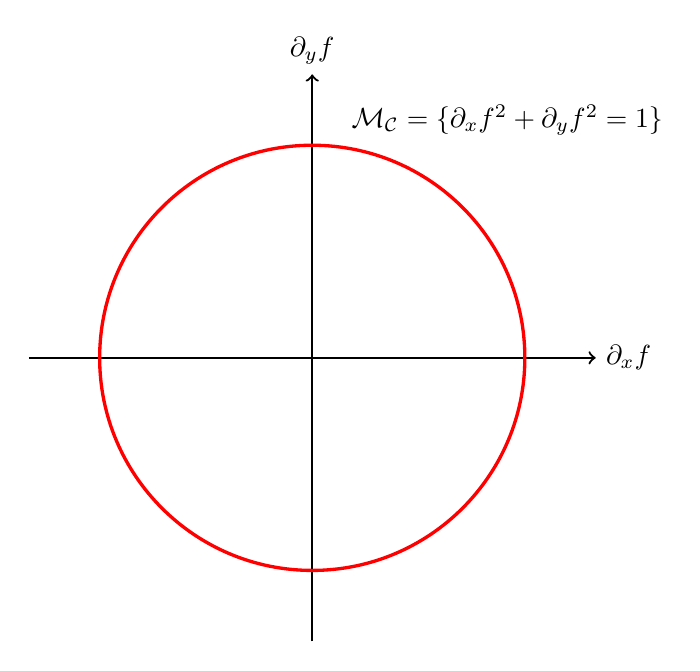
\begin{tikzpicture}[scale=0.9]
%\draw[help lines, color=gray!30, dashed] (-0.9,-0.9) grid (4.9,4.9);
\draw[->, thick] (-4,0)--(4,0) node[right]{$\partial_x f$};
\draw[->, thick] (0,-4)--(0,4) node[above]{$\partial_y f$};
\draw[color=red, very thick](0,0) circle (3);
\node[above] at (2.75,3) {$\mathcal{M}_\mathcal{C}=\{\partial_xf^2+\partial_yf^2=1\}$};
\end{tikzpicture}
\end{subfigure}
\caption{The constraint manifold $\mathcal{M}_\mathcal{C}=\{\partial_xf^2+\partial_yf^2=1\}$ in the space of first order derivatives $(\partial_x f,\partial_yf)$ for the non-linear constraint $\|\nabla f\|=1$.}\label{fig:constraintManifold_example}
\end{figure}



%%%%%%%%%%%%%%%%%%%%%%%%%%%%%%%%%%%%%%%%%%%%%%%%%%%%%%%%%%%%%%%%
\section{Constraint initial conditions of the caustic skeleton}\label{sec:caustic_skeleton_constraints}
Given non-linear constrained Gaussian random field theory and the caustic conditions, we study the progenitors of the filaments and clusters in the Zel'dovich approximation. Given the displacement field 
\begin{align}
\bm{s}_t(\bm{q}) = -b_+(t) \nabla_{\bm{q}} \Psi(\bm{q}),
\end{align}
it is convenient to express the deformation tensor
\begin{align}
\bm{\psi}(\bm{q}) = \begin{pmatrix} T_{11}(\bm{q}) & T_{12}(\bm{q}) \\ T_{12}(\bm{q}) & T_{22}(\bm{q})\end{pmatrix}\,,
\end{align}
in terms of the partial derivatives of the displacement potential $T_{ij\dots k}=\frac{\partial}{\partial q_i}\frac{\partial}{\partial q_j}\dots \frac{\partial}{\partial q_k}\Psi$. Define the eigenvalue and eigenvector fields of $\bm{\psi}$ with the eigenequation
\begin{align}
\bm{\psi}(\bm{q}) \bm{v}_i(\bm{q}) = \lambda_i(\bm{q}) \bm{v}_i(\bm{q}),
\end{align}
with the ordering $\lambda_1\geq \lambda_2$ and normalize the eigenvector field to unity, \textit{i.e.}, $\|\bm{v}_{i}\|=1$. We can express the eigenvalue and eigenvector fields explicitly in terms of the second-order derivatives of the deformation potential
\begin{align}
\lambda_{1,2} &= \frac{1}{2}\left[T_{11}+T_{22} \pm \sqrt{4 T_{12}^2+(T_{11}-T_{22})^2}\right]\,,\\
\bm{v}_{1,2} &\propto  \left(T_{11}-T_{22} \pm \sqrt{4 T_{12}^2+(T_{11}-T_{22})^2}, 2 T_{12}\right)\,,
\end{align}
showing their non-linear dependence on the deformation potential. 
%\begin{framed}
%In the study below, we assume a power-law power spectrum for the gravitational potential
%\begin{align}
%P(k)=k^{n_s} e^{-R_s^2 \|\bm{k}\|^2}
%\end{align}
%with the spectral index $n_s=-1$ and the Gaussian smoothing at the length scale $R_s = 5 \text{ Mpc}$.
%\end{framed}
%%%%%%%%%%%%%%%%%%%%%%%%%%%%%%%%%%%%%%%%%%%%%%%%%%%%%%%%%%%%%%%%
\subsection{Cusp filament}
The cusp caustic forming at time $t$, corresponding to the largest eigenvalue field $\lambda_1$, satisfies the conditions
\begin{align}
b_+(t) \lambda_1(\bm{q}_c) &= 1\,, \\
 \bm{v}_1(\bm{q}_c) \cdot \nabla\lambda_1(\bm{q}_c) &= 0\,.
\end{align}
The orientation of the cusp is determined by the normal vector
\begin{align}
\bm{n} =  \nabla(\bm{v}_1(\bm{q}_c) \cdot \nabla\lambda_1(\bm{q}_c))\,,
\end{align}
which makes an angle 
\begin{align}
\alpha = \text{sign}(\bm{v}_2\cdot \bm{n}) \arccos\left(\frac{|\bm{v}_1\cdot \bm{n}|}{\|\bm{n}\|}\right)
\end{align}
with respect the corresponding eigenvector $\bm{v}_1$. As both the cusp curve and the eigenvector field consist of lines, the angle $\alpha$ assumes a value in the interval $[-\pi/2,\pi/2]$. 

In figure \ref{fig:meanCusp}, we plot the mean field of the cusp filament with the condition that the center of the box has a cusp caustic oriented along the vertical direction. The gravitational potential is close to a dipole. The blue central structure yields an inflow of matter, whereas two red structures around the blue structure yield two outflow regions. The critical curve in the eigenvalue field consists of an elongated oval which forms the traditional Zel'dovich pancake in the Zel'dovich approximation. The cusp curve bisects the oval in Lagrangian space and the pancake Eulerian space.

On average, the orientation of the cusp curve is normal to the eigenvector field $\bm{v}_1$. Figure \ref{fig:alpha} plots the distribution  of the angle $\alpha$. The distribution consists of a bell curve centered at $\alpha =0$ and an exponential fall-off towards the angles $\alpha =\pm \pi/2$.

\begin{figure}
\centering
\begin{subfigure}[b]{0.32\textwidth}
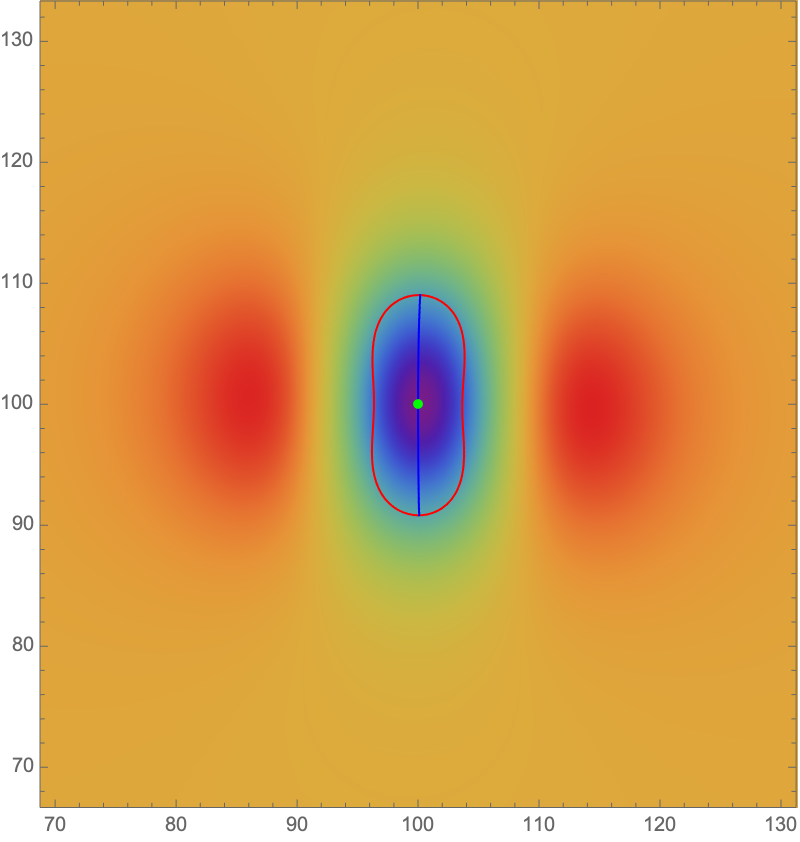
\includegraphics[width=\textwidth]{Cusp_mean_Phi}
\end{subfigure}~
\begin{subfigure}[b]{0.32\textwidth}
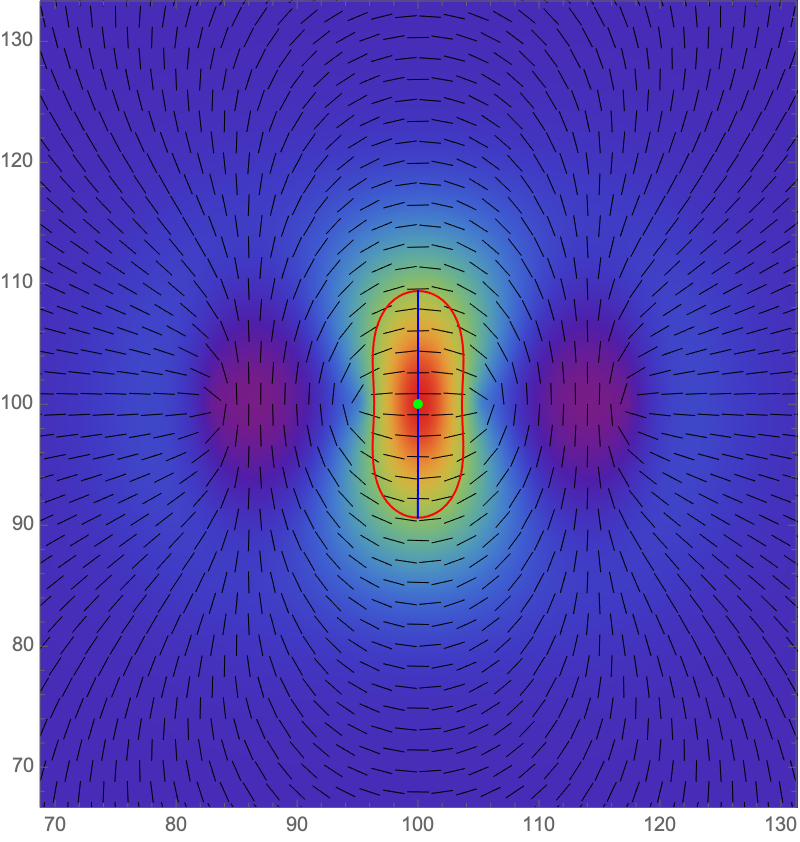
\includegraphics[width=\textwidth]{Cusp_mean_L}
\end{subfigure}~
\begin{subfigure}[b]{0.32\textwidth}
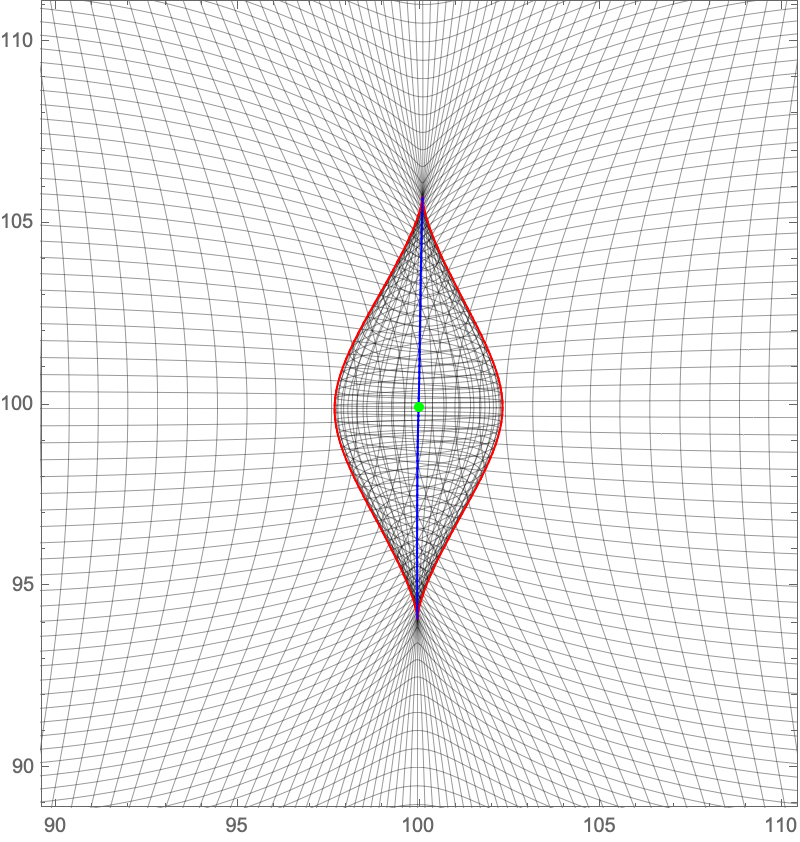
\includegraphics[width=\textwidth]{Cusp_mean_Z}
\end{subfigure}
\caption{The mean cusp caustic. \textit{Left:} the gravitational potential. \textit{Centre:} the first eigenvalue and eigenvector fields. \textit{Right:} The Zel'dovich approximation}\label{fig:meanCusp}
\end{figure}

\begin{figure}
\centering
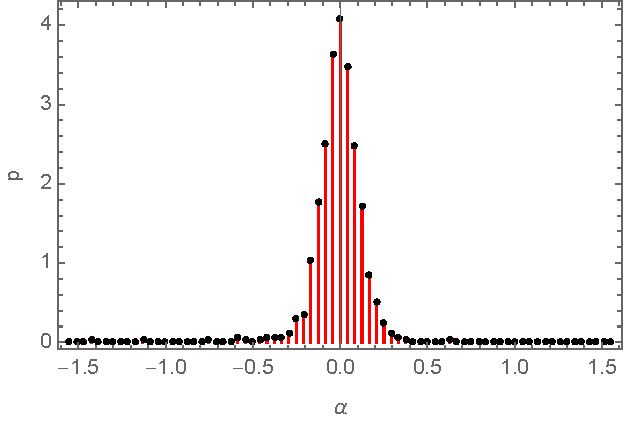
\includegraphics[width=0.5\textwidth]{alpha}
\caption{The distribution of the angle $\alpha$ between the cusp curve and the eigenvector field.} 
\label{fig:alpha}
\end{figure}

%%%%%%%%%%%%%%%%%%%%%%%%%%%%%%%%%%%%%%%%%%%%%%%%%%%%%%%%%%%%%%%%
\subsubsection{Sampling the constraint manifold}
To analyze the constraint field of the cusp caustic, we work in the eigenframe of the deformation tensor for which $\bm{v}_1=(1,0)$ and $\bm{v}_2=(0,1)$. In this frame, the caustic conditions yield a set of linear conditions on the second and third-order derivatives of the deformation potential
\begin{align}
T_{11}=1/b_+(t)\,, \quad T_{12}=0\,,\quad T_{22}\leq T_{11}\,,\quad T_{111}=0\,.\label{eq:cusp_cond_1}
\end{align}
The normal vector yields the non-linear form
\begin{align}
\bm{n}=\left(T_{1111} + \frac{3T_{112}^2}{T_{11}-T_{22}}, T_{1112} + \frac{3T_{112}T_{122}}{T_{11}-T_{22}}\right)\,.\label{eq:cusp_cond_2}
\end{align}
For a derivation of these identities see appendix \ref{ap:eigenvalueRel}.

For simplicity, let's first ignore the orientation of the cusp curve and consider a cusp curve passing through the center of the box, with the relevant linear statistics $Y=(T_{11}$,$T_{12}$,$T_{22}$,$T_{111})$, whose probability density factorizes into the density of the joint distribution of $T_{11}$ and $T_{22}$ and the one-dimensional Gaussian distributions for $T_{12}$ and $T_{111}$, \textit{i.e.},
\begin{align}
p(T_{11},T_{12},T_{22},T_{111}) = p(T_{11},T_{22})p(T_{12})p(T_{111})\,.
\end{align}
Generally, two derivatives of a Gaussian random field at a point are independent if and only if they together consist of an odd number of derivatives in either the $q_1$ or the $q_2$ direction. The conditional probability density takes the form
\begin{align}
p&(T_{11},T_{12},T_{22},T_{111}|,T_{22}\leq T_{11}=1/b_+,T_{12}=0,T_{111}=0) \nonumber\\
&= p(T_{22}| T_{22} \leq T_{11}=1/b_+)\nonumber\\
&= \mathcal{N} e^{-\frac{3(T_{11} + T_{22})^2 - 8 T_{11} T_{22}}{2 \sigma_2^2}}\big|_{T_{11}=1/b_+}\,,
\end{align}
with the normalization constant $\mathcal{N}$. After sampling $T_{22}$ from this distribution, we use linear constrained random field theory to obtain the corresponding realization. Note that this procedure is equivalent to generating realizations for the linear constraints $T_{11}=1/b_+,T_{12}=T_{111}=0$ and rejecting realizations for which $T_{22} > 1/b_+$. Given these realizations, it is straightforward to compute the angle $\alpha$ and sample the distribution (see figure \ref{fig:alpha}).

The orientation of the cusp curve is fully characterized by the derivatives  
\begin{align}
Y=(T_{11},T_{12},T_{22},T_{111},T_{112},T_{122},T_{1111},T_{1112})\,,
\end{align}
with the conditional distribution
\begin{align}
&p(T_{11},T_{12},T_{22},T_{111},T_{112},T_{122},T_{1111},T_{1112}|T_{22} \leq T_{11}=1/b_+, T_{111}=0)\\
&=
p(T_{11},T_{22},T_{1111}|T_{22}\leq T_{11}=1/b_+)p(T_{12}T_{1112}|T_{12}=0)p(T_{111},T_{122}|T_{111}=0)p(T_{112})\,.\nonumber
\end{align}
We can generate realizations for which the cusp curve is vertical in the center of the box, by sampling this distribution with the additional constraint that $\bm{n} \propto (1,0)$. However, for this paper, we will use a slightly different method based on the sampling method described above. Given a realization, we first evaluate all second, third, and fourth-order derivatives and evaluate the angle $\alpha$. Subsequently, rotate these derivatives by an angle $\alpha$ (following appendix \ref{ap:rotations}). The resulting derivatives form a representative sample of a cusp curve running vertically through the center of the box. By generating the linear constraint realizations with these rotates derivatives, we obtain a realization of the Gaussian random field required cusp curve.

%%%%%%%%%%%%%%%%%%%%%%%%%%%%%%%%%%%%%%%%%%%%%%%%%%%%%%%%%%%%%%%%
\subsection{Swallowtail cluster}
The swallowtail caustic forming at time $t$, corresponding to the largest eigenvalue field $\lambda_1$, satisfies the conditions
\begin{align}
b_+(t) \lambda_1(\bm{q}_c) = 1\,,\\
\quad \bm{v}_1(\bm{q}_c) \cdot \nabla\lambda_1(\bm{q}_c) = 0\,,\\
 \quad\bm{v}_1(\bm{q}_c)\cdot \nabla( \bm{v}_1(\bm{q}_c) \cdot \nabla\lambda_1(\bm{q}_c)) = 0\,.
\end{align}
The cusp curve in the swallowtail caustic is parallel to the eigenvector field $\bm{v}_1$ since $\bm{v}_1 \cdot \bm{n}=0$ or equivalently $\alpha = \pm \pi/2$. The swallowtail caustic does not require us to fix its orientation. However, we do need to specify the direction, normal to the fold curve, in which the swallowtail structure forms. We will here use the condition $\bm{v}_2 \cdot \nabla \lambda_1(\bm{q}) <0$.

In figure \ref{fig:meanSwallowtail}, we plot the mean field of the swallowtail cluster. The gravitational potential is again close to a dipole. However, note the development of an asymmetry with respect to the horizontal axis. The blue central structure yields an inflow of matter, whereas two red structures around the blue structure yield two outflow regions. The critical curve in the eigenvalue field consists of an elongated oval with two bifurcations in the upper half-plane. The cusp curves form a trident inside the fold curve. In the Zel'dovich approximation, the caustic skeleton consists of a Zel'dovich pancake with two whiskers in the upper half-plane. 



\begin{figure}
\centering
\begin{subfigure}[b]{0.32\textwidth}
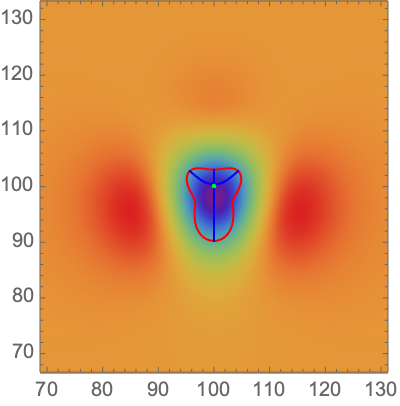
\includegraphics[width=\textwidth]{Swallowtail_mean_Phi}
\end{subfigure}~
\begin{subfigure}[b]{0.32\textwidth}
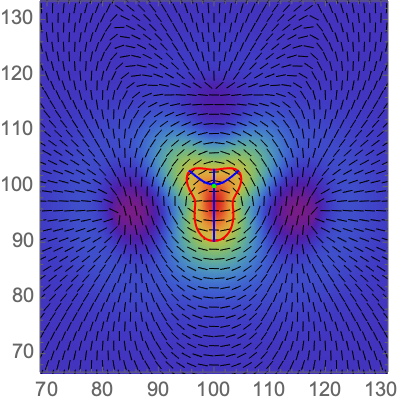
\includegraphics[width=\textwidth]{Swallowtail_mean_L}
\end{subfigure}~
\begin{subfigure}[b]{0.32\textwidth}
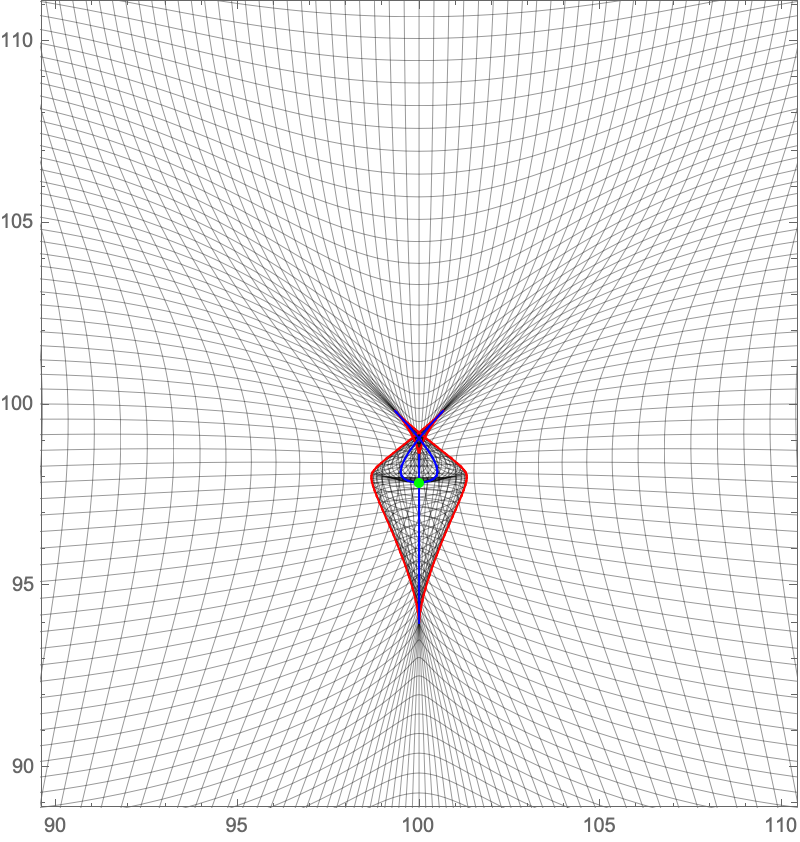
\includegraphics[width=\textwidth]{Swallowtail_mean_Z}
\end{subfigure}
\caption{The mean swallowtail caustic. \text{Left:} the gravitational potential. \textit{Centre:} the first eigenvalue and eigenvector fields. \textit{Right:} The Zel'dovich approximation}\label{fig:meanSwallowtail}
\end{figure}


%%%%%%%%%%%%%%%%%%%%%%%%%%%%%%%%%%%%%%%%%%%%%%%%%%%%%%%%%%%%%%%%
\subsubsection{Sampling the constraint manifold}
In the eigenframe, the caustic conditions for the swallowtail take the form
\begin{align}
T_{11}=1/b_+(t)\,, \quad T_{12}=0\,,\quad T_{22}\leq T_{11}\,,\quad T_{111}=0\,, \quad T_{1111}+\frac{3T_{112}^2}{T_{11}-T_{22}} =0\,.
\end{align}
The condition that specifies the direction in which the swallowtail develops, $\bm{v}_2 \cdot \nabla \lambda_1  <0$, yields the simple form 
\begin{align}
T_{112} <0\,.
\end{align}
See appendix \ref{ap:eigenvalueRel} for a detailed derivation. 

The swallowtail caustic is determined by the linear statistics $Y=(T_{11},$ $T_{12},$ $T_{22},$ $T_{111},$ $T_{112},$ $T_{1111})$ with the probability density
\begin{align}
p(T_{11},T_{12},T_{22},T_{111},T_{112},T_{1111})=p(T_{11},T_{22},T_{1111})p(T_{12})p(T_{111})p(T_{112})\,,
\end{align}
and the constraint distribution 
\begin{align}
&p\left(T_{22},T_{112},T_{1111}|T_{22}\leq T_{11}=1/b_+, T_{12}=0,T_{111}=0,T_{1111}+\frac{3T_{112}^2}{T_{11}-T_{22}}=0\right)\nonumber\\
=&\, p\left(T_{22},T_{112}, T_{1111}|T_{22}\leq T_{11}=1/b_+, T_{1111}+\frac{3T_{112}^2}{T_{11}-T_{22}}=0\right)\,.
\end{align}

For the cusp caustic, it sufficed to construct realizations with the linear constraints $T_{11}=1/b_+$, $T_{12}=0$, $T_{111}=0$ and reject realizations for which $T_{22} > T_{11}$. For the swallowtail caustic, we implement a more advanced rejection scheme to efficiently sample the constrained manifold.

In the joint distribution of the statistic $(T_{11},T_{22},T_{112},T_{1111})$, the variable $T_{112}$ is independent of the statistics $T_{11}, T_{22}$ and $T_{1111}$. Moreover, note that the conditions $T_{1111}+\frac{3T_{112}^2}{T_{11}-T_{22}}=0$ and $T_{112}<0$ fully specify $T_{112}$ in terms of the variables $T_{11},T_{22}$ and $T_{1111}$. We use these properties to construct a rejection sampling scheme in which we sample the Gaussian distribution for $(T_{22},T_{1111})$ and accept a sample with a probability determined by the joint distribution for $(T_{22},T_{112},T_{1111})$.

Consider the Gaussian joint distribution $p(T_{11},T_{22},T_{1111})$ with vanishing mean $\bm{\mu}=\bm{0}$ and the covariance matrix $\begin{pmatrix} a & \bm{b} \\ \bm{b}^T & \Sigma \end{pmatrix}$ consisting of the elements
\begin{align}
a=\frac{3 \sigma_2^2}{8}\,, \quad
\bm{b}=\left(\frac{\sigma_2^2}{8}, -\frac{5 \sigma_3^2}{16}\right)\,,\quad
\Sigma = \begin{pmatrix} \frac{3 \sigma_2^2}{8} & -\frac{\sigma_3^2}{16} \\ -\frac{\sigma_3^2}{16} & \frac{35 \sigma_4^2}{128}\end{pmatrix}, 
\end{align}
and the independent statistics $T_{112}$, which is normally distributed with zero mean $\langle T_{112}\rangle = 0$ and variance $\langle T_{112}^2\rangle = \sigma_3^2/16$. The conditional distribution $p(T_{22},T_{1111}|T_{11}=1/b_+)$ is a bivariate Gaussian distribution with non-zero mean $\bar{\bm{\mu}}=\frac{\bm{b}}{a b_+}$ and the covariance matrix $\bar{\Sigma}=\Sigma -\frac{1}{a} \bm{b}\bm{b}^T$. After sampling from this distribution, we first reject samples for which $T_{22}>1/b_+$ or $T_{1111}>0$ to obtain samples from the auxiliary probability density 
\begin{align}
p(T_{22},T_{1111}| T_{22} < T_{11}=1/b_+,T_{1111}\leq 0)\,.
\end{align}

 The variables $T_{22},T_{1111}$ fully determine the variable $T_{112}$,
\begin{align}
T_{112}= -\sqrt{-\frac{T_{1111}(T_{11}-T_{22})}{3}}\,,
\end{align}
when $T_{22} < T_{11}$ and $T_{1111}\leq 0$.  The unnormalized conditional density is the product of the conditional density $p(T_{22},T_{1111}|T_{22}\leq T_{11}=1/b_+,T_{1111}\leq 0)$ and a function assuming values between $0$ and $1$,
\begin{align}
&p(T_{22},T_{1111}|T_{22}\leq T_{11}=1/b_+, T_{1111}+3T_{112}^2/(T_{11}-T_{22}) =0)\nonumber\\
& \propto e^{-\frac{1}{2}((T_{22},T_{1111})-\bar{\bm{\mu}})\bar{\Sigma}^{-1}((T_{22},T_{1111})-\bar{\bm{\mu}}) }\Theta(1/b_+-T_{22})\Theta(-T_{1111})e^{ \frac{8T_{1111} (1/b_+ - T_{22})}{3 \sigma_3^2}}\,,
\end{align}
with the Heaviside step function $\Theta$. Hence, we obtain samples of the target distribution by sampling from the conditional density $p(T_{22},T_{1111}|T_{22}\leq T_{11}=1/b_+,T_{1111}\leq 0)$ and accepting samples with probability 
\begin{align}
\exp\left[ \frac{8T_{1111} (1/b_+ - T_{22})}{3 \sigma_3^2}\right]\,.
\end{align}


%%%%%%%%%%%%%%%%%%%%%%%%%%%%%%%%%%%%%%%%%%%%%%%%%%%%%%%%%%%%%%%%
\subsection{Umbilic cluster}
The umbilic caustic forming at time $t$ satisfies the conditions
\begin{align}
b_+(t) \lambda_1(\bm{q}_c) = b_+(t) \lambda_2(\bm{q}_c) = 1\,.
\end{align}
In terms of the second-order derivatives of the displacement potential, these eigenvalue conditions can be expressed in terms of three linear conditions
\begin{align}
T_{11}&=T_{22}=1/b_+(t)\,,\\
T_{12}&=0\,.
\end{align}
At the umbilic points, the determinant 
\begin{align}
\det(\nabla \bm{x}_t) = \det (I- b_+ \bm{\psi})
\end{align}
assumes a critical point, whose nature is determined by the Hessian
\begin{align}
\mathcal{H}\left[\det (I- b_+(t) \bm{\psi})\right] =
b_+^2(t)\begin{pmatrix} 
2(T_{111}T_{122} -T_{112}^2) & T_{111}T_{222}-T_{112}T_{122} \\
T_{111}T_{222}-T_{112}T_{122} & 2(T_{112}T_{222}-T_{122}^2)
\end{pmatrix}\,,
\end{align}
and it's determinant
\begin{align}
&\det\left( \mathcal{H}\left[\det (I- b_+(t) \bm{\psi})\right]\right) \nonumber\\
&=b_+^4(t)\left[
 6 T_{111} T_{112} T_{122} T_{222} + 3 T_{112}^2 T_{122}^2  - 4 (T_{111} T_{122}^3 + T_{112}^3 T_{222})  - T_{111}^2 T_{222}^2\right]\,,
\end{align}
see \cite{Rozhanskii:1984}. Note that the Hessian at the critical point only depends on the third-order derivatives of the deformation potential. The fourth order derivatives cancel when $T_{11}=T_{22}=1/b_+$ and $T_{12}=0$. The umbilic point is an elliptic caustic $D_4^+$ when the critical point is a maximum or a minimum, \textit{i.e.}, for which 
\begin{align}
\det (\mathcal{H}\left[\det (I- b_+ \bm{\psi})\right]) >0\,.
\end{align}
The umbilic point is a hyperbolic caustic when the critical point is a saddle point, \textit{i.e.},
\begin{align}
\det (\mathcal{H}\left[\det (I- b_+ \bm{\psi})\right]) <0\,.
\end{align}
This condition should be contrasted with the condition presented in \cite{Delmarcelle:1995, Lavin:1997, Hidding:2016, Feldbrugge:2018} based on the sign of 
\begin{align}
\delta = \frac{1}{2}(T_{111} T_{122} + T_{112} T_{222} - T_{112}^2  - T_{122}^2 ).
\end{align} 
In fact, this condition describes the behavior of the eigenvector field in the vicinity of the umbilic point and does not differentiate between the elliptic and hyperbolic caustics. Note that for the elliptic caustic we always have $\delta <0$.


\begin{figure}
\centering
\begin{subfigure}[b]{0.32\textwidth}
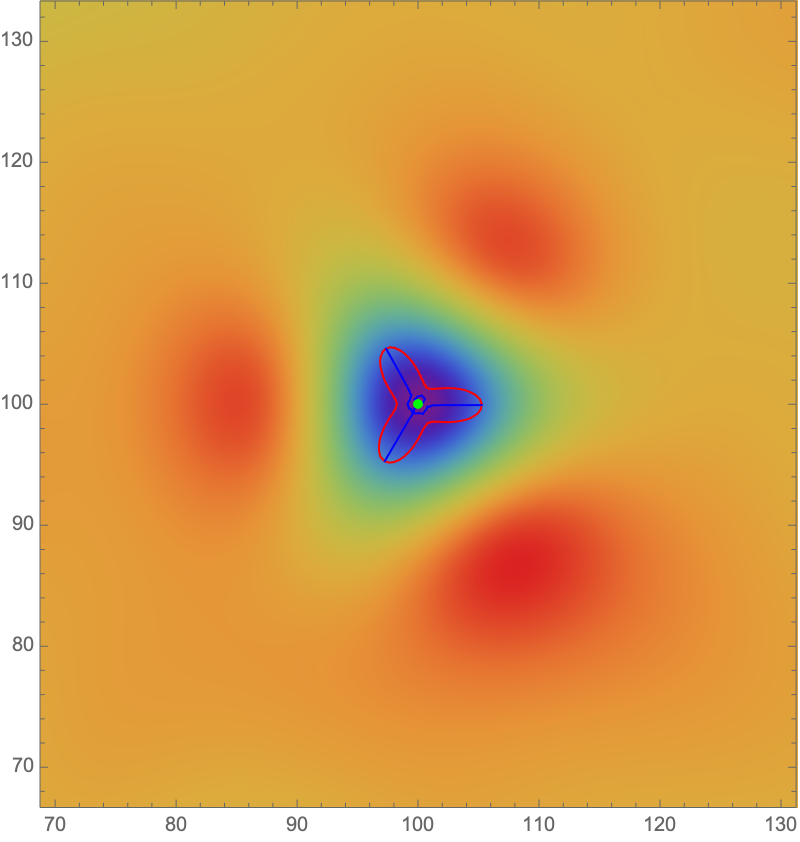
\includegraphics[width=\textwidth]{Elliptic_mean_Phi}
\end{subfigure}~
\begin{subfigure}[b]{0.32\textwidth}
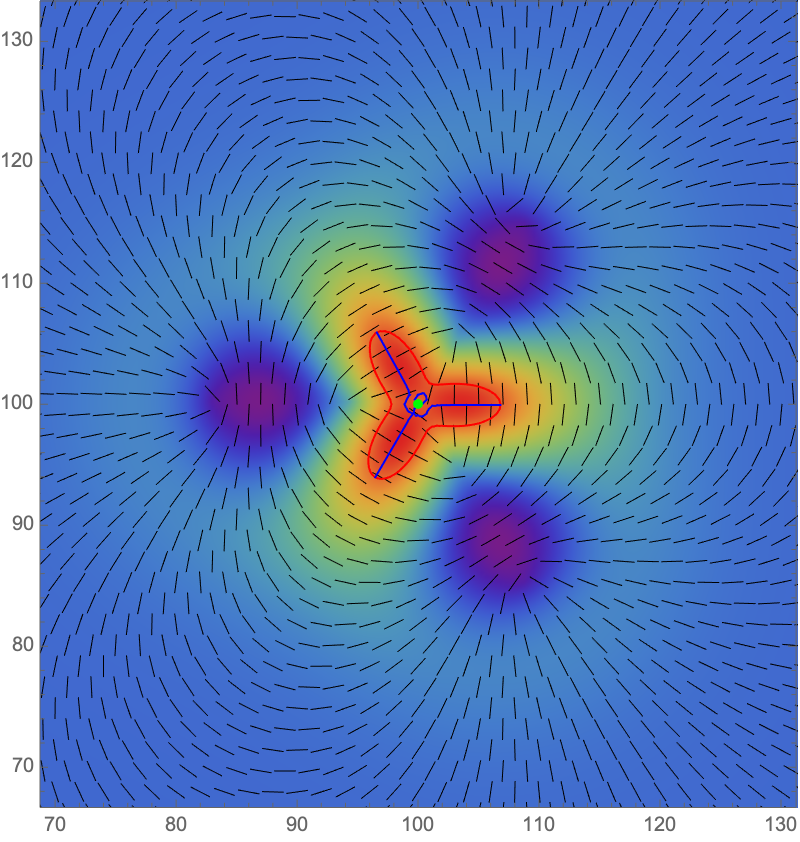
\includegraphics[width=\textwidth]{Elliptic_mean_L}
\end{subfigure}~
\begin{subfigure}[b]{0.32\textwidth}
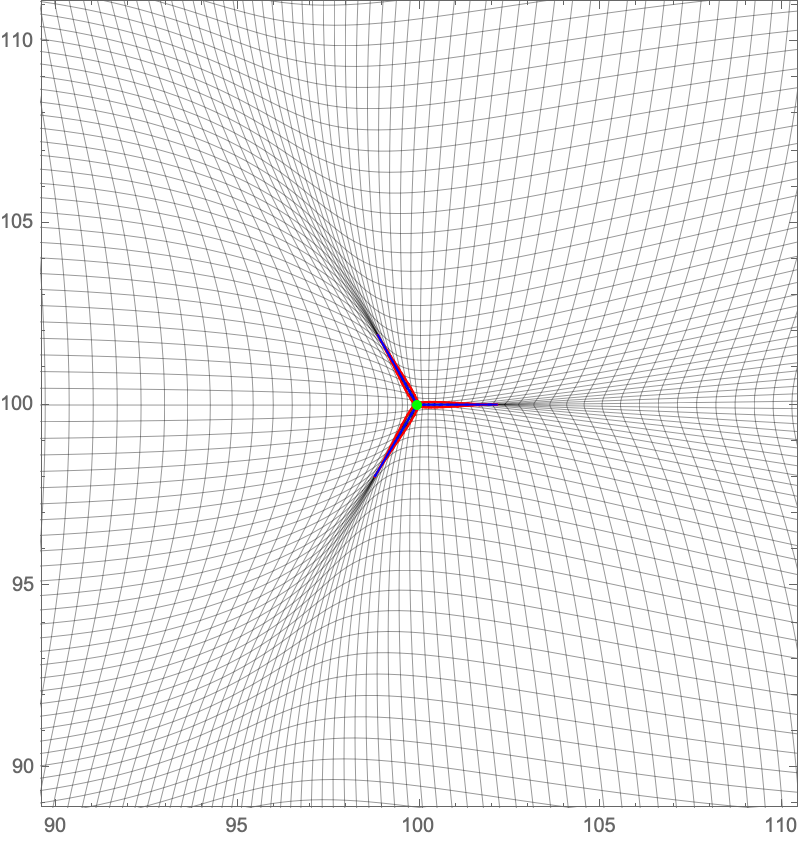
\includegraphics[width=\textwidth]{Elliptic_mean_Z}
\end{subfigure}\\
\begin{subfigure}[b]{0.32\textwidth}
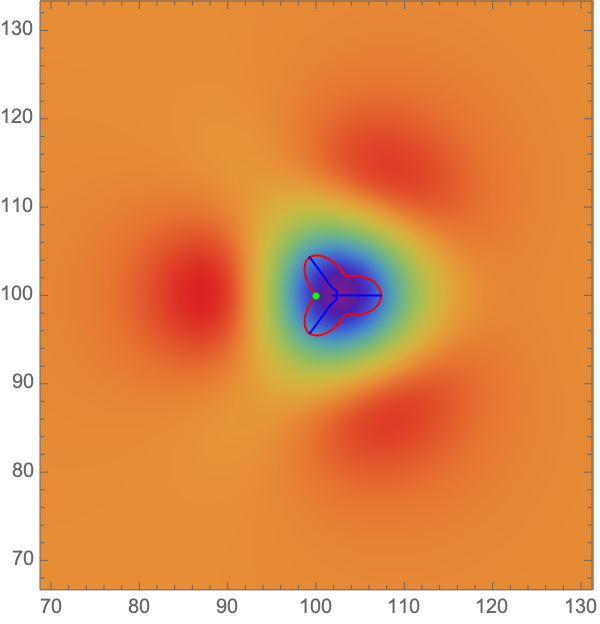
\includegraphics[width=\textwidth]{Hyperbolic_mean_Phi}
\end{subfigure}~
\begin{subfigure}[b]{0.32\textwidth}
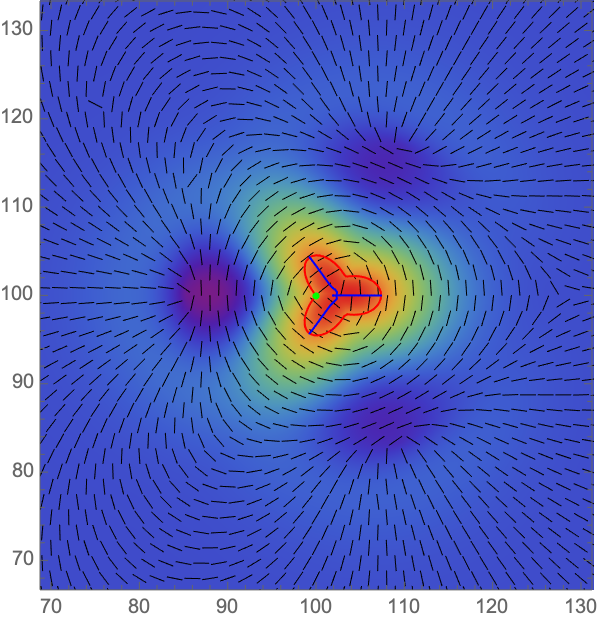
\includegraphics[width=\textwidth]{Hyperbolic_mean_L}
\end{subfigure}~
\begin{subfigure}[b]{0.32\textwidth}
\includegraphics[width=\textwidth]{Hyperbolic_mean_Z}
\end{subfigure}
\caption{The mean umbilic caustic. \textit{Upper:} the  elliptic caustic. \textit{Lower:} the hyperbolic caustic. \textit{Left:} the gravitational potential. \textit{Centre:} the first eigenvalue and eigenvector fields. \textit{Right:} The Zel'dovich approximation}\label{fig:meanHyperbolic}
\end{figure}

More generally, expand the displacement field $\bm{s}_t$ to quadratic order in $q_1$ and $q_2$ around a umbilic point at the origin $(q_1,q_2)=(0,0)$. The determinant of the gradient $\nabla \bm{x}_t$ has a critical point at the origin, as it is the product of two eigenvalue fields that vanish at the origin. The determinant takes the general form
\begin{align}
\det \nabla \bm{x}_t&=\det(I + \nabla \bm{s}_t)\nonumber\\
&= 
A q_1^2 + B q_1 q_2 + C q_2^2 + O(q_1^3,q_1^2 q_2,q_1 q_2^2,q_2^3)\,.
\end{align}
for some constants $A,B,$ and $C$.
%with
%\begin{align}
%A&= s_{1,11} s_{2,12}-s_{1,12} s_{2,11}\,,\\
%B&= s_{1,11} s_{2,22}-s_{1,22} s_{2,11}\,,\\
%C&= s_{1,12} s_{2,22}-s_{1,22} s_{2,12}\,, 
%\end{align}
%where we write the displacement field as $\bm{s}_t=(s_1,s_2)$ and the partial derivatives as $s_{i,jk}=\partial_j \partial_k s_{i}$. 
For small $q_1$ and $q_2$, the level set $\det \nabla \bm{x}_t =0$ approaches a conic section:
\begin{itemize}
\item an ellipse when the discriminant $B^2 - 4AC$ is negative corresponding to the $D_4^+$ caustic,
\item a hyperbole when the discriminant $B^2 - 4AC$ is positive corresponding to the $D_4^-$ caustic,
\item a parabola when the discriminant $B^2 - 4AC$ vanishes, corresponding to the $D_5$ caustic (which does not feature in the 2D cosmic web).
\end{itemize}
Note that the discriminant coincides with the negative of the determinant of the Hessian, \textit{i.e.},
\begin{align}
B^2-4AC = -\det \left(\mathcal{H} \left[\det \nabla \bm{x}_t \right]\right)\,.
\end{align}
When the displacement field is a gradient field, the constants $D$ and $E$ vanish and the condition reduces to the constant discussed above.

The orientation of the elliptic umbilic caustic is determined by the behavior of the eigenvector fields of the deformation tensor in the vicinity of the caustic. The fold curve in the vicinity of the elliptic umbilic caustic is a small ellipse, which forms three cusp caustics when the eigenvector field is parallel to the eigenvector field, $\bm{v}_i \cdot \bm{m} = 0$ with $\bm{m}$ the vector normal to this circle.

The orientation and configuration of the hyperbolic umbilic caustic is determined by the eigenvalues $\nu_i$ and eigenvectors $\bm{w}_i$ of the Hessian $\mathcal{H}\left[\det (I- b_+ \bm{\psi})\right]$. The cusp curve of the hyperbolic umbilic is directed towards the eigenvector corresponding to the positive eigenvalue. The angle $\beta = 2 \arctan(\sqrt{|\nu_1/\nu_2|})$ describes the angle between the two wedges of the fold curves. 


In figure \ref{fig:meanHyperbolic}, we plot the mean field of the elliptic and the swallowtail caustic. Observe that the umbilic caustics join three cusp curves and are naturally associated with the clusters of the cosmic web.

%%%%%%%%%%%%%%%%%%%%%%%%%%%%%%%%%%%%%%%%%%%%%%%%%%%%%%%%%%%%%%%%
\subsubsection{Sampling the constraint manifold}
We implement the umbilic caustics by sampling random fields with the linear constraints
\begin{align}
T_{11}&=T_{22}=1/b_+\,,\\
T_{12}&=0\,.
\end{align}
We subsequently determine the sign of the determinant $\det\left( \mathcal{H}\left[\det (I- b_+ \bm{\psi})\right]\right)$ to identify whether it is an elliptic or an hyperbolic caustic. Given the identification, we compute its orientation. By rotating the second-order and third-order derivatives (using appendix \ref{ap:rotations}), we generate linear constraint conditions corresponding to elliptic and hyperbolic caustics with a specified orientation. Given the appropriate sampling of the constraint manifold $\mathcal{M}_\mathcal{C}$, we can evaluate the mean field, the variance of the residue, and representative realizations.


%%%%%%%%%%%%%%%%%%%%%%%%%%%%%%%%%%%%%%%%%%%%%%%%%%%%%%%%%%%%%%%%
\subsection{The residue}
By definition, the residue $\delta f$ vanishes at the point where we impose the caustic condition. However, the caustic condition not only fixes the random field at a point but influences the direct environment of the condition. This behaviour is formally described by the variance in the density perturbation near the constraint (equation \eqref{eq:variance_Linear} for linear and equation \eqref{eq:variance_Nonlinear} for non-linear constraints). We can observe this behavior in the mean field and the variance of the density perturbation near the caustics (see figure \ref{fig:mean_var_dens}). Note that the statistical properties of the residue near the cusp and swallowtail caustic are not isotropic or homogeneous. However, the residue is isotropic near the umbilic caustics. For the power-law power spectrum with the Gaussian smoothing at the length scale $R_s=5\text{ Mpc}$ considered in this paper, the characteristic correlation length for the random field near the caustics is about $20\text{ Mpc}$.

\begin{figure}
\centering
\begin{subfigure}[b]{0.24\textwidth}
\includegraphics[width=\textwidth]{Cusp_mean_delta}
\end{subfigure}
\begin{subfigure}[b]{0.24\textwidth}
\includegraphics[width=\textwidth]{Swallowtail_mean_delta}
\end{subfigure}
\begin{subfigure}[b]{0.24\textwidth}
\includegraphics[width=\textwidth]{Elliptic_mean_delta}
\end{subfigure}
\begin{subfigure}[b]{0.24\textwidth}
\includegraphics[width=\textwidth]{Hyperbolic_mean_delta}
\end{subfigure}\\ \vspace{0.2\baselineskip}
\begin{subfigure}[b]{0.24\textwidth}
\includegraphics[width=\textwidth]{Cusp_mean_delta_var}
\end{subfigure}
\begin{subfigure}[b]{0.24\textwidth}
\includegraphics[width=\textwidth]{Swallowtail_mean_delta_var}
\end{subfigure}
\begin{subfigure}[b]{0.24\textwidth}
\includegraphics[width=\textwidth]{Elliptic_mean_delta_var}
\end{subfigure}
\begin{subfigure}[b]{0.24\textwidth}
\includegraphics[width=\textwidth]{Hyperbolic_mean_delta_var}
\end{subfigure}
\caption{Mean and the variance of the density field around the caustics in a $[80\text{ Mpc},120 \text{ Mpc}]^2$ box. \textit{Left to right:} the cusp, the swallowtail, the elliptic umbilic, and the hyperbolic umbilic caustic. \textit{Top:} the mean density field. \textit{Bottom:} the variance of the density field.}\label{fig:mean_var_dens}
\end{figure}

%%%%%%%%%%%%%%%%%%%%%%%%%%%%%%%%%%%%%%%%%%%%%%%%%%%%%%%%%%%%%%%%
\section{Composite constraint realizations}\label{sec:composite_constraints}
To study the interplay between the voids, walls, filaments, and clusters in the cosmic web and study the connectivity, it is important to extend the constraint theory of the caustic skeleton to include multiple constraints with specified orientations. In this section, we show how to construct realizations with composite constraints.

%%%%%%%%%%%%%%%%%%%%%%%%%%%%%%%%%%%%%%%%%%%%%%%%%%%%%%%%%%%%%%%%
\subsection{Orienting constraint conditions}\label{sec:orientation}
In section \ref{sec:caustic_skeleton_constraints}, we demonstrated a method to construct realizations of Gaussian random fields satisfying a caustic constraint at a single point with a fixed orientation. For example, we constructed realizations that included a cusp filament running vertically through the origin of the initial conditions. From the formalism, it follows that the caustic constraint can be translated to any point in the box by shifting the underlying linear functionals $\bm{C}$ (the Fourier transform of the constraints receives a phase shift). Alternatively, we can generate a realization with a cusp at the origin and translate the origin to the required location using the symmetry of the torus on which the realization lives. Unfortunately, the latter method does not work when considering multiple caustic constraints at different locations. Moreover, the second method yields difficulties for even a single caustic constraint when attempting to change the orientation with a rotation due to the symmetries of the boundary conditions of the box.

Fortunately, there exists an efficient method to generate realizations with any preferred orientation at any location:
\begin{enumerate}
\item 
Generate a realization satisfying the caustic conditions at a given point in the box with a fixed orientation as described in section \ref{sec:caustic_skeleton_constraints}. 
\item 
Analyze the derivatives in the caustic conditions. For example, from equations \eqref{eq:cusp_cond_1} and \eqref{eq:cusp_cond_2}, we note that the cusp caustic is fully determined by a number of second, third, and fourth-order derivatives.
\item
Evaluate all derivatives of the realization to the relevant order. Generally, some derivatives were obtained while sampling the constraint manifold $\mathcal{M}_\mathcal{C}$. Others do not directly influence the caustic and are sampled from the realization. For the cusp, we evaluate the partial derivatives 
\begin{align}
T_{11},T_{12},T_{22},T_{111},T_{112},T_{122},T_{222},T_{1111},T_{1112},T_{1122},T_{1222},T_{2222}\,.
\end{align}
Alternatively, we can extend the constraint manifold to include all these partial derivatives and sample them directly.
\item 
While rotating the coordinate system by an angle $\theta$, the $n$-th order derivatives transform into each other (see appendix \ref{ap:rotations}). We use these transformation rules to obtain a representative sample of the required partial derivatives for the caustic with the desired orientation.
\item 
Finally, we apply the Hoffman Ribak algorithm, with respect to the linear constraints consisting of the relevant partial derivatives, to obtain a realization satisfying the caustic condition with the desired orientation.
\end{enumerate}

See figure \ref{fig:rotation} for an illustration of the cusp caustic with three orientations. In the left panel, the cusp caustic passes vertically through the center of the box. In the central and right panels, we generate realizations for which the cusp curve passes diagonally and horizontally through the center of the box. These three realizations share a single unconstrained random field. As a consequence, we see that the structure of the initial conditions away from the center $(100,100)$ remains unchanged. Using constrained Gaussian random field theory, we can locally tweak the random field to satisfy the desired non-linear constraints.

\begin{figure}
\centering
\begin{subfigure}[b]{0.4\textwidth}
\includegraphics[width=\textwidth]{Rotation_L_1}
\end{subfigure}~
\begin{subfigure}[b]{0.4\textwidth}
\includegraphics[width=\textwidth]{Rotation_Z_1}
\end{subfigure}\\
\begin{subfigure}[b]{0.4\textwidth}
\includegraphics[width=\textwidth]{Rotation_L_2}
\end{subfigure}~
\begin{subfigure}[b]{0.4\textwidth}
\includegraphics[width=\textwidth]{Rotation_Z_2}
\end{subfigure}\\
\begin{subfigure}[b]{0.4\textwidth}
\includegraphics[width=\textwidth]{Rotation_L_3}
\end{subfigure}~
\begin{subfigure}[b]{0.4\textwidth}
\includegraphics[width=\textwidth]{Rotation_Z_3}
\end{subfigure}
\caption{The caustic skeleton consisting of the fold curves (red) and cusp curve (blue) in Lagrangian and Eulerian space with a rotation of the cusp caustic at the center of the box. \textit{Upper:} the eigenvalue and eigenvector fields in Lagrangian space. \textit{Lower:} the Zel'dovich approximation in Eulerian space. \textit{Left:} with the vertical orientation. \textit{Center:} with a diagonal orientation. \textit{Right:} with the horizontal orientation.}\label{fig:rotation}
\end{figure}


%%%%%%%%%%%%%%%%%%%%%%%%%%%%%%%%%%%%%%%%%%%%%%%%%%%%%%%%%%%%%%%%
\subsection{Multiple constraints}
In section \ref{sec:orientation}, we showed a method to orient a single non-linear constraint. In this section, we extend the treatment to multiple caustic constraints at different locations with specified orientations. 

Given the locations $\bm{q}_i$ and orientations, $\theta_i$ of the $M$ caustics constraints with $i=1,\dots,M$, one might naively repeat the analysis presented in section \ref{sec:orientation} for each constraint point and construct a realization using the Hoffman Ribak algorithm on the sampled partial derivatives. While this is a good approximation when the pairwise separation of the points $\bm{q}_i$ is larger than the typical correlation length of the random field, it fails when partial derivatives at a single point $\bm{q}_i$ become significantly correlated to the partial derivatives of a neighboring point $\bm{q}_j$. Ideally, we would sample the partial derivatives of the deformation potential at the constraint points $\bm{q}_i$ simultaneously. However, such a procedure cannot be straightforwardly implemented when sampling constraints in the eigenframe and orienting the constraints with the procedure described in the previous section.

To correct for these correlations we propose a rejection sampling method. For each caustic constraint corresponding to the point $\bm{q}_i$, we determine the $n$-th order derivatives required to specify the caustic and its orientation. Construct the conditional (unnormalized) joint probability density $p_i$ for the partial derivatives of the constraint $\bm{q}_i$ with respect to the corresponding constrained manifold $\mathcal{M}_{\mathcal{C},i}$, and the Gaussian joint probability density $p$ including all the partial derivatives at the constraint points. Next, determine the maximum $max$ of the ratio of the joint distribution of all constraints and the individual constraints $p/\prod p_i$. Finally, generate a sample of the partial derivatives satisfying the oriented caustics constraints as described above. Accept this sample with probability $p/(max\, \prod p_i)$. Alternatively, we construct the big constraint manifold $\mathcal{M}_\mathcal{C}$ by taking the union over the small constrained manifold $\mathcal{M}_{\mathcal{C},i}$, and directly sample from the conditional probability density $p(\cdot |\mathcal{M}_\mathcal{C})$ using the rejection sampling method.

\begin{figure}
\centering
\begin{subfigure}[b]{0.49\textwidth}
\includegraphics[width=\textwidth]{Composite_L}
\caption{$\lambda_1$, $\bm{v}_1$}
\end{subfigure}~
\begin{subfigure}[b]{0.49\textwidth}
\includegraphics[width=\textwidth]{Composite_Z}
\caption{Zel'dovich approximation}
\end{subfigure}
\caption{The caustic skeleton consists of the fold curves (red) and cusp curves (blue) in Lagrangian and Eulerian space, with four critical point constraints on the first eigenvalue field. \textit{Left:} the first eigenvalue and eigenvector fields in Lagrangian space. \textit{Right:} the Zel'dovich approximation in Eulerian space.}\label{fig:composite}
\end{figure}

We illustrate this procedure in figure \ref{fig:composite}, which includes four Morse point constraints on the first eigenvalue field. A critical point $\bm{q}_c$ appearing at time $t$ satisfies the condition
\begin{align}
\nabla \lambda_1(\bm{q}_c) = 0\,,\\
\lambda_1(\bm{q}_c)=1/b_+(t)\,.
\end{align}
In the eigenvector frame, this condition reduces to the linear constraints
\begin{align}
1/b_+ = T_{11} \geq T_{22}\,, \quad  T_{12}=0\,,\quad T_{111}=T_{112}=0\,.
\end{align}
See appendix \ref{ap:eigenvalueRel} for a derivation. The critical point is either a maximum, minimum -- corresponding to the Morse point $A_3^+$ -- or a saddle point -- corresponding to the Morse point $A_3^-$. We can differentiate between the two cases by evaluating the sign of the determinant of the Hessian $\mathcal{H}\lambda_1$. In the eigenframe, the Hessian takes the form
\begin{align}
\mathcal{H}\lambda_1 = 
\begin{pmatrix} 
T_{1111}+\frac{2T_{112}^2}{T_{11}-T_{22}} & T_{1112} + \frac{2 T_{112}T_{122}}{T_{11}-T_{22}} \\
T_{1112}+\frac{2 T_{112}T_{122}}{T_{11}-T_{22}} & T_{1122} + \frac{2 T_{122}^2}{T_{11}-T_{22}}
\end{pmatrix}\,.
\end{align}
See appendix \ref{ap:eigenvalueRel} for a derivation of this result. In figure \ref{fig:composite}, the lower, the lower, and the right critical points are $A_3^+$ points. The left and the upper critical points are $A_3^-$ points. In the right panel, we can clearly distinguish the character of the $A_3^+$ and $A_3^-$ points. The $A_3^+$ points correspond to the creation of a multi-stream region forming a Zel'dovich pancake. The $A_3^-$ points correspond to the merger of two multi-stream regions.



%%%%%%%%%%%%%%%%%%%%%%%%%%%%%%%%%%%%%%%%%%%%%%%%%%%%%%%%%%%%%%%%
\section{Conclusion}\label{sec:conclusion}
Developing analytic methods and systematic numerical tools for the study of the cosmic web is becoming increasingly important given the wealth of upcoming redshift surveys, as large $N$-body simulations are too expensive. In this paper, we extend constraint Gaussian random field theory to include non-linear constraints defined on a finite number of linear constraints, amounting to a subtle modification of the linear theory. Moreover, using the Hoffman-Ribak algorithm, we can efficiently sample the constraint distribution turning it into a universal tool for the study of the cosmic web (in both the two- and three-dimensional settings). The technique is applied to the two-dimensional caustic skeleton, linking the present-day voids, filaments, and clusters to non-linear conditions on the eigenvalue and eigenvector fields of the Gaussian initial gravitational potential. Applied to cosmological $N$-body simulations, the combination of non-linear constraint Gaussian random field and caustic skeleton theory pave the way towards a systematic investigation of the evolution of the progenitors of the present-day walls, filaments, and clusters, and the embedded galaxies, putting flesh on the bones of the caustic skeleton. 

The present study illustrates non-linear constraint theory with the two-dimensional caustic skeleton. However, we do not present the full implications of the framework of caustic skeleton theory. In an upcoming paper, we will analyze the properties of the constraint field in the vicinity of the different elements of the caustic skeleton in more detail. We will evaluate how the properties of the different elements of the caustic skeleton depend on the formation times. We will moreover, study how the walls, filaments, and clusters depend on their local environments in an attempt to extract the universal properties of these elements. In particular, we will analyze how the non-linear collapse of the residue with respect to the mean field influences the density profiles near the filaments and clusters of the large-scale structure. Note that, while the present analysis is restricted to the two-dimensional cosmic web, the techniques straightforwardly apply to the three-dimensional setting.

In an upcoming paper, we will:
\begin{itemize}
\item extend these studies to the three-dimensional cosmic web,
\item study the constrained initial conditions of the three-dimensional cosmic skeleton,
\item study the mean fields as a function of the formation time,
\item evaluate the eigenvalue fields and the derivatives in the eigenframes,
\item use the constrained initial conditions to study the mean density field around the different elements.
\end{itemize}

\begin{framed}
Discussion on reconstruction method. Particularly for Lagrangian fluid dynamics.
\end{framed}

\begin{framed}
  Most noteworthy is the -- as yet not yet appreciated -- the observation that filaments come in two classes \cite{Feldbrugge:2018}. The major share of the filamentary network is represented by $A_4$ swallowtail caustics, representing the sectional interfaces between two wall-like membranes. These have not yet fully collapsed along two directions. Umbilic $D_4$ caustics are also filaments, corresponding to the more prominent and dense filamentary extensions of the cluster nodes in the cosmic web and representing filaments that have fully collapsed along two directions. 
   {\color{red} This is a point of the three-dimensional cosmic web while this section is largely two-dimensional. Since we already mentioned this at another point in the introduction, I propose we move it to the discussion.}
 \end{framed}
 \cite{Cadiou:2021}
%%%%%%%%%%%%%%%%%%%%%%%%%%%%%%%%%%%%%%%%%%%%%%%%%%%%%%%%%%%%%%%%
\section*{Acknowledgement}
We thank Sergei Shandarin for having raised our interest in caustics as a key to the dynamical understanding of the cosmic web. We thank Bernard Jones for the long-standing discussions on constraint random field theory and Johan Hidding for his comments on caustic skeleton theory and its relation to constraint theory. Finally, JF would like to thank Nynke Niezink for the enlightening discussions on probability theory and statistics. JF is supported in part by the Higgs Fellowship.

%%%%%%%%%%%%%%%%%%%%%%%%%%%%%%%%%%%%%%%%%%%%%%%%%%%%%%%%%%%%%%%%

\bibliographystyle{JHEP}
% \bibliographystyle{plainnat}

\bibliography{mybibliography}

\appendix
%%%%%%%%%%%%%%%%%%%%%%%%%%%%%%%%%%%%%%%%%%%%%%%%%%%%%%%%%%%%%%%%
\section{Gaussian random fields algorithms}\label{ap:GRF}
Gaussian random fields are most naturally expressed in Fourier space, as the Fourier modes of an unconstrained Gaussian random field are normally and independently distributed, 
\begin{align}
p(\hat{f}(\bm{k}_1), \hat{f}(\bm{k}_2), \dots) = \prod_{i} \frac{1}{\sqrt{2\pi P(\bm{k}_i)}} \exp\left[-\frac{|\hat{f}(\bm{k}_i)|^2}{2P(\bm{k}_i)}\right],
\end{align}
up to the reality condition, $\hat{f}(\bm{k})=\hat{f}^*(-\bm{k})$. In this paper, we use Fast Fourier Transform routines to efficiently generate realizations of both unconstrained and linearly constrained Gaussian random.

%%%%%%%%%%%%%%%%%%%%%%%%%%%%%%%%%%%%%%%%%%%%%%%%%%%%%%%%%%%%%%%%
\subsection{Unconstrained Gaussian random fields}
We can efficiently generate realizations of unconstrained Gaussian random fields on a rectangular lattice using Fast Fourier Transform routines. The Fourier modes of an isotropic and homogeneous Gaussian random field are independent distributed Gaussian variables with zero mean, $\mu=0$, and the standard deviation $\sigma = \sqrt{P(\|\bm{k}\|)}$. Using this observation we generate the realization by multiplying the Fourier transform of white noise with the square root of the power spectrum:\\

\begin{algorithm}[H]
\SetAlgoLined
\begin{enumerate}[itemsep=1ex, leftmargin=0cm, rightmargin=1cm]
\item Generate a realization of white noise $n_w(\bm{q})$, consisting of identically independently distributed normal numbers $\mathcal{N}(\mu=0,\sigma^2=1)$ on a regular rectangular lattice.
\item Fast Fourier transform the white noise $\hat{n}_w(\bm{k}) = \text{FFT}[n_w(\bm{q})](\bm{k})$. The Fourier modes are independently normally distributed satisfying the reality condition $\hat{n}_w(\bm{k}) = \hat{n}_w^*(-\bm{k})$.
\item Rescale the Fourier modes with the power spectrum $\hat{f}(\bm{k}) = \sqrt{P(\bm{k})}\hat{n}_w(\bm{k})$.
\item Evaluate the inverse fast Fourier transform the rescaled modes to obtain the realization of the unconstrained Gaussian random field $f(\bm{q}) = \text{FFT}^{-1}[\hat{f}(\bm{k})](\bm{q})$.
\end{enumerate}
 \caption{Generating a realization of an unconstrained Gaussian random field on a rectangular lattice}
 \label{alg:GRF}
\end{algorithm}$ $\\

%%%%%%%%%%%%%%%%%%%%%%%%%%%%%%%%%%%%%%%%%%%%%%%%%%%%%%%%%%%%%%%%
\subsection{Linearly constrained Gaussian random fields}
We efficiently generate realizations of constrained Gaussian random fields, satisfying a set of linear constraints $\Gamma=\{\bm{C}[f]=\bm{c}\}$, using the Hoffman Ribak algorithm \cite{Hoffman:1991, Weygaert:1996}. The algorithm is based on the observation that the residue of the random field with respect to the mean field, $\delta f = f - \langle f | \Gamma\rangle$, is a Gaussian random field whose properties are independent of the constraint values $\bm{c}$. Note that this is a special property of Gaussianity of the random field and the linearity of the constraints $\bm{C}$.

Given an unconstrained Gaussian random field $f$ with the required power spectrum, we compute the value of the linear constraint $C_i$ using the convolution theorem
\begin{align}
C_i[f,\bm{q}_i]=\text{FFT}^{-1}[\hat{C}_i^*(\bm{k}) \hat{f}(\bm{k})](\bm{0})
\end{align}
evaluated at the origin, with the Fourier transform of the constraint $\hat{C}_i$. Assuming that the unconstrained mean field vanishes, $\langle f \rangle =0$, we evaluate the constrained mean-field using the formula
\begin{align}
\langle f(\bm{q}) | \Gamma\rangle = \sum_{i,j} \xi_i(\bm{q})\xi_{ij}^{-1} c_j\,,
\end{align}
with the covariance between the random field and the constraint
\begin{align}
\xi_i(\bm{q}) = \text{FFT}^{-1}[\hat{C}_i(\bm{k}) P(\bm{k})](\bm{q})\,,
\end{align}
and the covariance matrix of the constraints
\begin{align}
\xi_{ij}=\text{FFT}^{-1}[\hat{C}_i^*(\bm{k}) \hat{C}_i(\bm{k}) P(\bm{k})](\bm{0})\,,
\end{align}
evaluated at the origin. In these equations, we assume that $\bar{f}=\bar{C}_i=0$. Note that the vector $\bm{\xi}(\bm{q})=[\sum_i \xi_i(\bm{q}) \xi_{ij}^{-1}]$ is a normal basis of the constraints. The mean field is the inner product of $\bm{x}$ with the constraint values, 
\begin{align}
\langle f(\bm{q}) | \Gamma\rangle = \bm{\xi}(\bm{q})\cdot \bm{c}\,.
\end{align}
We use these routines to implement the Hoffman-Ribak method:\\

\begin{algorithm}[H]
\SetAlgoLined
\begin{enumerate}[itemsep=1ex, leftmargin=0cm, rightmargin=1cm]
\item Generate a realization of an unconstrained Gaussian random field $g$ with the required power spectrum using algorithm \ref{alg:GRF}.
\item Evaluate the linear constraints $C_i$ of the unconstrained field $g$,
\begin{align}
d_i = C_i[g;\bm{q}_i]\,.
\end{align} 
\item Evaluate the mean field corresponding to the constraint values $d_i$,
\begin{align}
\bar{g}(\bm{q}) = \sum_{ij}\xi_i(\bm{q}) \xi^{-1}_{ij} d_j\,.
\end{align}
\item Evaluate the residue of the unconstrained field 
\begin{align}
\delta g=g - \bar{g}\,.
\end{align}
\item Since the residue $\delta g$ is statistically independent of the values $d_j$, we can identify $\delta g$ with the residue $\delta f$ of the constrained random field. The realization of the constrained Gaussian random field takes the form
\begin{align}
f(\bm{q}) = \sum_{ij}\xi_i(\bm{q}) \xi^{-1}_{ij} c_j + \delta g(\bm{q})\,.
\end{align}
\end{enumerate}
 \caption{The Hoffman-Ribak method for Gaussian random fields with linear constraints}
 \label{alg:HoffmanRibak}
\end{algorithm}


%%%%%%%%%%%%%%%%%%%%%%%%%%%%%%%%%%%%%%%%%%%%%%%%%%%%%%%%%%%%%%%%
\section{Constraint probability density}\label{ap:constraintDensity}
The conditional density 
\begin{align}
p(f|\Gamma) =\frac{p(f, \Gamma)}{p(\Gamma)}
\end{align}
with $\Gamma = \{\bm{C} = \bm{c}\}$ is a Gaussian density as both $p(f,\Gamma)$ and $p(\Gamma)$ are normally distributed. It thus suffices to evaluate the mean and covariance matrix. For completeness, we write the mean of the function and the constraints as $\bar{f}(\bm{q})=\langle f(\bm{q}) \rangle$ and $\bar{\bm{C}}=\langle \bm{C}\rangle$, and the covariance as
\begin{align}
\xi(\bm{q}_1,\bm{q}_2)& = \text{cov}(f(\bm{q}_1),f(\bm{q}_2))= \langle (f(\bm{q}_1) - \bar{f}(\bm{q}_1))(f(\bm{q}_2) - \bar{f}(\bm{q}_2))\rangle\,,\\
\xi_i(\bm{q}) &= \text{cov}(f(\bm{q}),C_i) = \langle (f(\bm{q})-\bar{f}(\bm{q}))(C_i - \bar{C}_i)\rangle\,,\\
\xi_{ij} &= \text{cov}(C_i,C_j) = \langle (C_i - \bar{C}_i)(C_j-\bar{C}_j)\rangle\,.
\end{align}
For conciseness, we use the Einstein summation convention over the repeated dummy indices.

Define an auxiliary function $g(\bm{q}) = f(\bm{q}) + \bm{A}(\bm{q}) \cdot \bm{C}$ with $A_i(\bm{q}) = -\xi_j(\bm{q}) \xi_{ji}^{-1}$. The function $g$ is by construction independent of the variable $\bm{C}$, as they are jointly normally distributed and their covariance matrix vanishes, \textit{i.e.}, 
\begin{align}
\text{cov}(g(\bm{q}),\bm{C})
&=\text{cov}(f(\bm{q}),\bm{C}) +  \text{cov}(\bm{C},\bm{C}) \bm{A}(\bm{q})\nonumber \\
&=[\xi_k(\bm{q}) - \xi_i(\bm{q}) \xi_{ij}^{-1}\xi_{jk}]_{k=1}^N\nonumber\\
&=\bm{0}\,.
\end{align}
The expectation value of $g$ is $\langle g(\bm{q})\rangle = \bar{f}(\bm{q}) + \bm{A}(\bm{q}) \cdot \bar{\bm{C}}$, which we can use to evaluate the expectation value of the constrained field
\begin{align}
\langle f(\bm{q}) | \Gamma \rangle 
&=\langle g(\bm{q}) - \bm{A}(\bm{q})\cdot \bm{C}|\Gamma\rangle\nonumber\\
&=\langle g(\bm{q})\rangle - \bm{A}(\bm{q}) \cdot \bm{c}\nonumber\\
&=\bar{f}(\bm{q}) + \bm{A}(\bm{q})\cdot (\bar{\bm{C}}-\bm{c})\nonumber\\
&= \bar{f}(\bm{q}) + \xi_i(\bm{q})\xi_{ij}^{-1}(c_j -\bar{C}_j)\,.
\end{align}
When $\bar{f} = 0$ and $\bar{\bm{C}}=\bm{0}$ the expectation value reduces to the identity $\langle f(\bm{q}) | \Gamma \rangle =\xi_i(\bm{q})\xi_{ij}^{-1}c_j$. The covariance of the constraint field follows along similar lines
%\begin{align}
%\text{var}(f(\bm{q})|\Gamma) 
%&= \text{var}(g(\bm{q}) - \bm{A}(\bm{q})\cdot \bm{C}|\Gamma) \\
%&= \text{var}(g(\bm{q})|\Gamma) + \text{var}(\bm{A}(\bm{q})\cdot \bm{C}|\Gamma) -2 \bm{A}(\bm{q})\cdot \text{cov}(g(\bm{q}), \bm{C}|\Gamma)\\
%&= \text{var}(g(\bm{q})) \\
%&=\text{var}(f(\bm{q}) + \bm{A}(\bm{q})\cdot \bm{C})\\
%&=\text{var}(f(\bm{q})) + \bm{A}^T(\bm{q}) \text{var}(\bm{C}) \bm{A}(\bm{q}) + 2\bm{A}(\bm{q}) \cdot \text{cov}(f(\bm{q}),\bm{C}) \\
%&=\text{var}(f(\bm{q})) + \xi_i(\bm{q})\xi_{ij}^{-1}\xi_{jk}\xi_{kl}^{-1}\xi_{l}(\bm{q}) - 2\xi_i(\bm{q})\xi_{ij}^{-1}\xi_{j}(\bm{q})\\
%&=\xi(\bm{0}) - \xi_i(\bm{q}) \xi_{ij}^{-1} \xi_j(\bm{q})\,.
%\end{align}
\begin{align}
\text{cov}(f(\bm{q}_1), f(\bm{q}_2)|\Gamma) 
&= \text{cov}(g(\bm{q}_1) - \bm{A}(\bm{q}_1)\cdot \bm{C}, g(\bm{q}_2) - \bm{A}(\bm{q}_2)\cdot \bm{C}|\Gamma) \nonumber\\
&= \text{cov}(g(\bm{q}_1), g(\bm{q}_2)|\Gamma) + \text{cov}(\bm{A}(\bm{q}_1)\cdot \bm{C}, \bm{A}(\bm{q}_2)\cdot \bm{C}|\Gamma)\nonumber\\
&\ \ \  - \bm{A}(\bm{q}_1)\cdot \text{cov}(\bm{C}, g(\bm{q}_2)|\Gamma) -\text{cov}(g(\bm{q}_1) , \bm{C}|\Gamma)\cdot \bm{A}(\bm{q}_2)\nonumber\\
&= \text{cov}(g(\bm{q}_1), g(\bm{q}_2)) \nonumber\\
&=\text{cov}(f(\bm{q}_1) + \bm{A}(\bm{q}_1)\cdot \bm{C}, f(\bm{q}_2) + \bm{A}(\bm{q}_2)\cdot \bm{C})\nonumber\\
&=\text{cov}(f(\bm{q}_1), f(\bm{q}_2)) + \bm{A}(\bm{q}_1) \text{cov}(\bm{C},\bm{C}) \bm{A}^T(\bm{q}_2) \nonumber\\
&\ \ \ + \bm{A}(\bm{q}_1) \cdot \text{cov}(\bm{C},f(\bm{q}_2))+ \text{cov}(f(\bm{q}_1), \bm{C}) \cdot \bm{A}(\bm{q}_2) \nonumber\\
&=\text{cov}(f(\bm{q}_1), f(\bm{q}_2)) + \xi_i(\bm{q}_1)\xi_{ij}^{-1}\xi_{jk}\xi_{kl}^{-1}\xi_{l}(\bm{q}_2) - 2\xi_i(\bm{q}_1)\xi_{ij}^{-1}\xi_{j}(\bm{q}_2)\nonumber\\
&=\xi(\bm{q}_1,\bm{q}_2) - \xi_i(\bm{q}_1) \xi_{ij}^{-1} \xi_j(\bm{q}_2)\,.
\end{align}
We conclude that the residue $\delta f$ of $f$ with respect to the mean field $\langle f(\bm{q})|\Gamma\rangle =\bar{f}(\bm{q})+ \xi_i(\bm{q})\xi_{ij}^{-1}(c_j-\bar{C}_j)$ is a Gaussian random field with zero mean $\langle \delta f|\Gamma\rangle=0$ and variance $\langle \delta f(\bm{q})^2|\Gamma\rangle = \sigma_0^2 - \xi_i(\bm{q}) \xi_{ij}^{-1} \xi_j(\bm{q})$. Note that the residue $\delta f$ for a Gaussian random field with linear constraints is indeed independent of $\bm{c}$. The covariance of the constraint field yields the constrained probability density
\begin{align}
p(f|\Gamma) \propto  \exp\left[-\frac{1}{2} \iint \delta{f}(\bm{q}_1) \tilde{K}(\bm{q}_1,\bm{q}_2) \delta f(\bm{q}_2)\mathrm{d}\bm{q}_1 \mathrm{d}\bm{q}_2 \right]
\end{align}
with the residue $\delta f = f-\bar{f}(\bm{q})+ \xi_i(\bm{q})\xi_{ij}^{-1}(c_j-\bar{C}_j)$ and the kernel $\tilde{K}$ defined as the inverse of the modified two-point correlation function, \textit{i.e.},
\begin{align}
\int \tilde{K}(\bm{q}_1,\bm{q}) \left[\xi(\bm{q},\bm{q}_2) - \xi_i(\bm{q})\xi_{ij}^{-1}\xi_j(\bm{q}_2)\right]\mathrm{d}\bm{q}= \delta_D^{(2)}(\bm{q}_1-\bm{q}_2)\,.
\end{align}
The correction $- \xi_i(\bm{q})\xi_{ij}^{-1}\xi_j(\bm{q}_2)$ implements the statistical anisotropy and inhomogeneity of the residue.


%%%%%%%%%%%%%%%%%%%%%%%%%%%%%%%%%%%%%%%%%%%%%%%%%%%%%%%%%%%%%%%%
\section{Non-linear eigenvalue relations: a direct approach}\label{ap:eigenvalueRel}
The eigenvalue and eigenvector fields are non-linear functions of the deformation tensor
\begin{align}
\bm{\psi} = \begin{pmatrix} T_{11} & T_{12} \\ T_{12} & T_{22}\end{pmatrix},
\end{align}
with the partial derivatives of the displacement potential $T_{ijk\dots} = \frac{\partial}{\partial q_i}\frac{\partial}{\partial q_j}\frac{\partial}{\partial q_k}\dots \Psi$. In two dimensions, the eigenvalue and eigenvector fields are the quadratic roots of the eigenequation $\bm{\psi}\bm{v}_i=\lambda_i \bm{v}_i$, with the explicit identities for the eigenvalue fields
\begin{align}
\lambda_1(T_{11},T_{22},T_{12}) &= \frac{1}{2}\left(T_{11}+T_{22} + \sqrt{4 T_{12}^2 +(T_{11}-T_{22})^2}\right)\,,\label{eq:lambda_1}\\
\lambda_2(T_{11},T_{22},T_{12}) &= \frac{1}{2}\left(T_{11}+T_{22} - \sqrt{4 T_{12}^2 +(T_{11}-T_{22})^2}\right)\,.\label{eq:lambda_2}
\end{align}
The study of Gaussian random fields satisfying non-linear caustic constraints is most concisely performed in the eigenframe, for which $T_{12}=0$ and $T_{11} \geq T_{22}$ leading to the eigenvalues $\lambda_1=T_{11}, \lambda_2=T_{22}$ and and eigenvectors
\begin{align}
\lambda_{1} &= T_{11}\,,\quad \bm{v}_1=(1,0)\,,\\
\lambda_{2} &= T_{22}\,,\quad \bm{v}_2=(0,1)\,.
\end{align}
In this section, we give an explicit derivation of several identities relating to the partial derivatives of the eigenvalue and eigenvector fields and the partial derivatives of the displacement potential in the eigenframe, using an Euler angle. In appendix \ref{ap:eigenvalueRel_alt}, we present a more efficient algebraic derivation, which more easily generalizes to the three-dimensional setting.

Using an eigenvalue decomposition we can write the deformation tensor as $\bm{\psi} = R^T \Lambda R,$ with the diagonal matrix
\begin{align}
\Lambda = \begin{pmatrix}\lambda_1 & 0 \\ 0 &\lambda_2 \end{pmatrix}
\end{align}
with the ordering $\lambda_1 \geq \lambda_2$, and the rotation matrix
\begin{align}
R = \begin{pmatrix} \cos \theta & - \sin \theta \\ \sin \theta & \cos \theta \end{pmatrix} \in SO(2),
\end{align}
with the Euler angle $\theta$. The decomposition yields three identities for the components of the deformation tensor $T_{11},T_{22},T_{12}$ 
\begin{align}
T_{11} &= \lambda_1 \cos^2 \theta + \lambda_2 \sin^2 \theta\,,\\
T_{22} &= \lambda_1 \sin^2\theta + \lambda_2 \cos^2 \theta\,,\\
T_{12} &= (\lambda_2 - \lambda_1)\cos \theta \sin \theta\,.
\end{align}
Solving for the Euler angle $\theta$, we obtain a representation for the normalized eigenvector fields
\begin{align}
\bm{v}_1 &=\pm (\cos(\theta), -\sin(\theta))\,,\\
\bm{v}_2 &=\pm (\sin(\theta),\ \ \ \cos(\theta))\,,
\end{align}
where the sine and cosine are expressed in terms of the partial derivatives of the displacement potential
\begin{align}
\cos(\theta) &= \frac{\sqrt{T_{11} - T_{22} + \sqrt{4 T_{12}^2 +(T_{11}-T_{22})^2}}}{\sqrt{2} \sqrt[4]{4T_{12}^2 + (T_{11}-T_{22})^2}}\,,\\
\sin(\theta) &= \frac{\sqrt{2}T_{12}}{\sqrt[4]{4T_{12}^2+(T_{11}-T_{22})^2}\sqrt{T_{11}-T_{22} + \sqrt{4T_{12}^2 + (T_{11}-T_{22})^2}}}\,.
\end{align}
These relations enable us to evaluate several useful non-linear identities. We evaluate the derivatives of the eigenvalue field in a general frame and subsequently take the limit $T_{12} \to 0$ with the condition $T_{11}\geq T_{22}$. 

The first-order derivatives of the eigenvalue fields in the eigenframe satisfy the linear equations
\begin{align}
\nabla \lambda_1&= (T_{111}, T_{112})\,,\\
\nabla \lambda_2&= (T_{122}, T_{222})\,.
\end{align}
The second order derivatives receive a non-linear correction
\begin{align}
\frac{\partial^2}{\partial q_1^2} \lambda_1&= T_{1111} + \frac{2 T_{112}^2}{T_{11}-T_{22}}\,,\\
\frac{\partial^2}{\partial q_1 \partial q_2} \lambda_1&= T_{1112} + \frac{2 T_{112}T_{122}}{T_{11}-T_{22}}\,,\\
\frac{\partial^2}{\partial q_2^2} \lambda_1&= T_{1122} + \frac{2T_{122}^2}{T_{11}-T_{22}}\,,\\
\frac{\partial^2}{\partial q_1^2} \lambda_2&= T_{1122} - \frac{2 T_{112}^2}{T_{11}-T_{22}}\,,\\
\frac{\partial^2}{\partial q_1 \partial q_2} \lambda_2&= T_{1222} - \frac{2 T_{112}T_{122}}{T_{11}-T_{22}}\,,\\
\frac{\partial^2}{\partial q_2^2} \lambda_2&= T_{2222} - \frac{2T_{122}^2}{T_{11}-T_{22}}\,.
\end{align}

The first-order derivative in the direction of the eigenvalue field naturally coincides with the first-order derivatives described above
\begin{align}
\bm{v}_1 \cdot \nabla \lambda_1 &= \pm T_{111}\,,\quad
\bm{v}_2 \cdot \nabla \lambda_1 = \pm T_{112}\,,\\
\bm{v}_1 \cdot \nabla \lambda_2 &= \pm T_{122}\,,\quad
\bm{v}_2 \cdot \nabla \lambda_2 = \pm T_{222}\,.
\end{align}
Note that these combinations transform as scalars under rotations. The second-order derivatives receive an additional non-linear term due to the variation of the eigenvector fields. The second-order derivatives of the first eigenvalue field take the form
\begin{align}
\bm{v}_1 \cdot \nabla (\bm{v}_1 \cdot \nabla \lambda_1) &= T_{1111} + \frac{3T_{112}^2}{T_{11}-T_{22}}\,,\\
\bm{v}_2 \cdot \nabla (\bm{v}_1 \cdot \nabla \lambda_1) &= \pm \left[T_{1112} + \frac{3T_{112}T_{122}}{T_{11}-T_{22}}\right]\,,\\
\bm{v}_1 \cdot \nabla (\bm{v}_2 \cdot \nabla \lambda_1) &= \pm \left[T_{1112} - \frac{T_{112}(T_{111}-2T_{122})}{T_{11}-T_{22}}\right]\,,\\
\bm{v}_2 \cdot \nabla (\bm{v}_2 \cdot \nabla \lambda_1) &= T_{1122} - \frac{T_{122}(T_{111}-2T_{122})}{T_{11}-T_{22}}\,.
\end{align}
Note that the directional derivatives in the directions $\bm{v}_1$ and $\bm{v}_2$ do not commute. The second-order derivatives of the second eigenvalue field yield the analogous identities
\begin{align}
\bm{v}_1 \cdot \nabla (\bm{v}_1 \cdot \nabla \lambda_2) &= T_{1122} + \frac{T_{112}(T_{222}-2T_{112})}{T_{11}-T_{22}}\,,\\
\bm{v}_2 \cdot \nabla (\bm{v}_1 \cdot \nabla \lambda_2) &= \pm\left[T_{1222} + \frac{T_{122}(T_{222}-2T_{112})}{T_{11}-T_{22}}\right]\,,\\
\bm{v}_1 \cdot \nabla (\bm{v}_2 \cdot \nabla \lambda_2) &= \pm\left[T_{1222} - \frac{3T_{112}T_{122}}{T_{11}-T_{22}}\right]\,,\\
\bm{v}_2 \cdot \nabla (\bm{v}_2 \cdot \nabla \lambda_2) &= T_{2222} - \frac{3T_{122}^2}{T_{11}-T_{22}}\,.
\end{align}

%%%%%%%%%%%%%%%%%%%%%%%%%%%%%%%%%%%%%%%%%%%%%%%%%%%%%%%%%%%%%%%%
\section{Non-linear eigenvalue relations: an algebraic approach}\label{ap:eigenvalueRel_alt}
Unfortunately, the derivation of the non-linear eigenvalue relations presented in appendix \ref{ap:eigenvalueRel} does in practice not straightforwardly generalize to the three-dimensional case. It formally works but is not sufficiently efficient in practice. However, using an algebraic approach we can reproduce the results presented in section \ref{ap:eigenvalueRel} more efficiently. This method does generalize to the higher-dimensional setting. We present this derivation here for the two-dimensional case in anticipation of an upcoming paper on the three-dimensional caustic skeleton and constraint random fields \cite{Feldbrugge:2022}.

In two dimensions, the eigenvalue fields are related to the principle invariants of the deformation tensor
\begin{align}
\text{Tr}\ \bm{\psi} &= T_{11} + T_{22} = \lambda_1 + \lambda_2\,,\label{eq:principle_1}\\
\text{det}\ \bm{\psi} &=  T_{11}  T_{22} - T_{12}^2 = \lambda_1 \lambda_2\,.\label{eq:principle_2}
\end{align}
Assuming $T_{11} > T_{22}$ and the ordering $\lambda_1> \lambda_2$ these equations have a unique solution (see equations \eqref{eq:lambda_1} and \eqref{eq:lambda_2}). In the eigenframe, $T_{12}=0$, we will assume the orientations $\bm{v}_1=(1,0)$ and $\bm{v}_2=(0,1)$. 

Now, apply the differential operators $\partial_i$ and $\partial_{i}\partial_j$ for $i,j=1,2$ to equations \eqref{eq:principle_1} and \eqref{eq:principle_2} to obtain a set of five equations. Rotate to the eigenframe by substituting $\lambda_1 = T_{11}$, $\lambda_2=T_{22}$, and $T_{12}=0$ and solve for $\partial_i\lambda_j$ and $\partial_i \partial_j \lambda_k$. The equations have a unique solution that coincides with the partial derivatives of the eigenvalue fields presented in appendix \ref{ap:eigenvalueRel}.

To evaluate the directional derivatives of the eigenvalue fields in the direction of the eigenvectors, we use the chain rule 
\begin{align}
\bm{v}_i \cdot \nabla (\bm{v}_j \cdot \nabla \lambda_k)= (\bm{v}_i \cdot  \nabla )\bm{v}_j \cdot \nabla \lambda_k + \bm{v}_i (\mathcal{H} \lambda_k )\bm{v}_j \,,
\end{align}
with the Hessian $\mathcal{H}$. We already obtained identities for the derivatives of the eigenvalue fields in the eigenframe. What remains is the evaluation of the derivative of the eigenvector fields $(\bm{v}_i \cdot \nabla) \bm{v}_j$. First note that the normalization $\|\bm{v}_i\|=1$ implies the identity
\begin{align}
\bm{v}_i \cdot \partial_j \bm{v}_i=0\,.\label{eq:normal_v}
\end{align} 
The vector $\partial_i \bm{v}_j$ is normal to $\bm{v}_j$. In addition, application of the operator $\partial_j$ on the eigenequation $(\bm{\psi}-\lambda_i I)\bm{v}_i=\bm{0}$ yields the identity
\begin{align}
(\partial_j \bm{\psi} - \partial_j \lambda_i I)\bm{v}_i + (\bm{\psi}-\lambda_i I)\partial_j \bm{v}_i=\bm{0}\,. \label{eq:eigen_d}
\end{align}
Note that this equation does not yield a unique solution since the matrix $\bm{\psi}-\lambda_i I$ is singular. However, the combined system of equation \eqref{eq:normal_v} with \eqref{eq:eigen_d} is solvable. In the eigenframe, we obtain the gradient of the eigenvector fields
\begin{align}
\nabla \bm{v}_1 &= \begin{pmatrix}
0, & T_{112}/(T_{11}-T_{22})\\
0, & T_{122}/(T_{11}-T_{22})
\end{pmatrix},\\
\nabla \bm{v}_2 &= \begin{pmatrix}
-T_{112}/(T_{11}-T_{22}), & 0\\
-T_{122}/(T_{11}-T_{22}), & 0
\end{pmatrix}.
\end{align}
When combining the derivatives of the eigenvalue and eigenvector fields, we reproduce the remaining results presented in appendix \ref{ap:eigenvalueRel}.

%%%%%%%%%%%%%%%%%%%%%%%%%%%%%%%%%%%%%%%%%%%%%%%%%%%%%%%%%%%%%%%%
\section{Rotations of derivatives of the deformation tensor}\label{ap:rotations}
Under a rotation, the derivatives of the deformation tensor transform nontrivially. When applying the rotation matrix
\begin{align}
R_\theta = \begin{pmatrix} c  & s  \\- s  & c \end{pmatrix},
\end{align}
with $c=\cos\theta$ and $s=\sin \theta$, the first, second, third, and fourth-order derivatives transform into each other. The first-order derivatives transform as a vector
\begin{align}
\begin{pmatrix} T_1 \\ T_2 \end{pmatrix}
\mapsto
\begin{pmatrix}
c & -s \\
s &  c 
\end{pmatrix}
\begin{pmatrix} T_1 \\ T_2 \end{pmatrix}.
\end{align}
The second-order derivatives transform as
\begin{align}
\begin{pmatrix} T_{11} \\ T_{12} \\ T_{22} \end{pmatrix}
\mapsto
\begin{pmatrix}
c^2 & -2 c s    &  s^2 \\
c s &  c^2- s^2 & -c s \\
s^2 & 2c s      &  c^2 
\end{pmatrix}
\begin{pmatrix} T_{11} \\ T_{12} \\ T_{22} \end{pmatrix}.
\end{align}
The third-order derivatives transform as
\begin{align}
\begin{pmatrix} T_{111} \\ T_{112} \\ T_{122}\\ T_{222} \end{pmatrix}
\mapsto
\begin{pmatrix}
c^3   & -3 c^2 s        & 3 c s^2          & -s^3   \\
c^2 s &  c(c^2 - 2 s^2) & s( s^2- 2 c^2)   &  c s^2 \\
c s^2 &  s(2 c^2 - s^2) & c(c^2 -  2 s^2)  & -c^2 s \\
s^3   &  3 c s^2        & 3 c^2 s          & c^3 
\end{pmatrix}
\begin{pmatrix} T_{111} \\ T_{112} \\ T_{122}\\ T_{222} \end{pmatrix}.
\end{align}
The fourth-order derivatives transform as
\begin{align}
\begin{pmatrix} T_{1111} \\ T_{1112} \\ T_{1122}\\ T_{1222} \\ T_{2222} \end{pmatrix}
\mapsto
\begin{pmatrix}
c^4     & -4 c^3 s          & 6 c^2 s^2               &- 4 c s^3          &  s^4     \\
c^3 s   & c^2(c^2 - 3 s^2)  & 3cs(s^2 - c^2)     & s^2(3 c^2  - s^2) & -c s^3   \\
c^2 s^2 & 2cs( c^2 -  s^2)  & c^4  - 4 c^2 s^2  + s^4 & 2cs(  s^2 -  c^2) &  c^2 s^2 \\
c s^3   & s^2(3 c^2  - s^2) & 3cs( c^2 - s^2 )   & c^2(c^2  - 3 s^2) & -c^3 s   \\
s^4     & 4cs^3             & 6 c^2 s^2               & 4 c^3 s           &  c^4 
\end{pmatrix}
\begin{pmatrix} T_{1111} \\ T_{1112} \\ T_{1122}\\ T_{1222} \\ T_{2222} \end{pmatrix}.
\end{align}
\end{document}
